\documentclass[12pt]{report}
\usepackage{auphd}     % For Ph.D.
\usepackage{ulem}       % underlining on style-page; see \normalem below
\usepackage{url}
\usepackage{tikz}
\usepackage{pgf}
\usepackage{inconsolata}
\usepackage{caption,subcaption}
\usepackage[hidelinks]{hyperref}
\usepackage{listings}
\usepackage{amsmath}
\usepackage{float}
\lstset{tabsize=2,basicstyle=\footnotesize\ttfamily}


%%%%%Format rules: Normal margins are 1 in. If you need to print with 1.5in margins, uncomment the line below
%\oddsidemargin0.5in \textwidth6in

%% If you do not need a List of Abbreviations, then comment out the lines below and the \printnomenclature line.
%%for List of Abbreviations information:  (see http://www.mackichan.com/TECHTALK/509.htm  )
\usepackage[intoc]{nomencl}
\renewcommand{\nomname}{List of Abbreviations}   	       
\makenomenclature
%% don't forget to run:   makeindex ausample.nlo -s nomencl.ist -o ausample.nls

% May want theorems numbered by chapter
\newtheorem{theorem}{Theorem}[chapter]

% Put the title, author, and date in. 
\title{Improving Vehicular Networking Reliability and Efficiency in Context of Platooning Applications}
\author{Song Gao} 
\date{May, 2016} %date of graduation
\copyrightyear{2016} %copyright year

\keywords{Dedicated Short Range Communication, Wireless Access in Vehicular Environment, Computer Networks, Vehicular Networking, Wireless Networking, Vehicle Platooning, Emulation, IEEE 802.11, Compression, Bandwidth, Congestion, Reliability}

% Put the Thesis Adviser here. 
\adviser{Alvin Lim}


% Put the committee here (including the adviser), one \professor for each. 
% The advisor must be first, and the dean of the graduate school must be last.
\professor{Alvin Lim, Chair, Professor of Computer Science and Software Engineering}
\professor{Saad Biaz, Professor of Computer Science and Software Engineering}
\professor{Hari Narayanan, John H. and Gail Watson Professor of Computer Science and Software Engineering}
\professor{Xiao Qin, Professor of Computer Science and Software Engineering}

\begin{document}

\begin{romanpages}      % roman-numbered pages 

\TitlePage

\chapter*{Acknowledgements}
\addcontentsline{toc}{chapter}{Acknowledgements}%

TODO

\begin{abstract} 
  Vehicular networking is a technology that enables vehicles communication system. A joint effort from the automobile industry, transportation industry, and government offices is driving the adoption of this technology to build intelligent transportation systems that consist of smart vehicles. This study attempts to improve the reliability and efficiency of vehicular networking. The study assumes the context of platooning applications, but the contributions of this study can be applied to other vehicular applications as well.

  There are two contributions in this study. First, a wireless emulator is designed and implemented to emulate IEEE 802.11 networks in real-time using the Ethernet infrastructure. The emulator replaces the MAC layer and physical layer of IEEE 802.11 networking stack with a real-time CSMA/CA model, thus reduces the cost of experiments. It provides upper layers the same interfaces as on a real device. As a result, the testing targets in the emulation are real-world software components as opposed to simulation scripts in a discrete event simulator. These software components can be routing protocols, transport protocols, or applications, and are the same code that can be deployed in real-world.

  Second, an Interframe Compression Transmission Layer is designed and implemented, to provide efficient transmission of periodical messages in vehicular environments. The transmission layer compresses the difference between frames instead of frames themselves, and reduces bandwidth consumption significantly. To improve the behaviors of the transmission layer under different scenarios and configurations studied, an adaptive version of the algorithm is designed, which achieves more than 50\% in reduction of bandwidth consumption using real-world platooning data trace. With lower bandwidth consumption, delivery ratio is vastly improved in congested networking environments.
\end{abstract}

\tableofcontents
\listoffigures
\listoftables

\printnomenclature[1.0in] %used for the List of Abbreviations
\end{romanpages}        % All done with roman-numbered pages


\normalem       % Make italics the default for \em

\chapter{Introduction and Motivation}
Dedicated Short Range Communication (DSRC\nomenclature{DSRC}{Dedicated Short Range Communication}), is a communication technology designed for vehicular environments. By utilizing wireless radio, DSRC allows vehicles to communicate with nearby vehicles and road-side units efficiently. Wireless device vendors have been actively developing chipsets and integrated modules that provides DSRC support. Integrated devices that provides not only DSRC, but also supports for GPS and Controller Area Network (CAN\nomenclature{CAN}{Control Area Network}) bus are also in market \cite{aradasystems,denso,unex}. Automobile and transportation companies have also been actively integrating DSRC into vehicles and developing various DSRC-enabled applications.

Thanks to its low latency advantage, DSRC enables various applications that, among many other benefits, can enhance safety by augmenting human drivers' operations. Many of such applications have been designed or prototyped. An intersection collision warning system, for example, can emit warning messages through DSRC when a vehicle is going too fast towards an intersection with a red traffic light, so that other vehicles and pedestrians can be notified to avoid collision. As another example, an emergency braking warning system enables the vehicle to ``see" another vehicle in front braking hard when the line-of-sight is blocked by a large vehicle, so that the vehicle can promptly decelerate before the driver realizes the situation.

Among many safety related DSRC applications, vehicle platooning, or cooperative adaptive cruise control \cite{fhwa2015report}, provides many incentives to commercial companies. It frees drivers from throttling and braking control by delegating it to the vehicle's computer and communication system. In addition to the safety enhancement, platooning makes vehicles run closer to each other. This improves aerodynamic efficiency and results in lower fuel cost. This study starts from this use case, and tries to improve efficiency and reliability of vehicular networking.

DSRC is a recent technology that was just standardized a few years ago. It has not been deployed to vehicles in the market yet. Most studies have focused on interactions with a few vehicles only. However, when the majority of vehicles on roads are equipped with DSRC, the wireless channels will be heavily utilized, and there can be scalability problems. This study looks at these potential problems, and tries to provide a way to improve efficiency and reliability of DSRC networking services.

There are two major contribution in this study:
\begin{itemize}
  \item First, a wireless emulator is designed and implemented to emulate DSRC networks. It provides a way to test DSRC applications in a scalable way, using real application software. Unlike simulation approach where simulation scripts need to be written in order to test the idea, in the emulator the testing targets are application softwares that can be directly deployed in real-world devices.
  \item Second, a compression technique, Interframe Compression Transmission Layer (ICTL\nomenclature{ICTL}{Interframe Compression Transmission Layer}), is proposed. The compression layer compresses the difference between consecutive frames, rather than the frames themselves. It reduces bandwidth consumption in vehicular applications, particularly those that periodically sends messages that do not change dramatically. By reducing the bandwidth consumption, it makes channel congestions less likely to happen. Behaviors of ICTL under different configuration and scenarios are studied, and the findings lead to the design of an adaptive ICTL algorithm, which further lowers bandwidth consumption compared to the basic ICTL algorithms.
\end{itemize}

\chapter{Background}

\section{Dedicated Short Range Communication}

\begin{figure}[htb]
  \begin{center}
    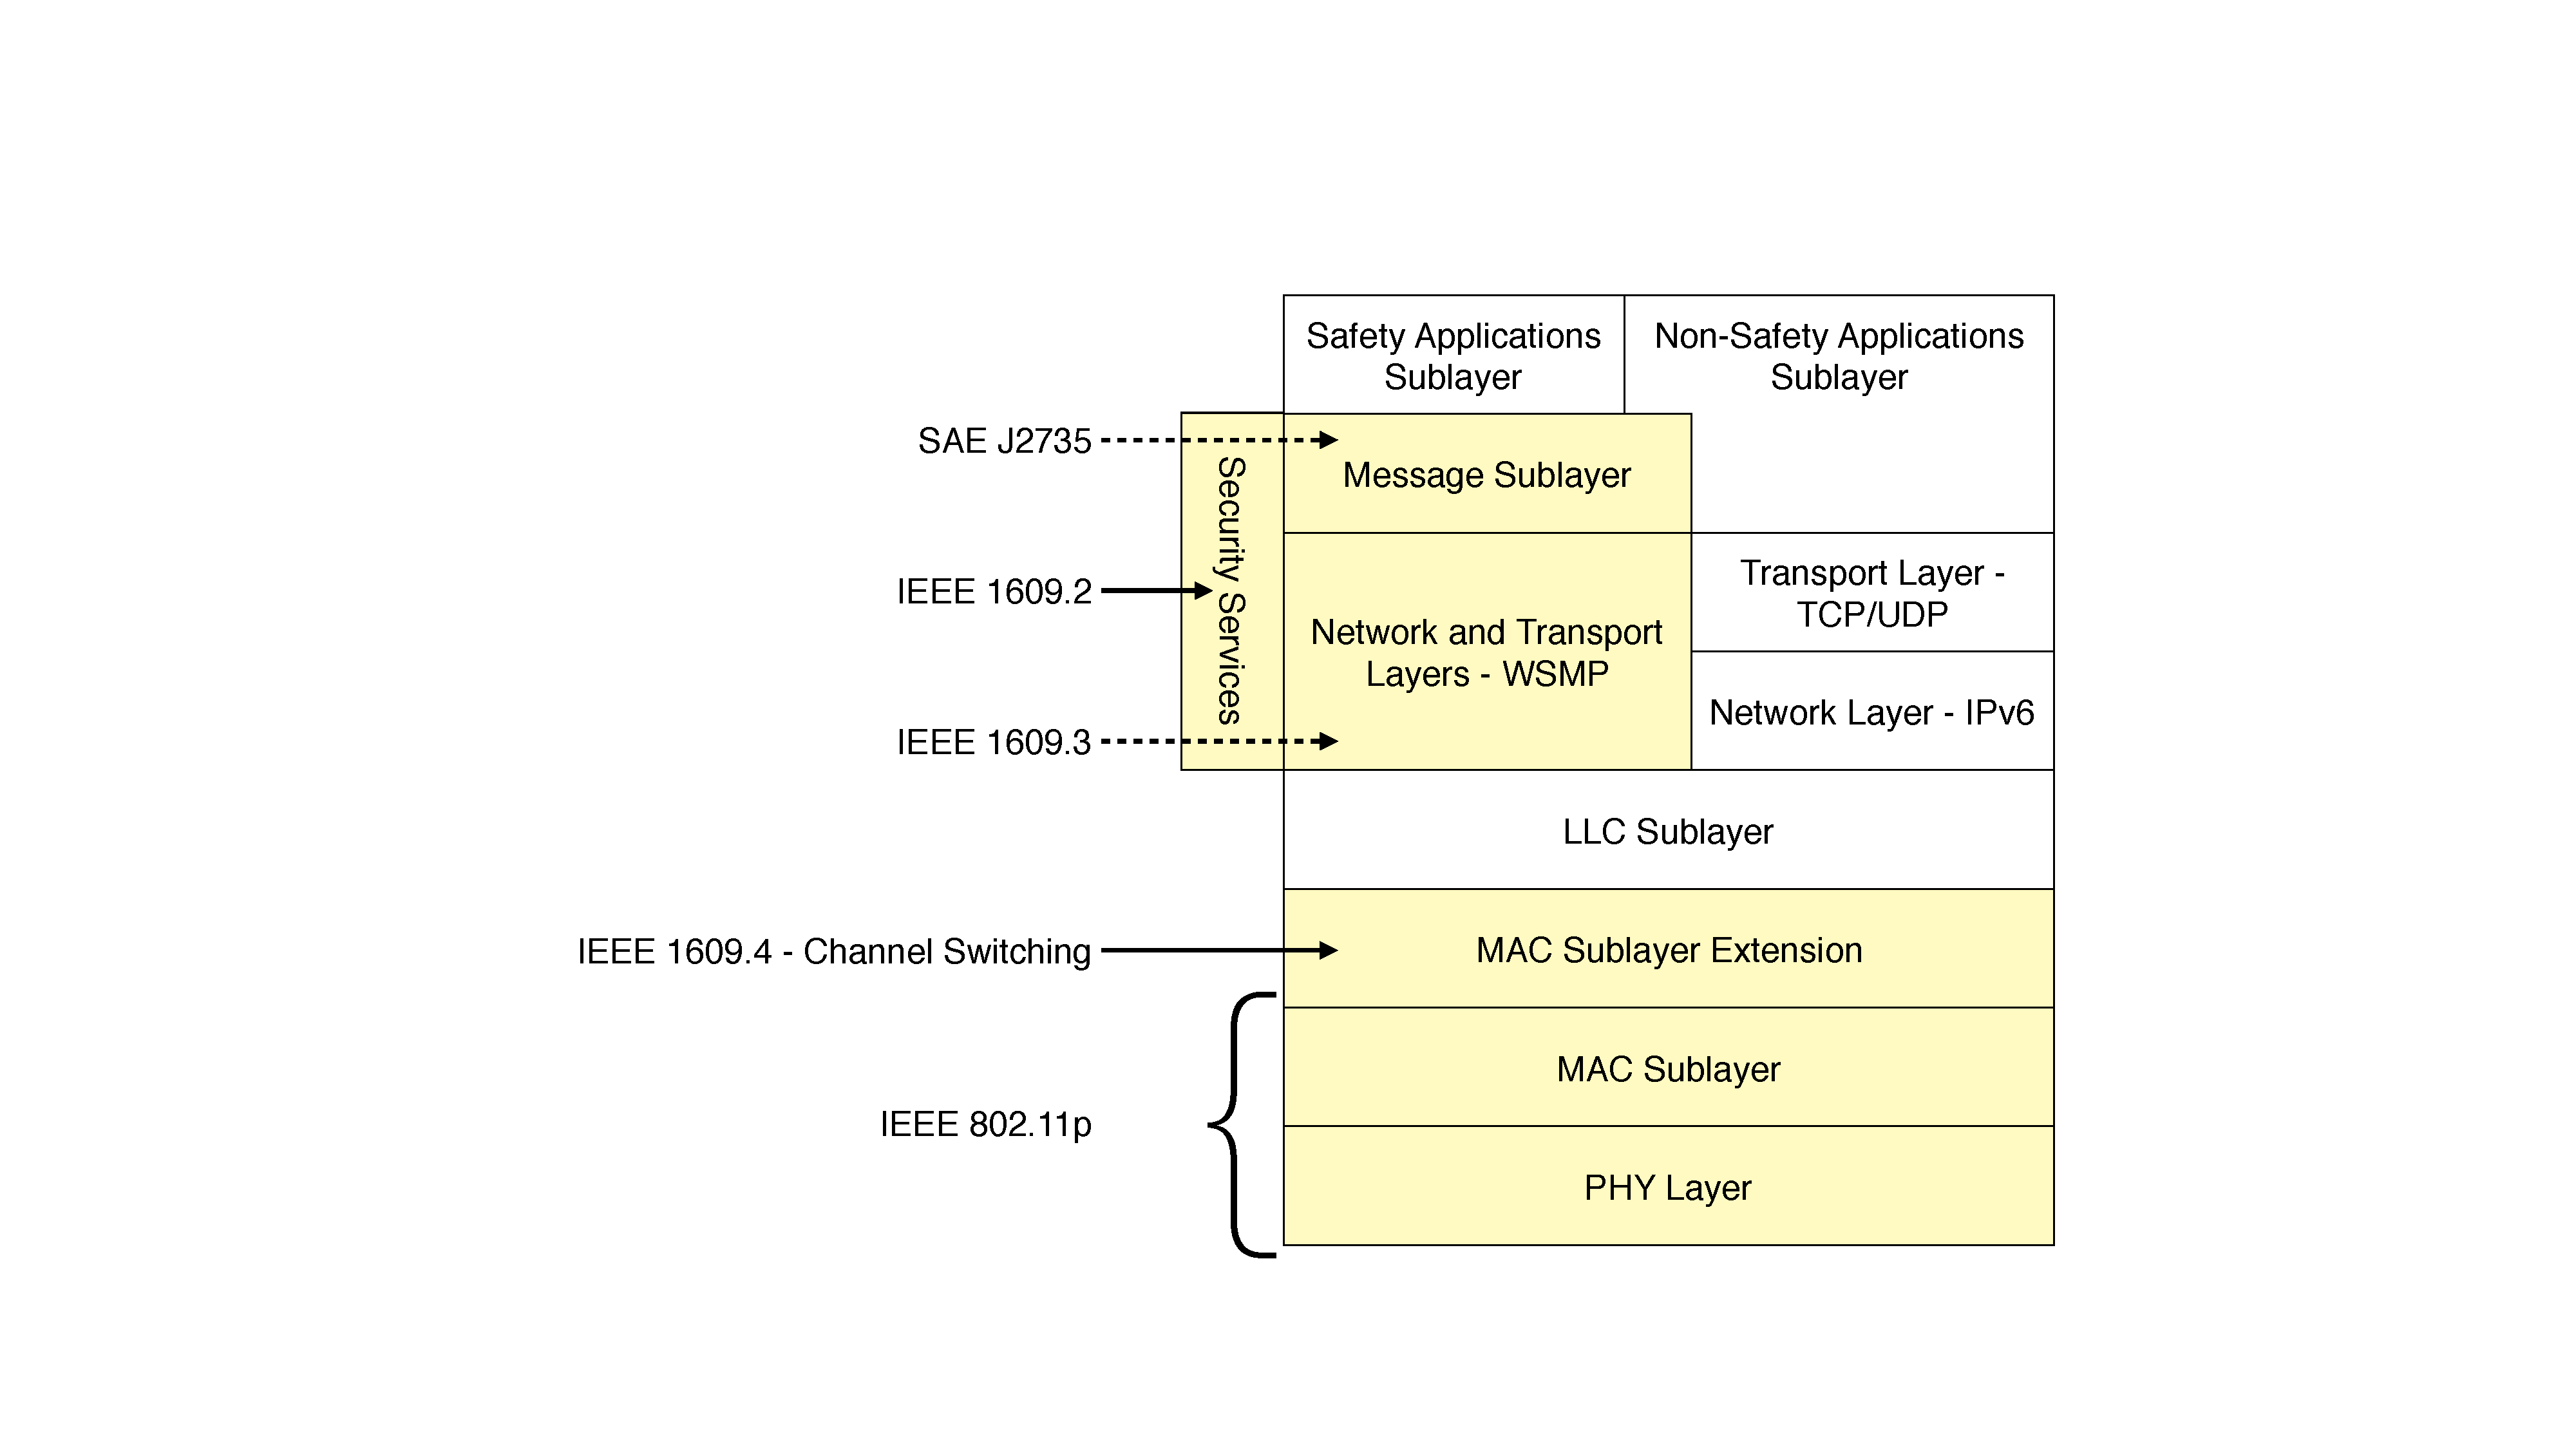
\includegraphics[width=.7\columnwidth]{figures/dsrc.pdf}
    \caption{\label{fig:dsrc}DSRC protocol suite.}
  \end{center}
\end{figure}

DSRC, also known as Wireless Access in Vehicular Environment (WAVE\nomenclature{WAVE}{Wireless Access in Vehicular Environment}), is a protocol suite designed for low latency networking in vehicular environments. The protocol suite \cite{kenney2011}, as illustrated in Figure~\ref{fig:dsrc}, is similar to TCP/IP over WiFi. In fact, it supports the IPv6 stack in parallel with a network and transport layer protocol called Wave Short Message Protocol (WSMP\nomenclature{WSMP}{Wave Short Message Protocol}) that is dedicated to the DSRC suite. Since the WSMP stack is required to be used in safety applications such as platooning, this study focuses on the WSMP branch of the protocol suite.

\subsection{IEEE 802.11p}
\label{sec:80211p}
IEEE 802.11p is derived from IEEE 802.11a, an early 5 GHz protocol used in WiFi. The Federal Communications Commission (FCC\nomenclature{FCC}{Federal Communications Commission}) has allocated the spectrum from 5.850 GHz to 5.925 GHz, i.e., the ``5.9 GHz band", for DSRC operation in United States \cite{fcc59allocation}. This spectrum is divided into seven 10 MHz channels (channel 172, 174, 176, 178, 180, 182, 184) with 5 MHz guard band at the low end \cite{kenney2011}. Chanel $<174, 176>$ and $<180, 182>$ can be combined into 20 MHz channels. This spectrum is higher than the unlicensed 5.8 GHz spectrum used in the WiFi protocols, so DSRC applications do not suffer from interference generated by WiFi devices. As in the IEEE 802.11a protocol, the IEEE 802.11p uses Orthogonal Frequency Division Multiplexing (OFDM\nomenclature{OFDM}{Orthogonal Frequency Division Multiplexing}) for modulation and Carrier Sense Multiple Access/Collision Avoidance (CSMA/CA\nomenclature{CSMA/CA}{Carrier Sense Multiple Access/Collision Avoidance}) for medium access control.

Table~\ref{tab:data_rate} shows data rates \cite{kenney2011} for different modulation types and coding rates. With the same modulation type and same coding rate, 10 MHz channel gets only half the data rate compared to 20 MHz channels. As a result, the available bandwidth in upper layer is reduced by half as well.

\begin{table}[htb]
  \begin{center}
    \begin{tabular}{|c|c|c|c|}
      \hline
      Modulation & Coding & Data rate & Data rate     \\
      Type       & Rate   & 20 MHz    & 10 MHz        \\\hline
      BPSK       & 1/2    & 6         & 3             \\\hline
      BPSK       & 3/4    & 9         & 4.5           \\\hline
      QPSK       & 1/2    & 12        & 6             \\\hline
      QPSK       & 3/4    & 18        & 9             \\\hline
      16-QAM     & 1/2    & 24        & 12            \\\hline
      16-QAM     & 3/4    & 36        & 18            \\\hline
      64-QAM     & 2/3    & 48        & 24            \\\hline
      64-QAM     & 3/4    & 54        & 27            \\\hline
    \end{tabular}
    \caption{\label{tab:data_rate}Data Rate in Mbps for 10 MHz and 20 MHz channels}
  \end{center}
\end{table}

Unlike other IEEE 802.11 protocols where stations have to join a Basic Service Set (BSS\nomenclature{BSS}{Basic Servie Set}) before they can transmit or receive data, IEEE 802.11p defines an Outside Context of BSS (OCB\nomenclature{OCB}{Outside Context of BSS}) mode for the WSMP branch of the protocol suite. In OCB mode, Basic Service Set Identification (BSSID\nomenclature{BSSID}{Basic Service Set Identification}) field of the frame header is set to a wildcard value \texttt{FF:FF:FF:FF:FF:FF}. It allows stations to transmit and receive data without registering with an infrastructure device or an existing Ad-hoc network. As a result, the time required to activate a wireless device is significantly reduced.

In addition, the Media Access Control (MAC\nomenclature{MAC}{Media Access Control}) sub-layer has an extension that supports channel switching, defined in IEEE 1609.4 \cite{ieee16094}. One of the seven 10 MHz channels is dedicated as the control channel (CCH\nomenclature{CCH}{Control Channel}) while others work as service channels (SCHs\nomenclature{SCH}{Service Channel}). Channel switching allows concurrent access of CCH and SCHs. This is achieved by dividing each 100 milliseconds into a 46 milliseconds CCH interval and a 46 milliseconds SCH interval, each followed by a 4 milliseconds guard interval. Inherently, channel switching reduces usable bandwidth of the CCH to about half of that without channel switching.

\subsection{Wave Short Message Protocol}
WSMP, defined in IEEE 1609.3 \cite{ieee16093}, is the networking service in DSRC and serves the purposes of the network layer and transport layer from the TCP/IP stack. WSMP defines a message type that is efficient for 1-hop transmission. The message type is called Wave Short Message (WSM\nomenclature{WSM}{Wave Short Message}), whose minimum header size is 5 bytes, as shown in Table~\ref{tab:wsm}. Compared to UDP over IPv6, which is a similar configuration in the TCP/IP protocol stack that requires a minimum of 52 bytes of header, WSM's overhead is much smaller and causes less congestion. Since channel congestion is a significant concern in DSRC, the efficiency of WSMP is quite valuable \cite{kenney2011}. On the other hand, being such a minimum protocol, WSMP does not provide many powerful transport layer functionalities other than multiplexing, which is achieved through the Provider Service Identifier (PSID\nomenclature{PSID}{Provider Service Identifier}) field in the WSM header.

\begin{table}[h]
  \begin{center}
    \begin{tabular}{|c|c|c|c|c|c|}
      \hline
      Version & PSID      & Extension   & Element ID & Length  & Payload \\ \hline
      1 byte  & 1-4 bytes & variable    & 1 byte     & 2 bytes & variable \\ \hline
    \end{tabular}
    \caption{\label{tab:wsm}WSM Header}
  \end{center}
\end{table}

\subsection{Message Sub-layer}
On top of the WSMP layer is the Message Sub-layer, which directly provides support to applications. An important standard in this layer is the SAE J2735 DSRC Message Set \cite{sae2016j2735}. J2735 defines many message types that vehicular applications can utilize. The messages are encoded using ASN.1 format and always transmitted with WSMP. Each message is defined as a collection of constituent data structures called data elements and data frames. A data element is the most basic data structure in the J2735 standard. A data frame has a more complex data structure, and is composed of one or more data elements or other data frames. \cite{kenney2011} These data structures carry various information related to vehicular environment, from geometries of vehicle body to the dynamics of a running vehicle.

\section{Vehicle Platooning}
Vehicle platooning is one of safety applications that DSRC enables. In vehicle platooning, Cooperative Adaptive Cruise Control (CACC\nomenclature{CACC}{Cooperative Adaptive Cruise Control}) plays an important role. CACC is based on Adaptive Cruise Control (ACC\nomenclature{ACC}{Adaptive Cruise Control}, also known as Autonomous/Active Cruise Control), which in addition to maintaining speed as in normal Cruise Control, can adjust vehicle speed based on distance between the vehicle and other vehicles in front of it, i.e., headway distances. The distance detection relies on radar sensors mounted at the front of the vehicle. Due to the latency from the time when a front vehicle brakes to the time when the ACC enabled vehicle reacts to the decreased headway, safe following distance is set to be quite high in ACC systems. In CACC, however, headway distance can be further decreased without introducing extra safety issues. As shown in Figure~\ref{fig:brake}, this is achieved by a signaling mechanism that results in shorter reaction time when then front vehicle is braking. In this mechanism, as soon as the front vehicle's driver hit the brake pedal, even before the front vehicle starts to decelerate, the braking signal, along with other information, is broadcast through DSRC, making the vehicle that is following closely aware of the situation and brake in advance. Since this mechanism does not completely rely on actual headway distance change and sensor accuracy, the headway distance can be further reduced, to a point where the aerodynamic context can change significantly.

\begin{figure}[htb]
  \begin{center}
    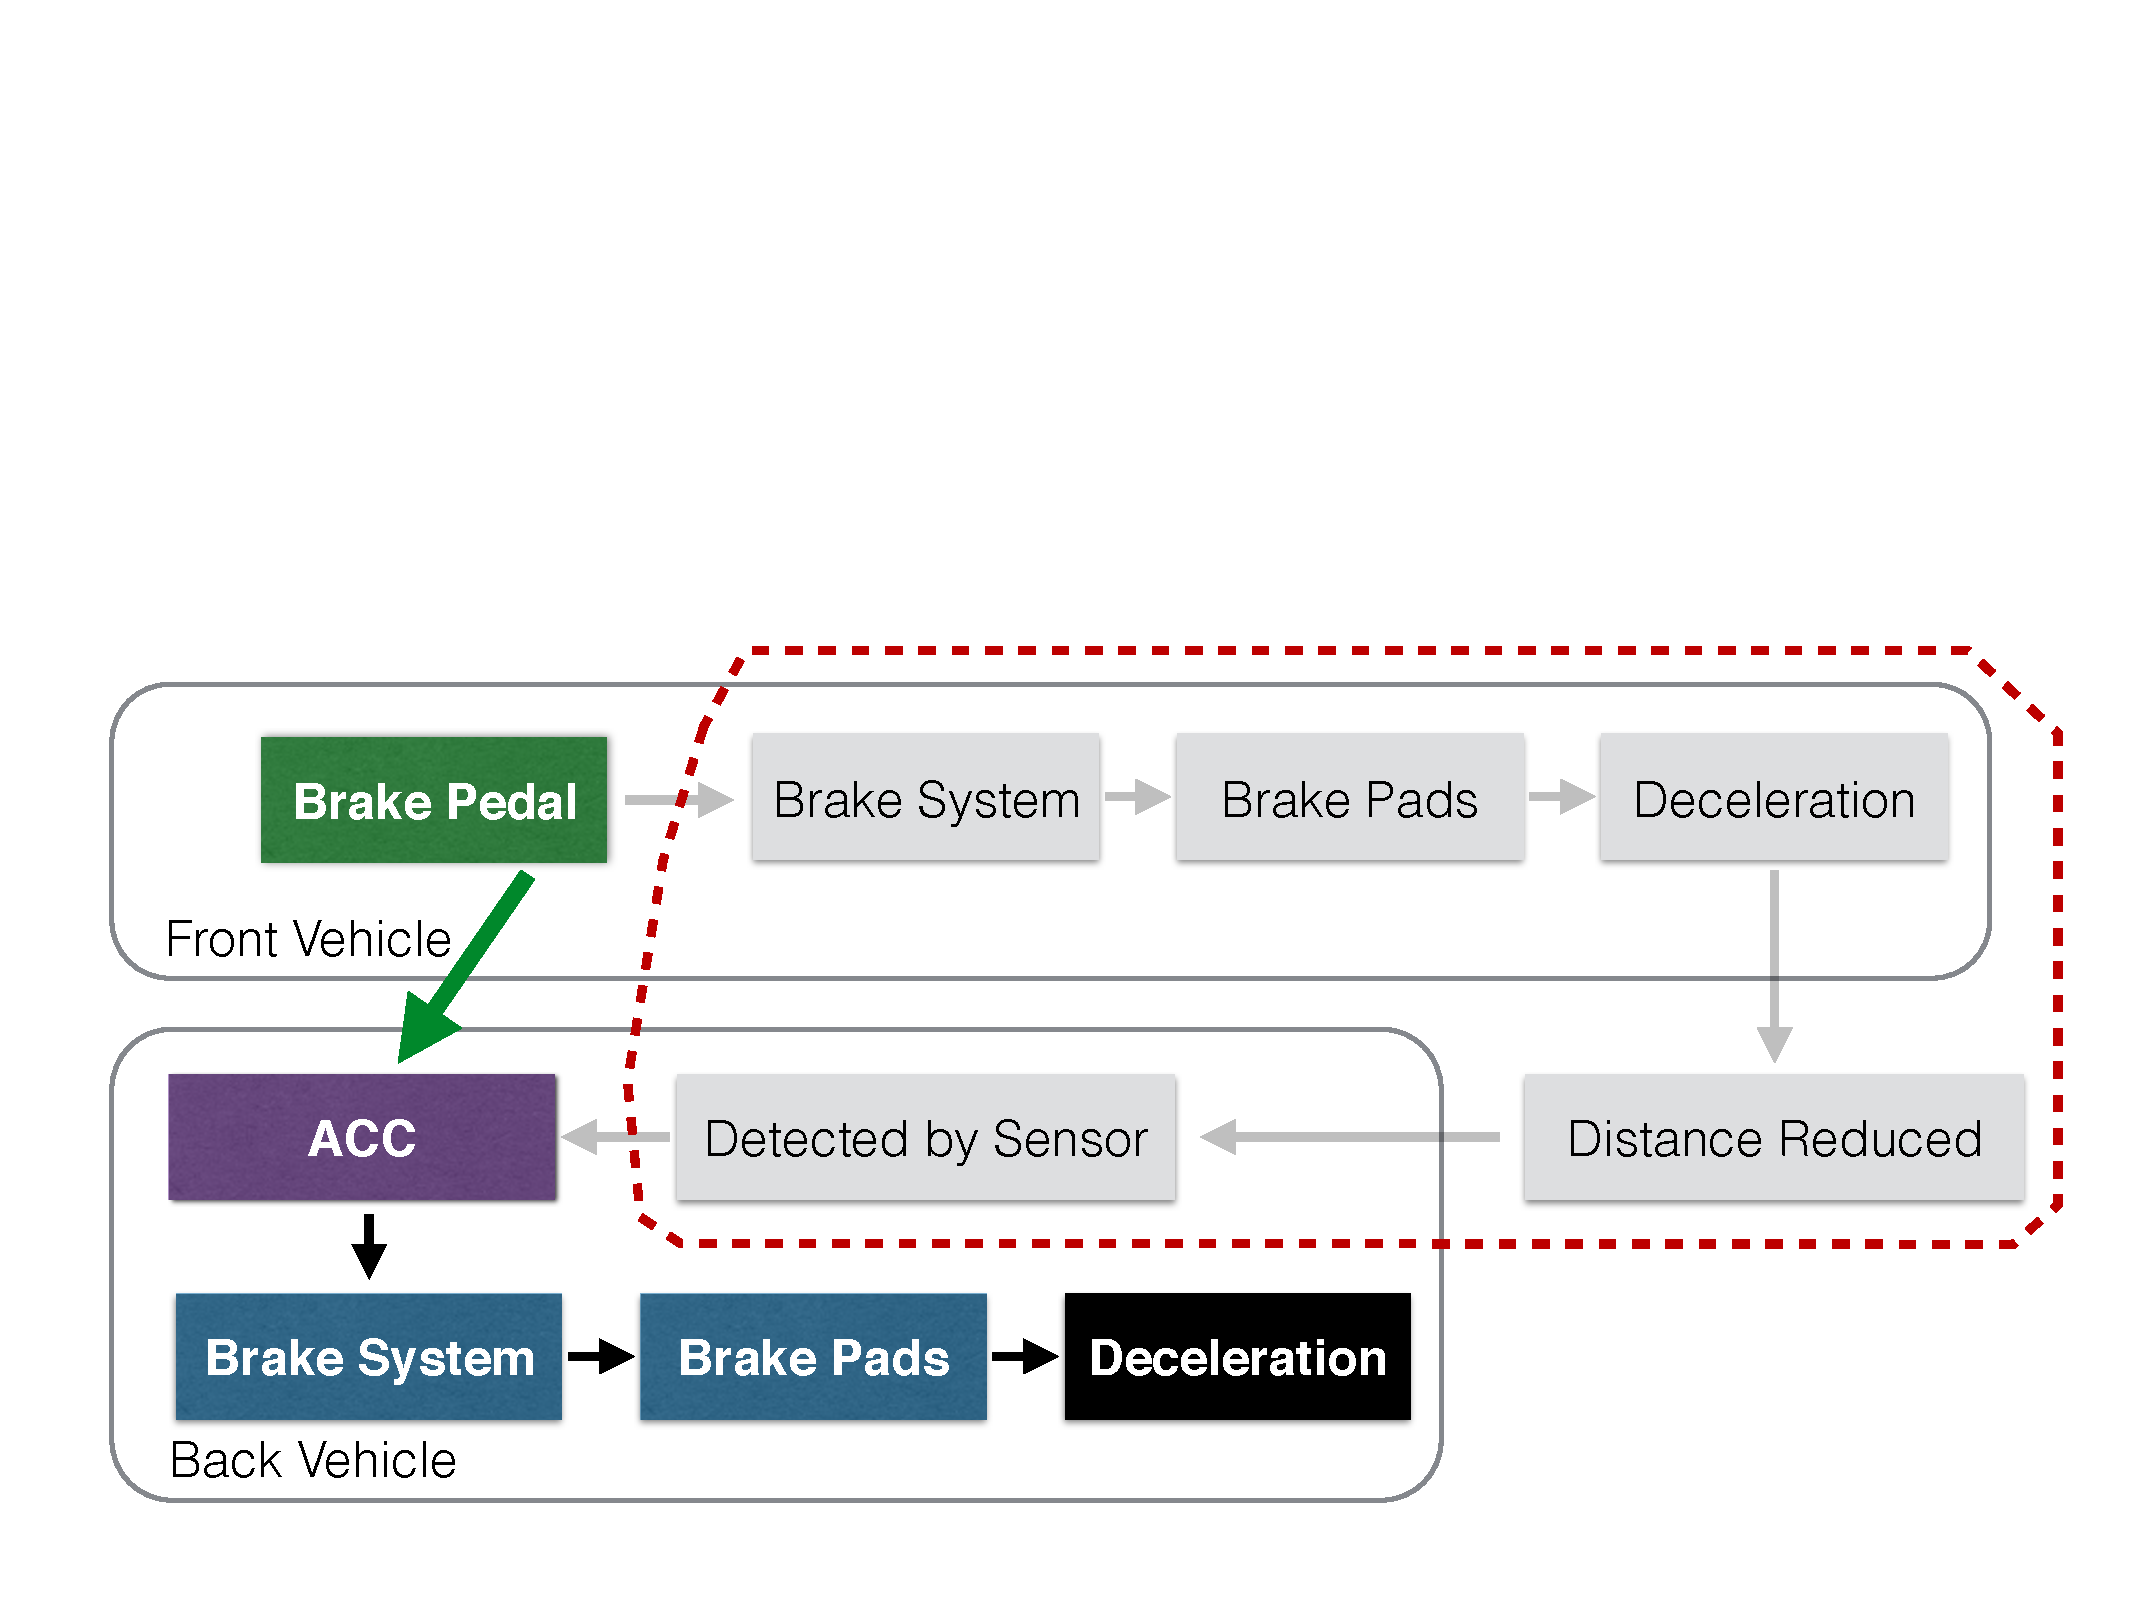
\includegraphics[width=.7\columnwidth]{figures/brake.pdf}
    \caption{\label{fig:brake}CACC shortcuts control flow of ACC thus reduces reaction time.}
  \end{center}
\end{figure}

Close following distance might not be very appealing to consumer cars, but it brings huge benefits to big commercial vehicles. To be specific, short following distance can reduce air resistance (drag) for the vehicles \cite{watts2015computational,fhwa2015report}, and the drag reduction results in fuel saving (up to 11\% in some scenarios \cite{lammert2014effect}). This is of great interest to transportation companies. For example, in trucking industry, the single largest operating cost is diesel fuel, being 34\% in year 2014 in the US \cite{atri2015analysis}. 11\% fuel saving yields 3.74\% saving of the total operating cost.

\section{Real-world Performance Attributes of DSRC in Platooning Scenarios}

\label{sec:background_realworld_performance}

In a real-world deployment, antenna's mounting position matters because vehicle body can block line-of-sight and affects wireless propagation. The vehicle body can block the line-of-sight between the vehicle's antenna and vehicles next to it. The problem becomes greater for large size vehicles, such as semi-trailer trucks. To solve this problem, many researchers and engineers choose to mount two DSRC antennas on the vehicle \cite{Bergenhem20121222,peloton}. Many DSRC device vendors provide devices with two antenna interfaces \cite{aradasystems,denso,unex}.

A straightforward and easy-to-implement way to make the communication more reliably with dual-antenna design is to replicate each message on both antennas. In other words, the DSRC stack is configured to use both antennas alternately and each message is sent twice through DSRC. This way, as long as one side of antennas makes it through, the message can be delivered. It improves reliability but uses twice as much bandwidth, causing more channel congestion.

To obtain better understanding on how well DSRC can support platooning applications, we conducted an experimental study in which we conducted extensive real-world DSRC tests using two semi-trailer trucks\cite{songDSRC2016}, primarily focusing on delivery ratio of broadcast messages under various circumstances and with different parameters. Tests conducted in this study included a set of dynamic tests with two trucks running on a 1.7-mile test track as a general case and a few sets of static tests for studying performance in specific scenarios, such as when the road was not horizontal or when the front vehicle was turning.

In the study we used three antenna operating mode: alternate, left, and right. For alternate mode, we introduced pairwise delivery ratio. It is similar to the normal delivery ratio, except that it represents the ratio of the messages delivered from either of a pair of antennas to the total pairs of messages sent. In pairwise delivery ratio, delivery of any one of a pair of duplicate messages indicates successful transmission of the pair. 

The study concluded that many factors can result in reduction in delivery ratio for broadcast messages. For example,

\begin{itemize}
  \item if the front vehicle is turning, outside antenna is blocked by the vehicle body and results in poor delivery ratio;
  \item on straight road, some terrain can affect delivery ratio significantly;
  \item on hilly road, vehicle needs to rely on terrain's reflection because antennas are not parallel.
\end{itemize}

However, in all scenarios, using alternate mode improves delivery ratio significantly. To be more specific, the pairwise delivery ratio is above $90\%$ for data rates up to 6 Mbps in all scenarios, even when using a side antenna only delivers less than $20\%$ messages. In some scenarios, alternate mode even achieves above $90\%$ delivery ratio for 27 Mbps. \cite{songDSRC2016} For the dissertation, this is an important conclusion from the study. It suggests that it is most feasible to use alternate mode all the time. Since alternate mode requires more bandwidth, how to reduce bandwidth while maintaining reliability becomes a more important issue to solve.

\chapter{Emulation Infrastructure}

\section{Problem Statement}
\label{sec:problem_validation}

In networking, there are three experimental approaches to validate an algorithm or a protocol: real-world experiments, simulations, and emulations.

In real-world experiments, real wireless devices, such as DSRC radios, or laptops with WiFi cards, are used. An operating system with complete networking stack is installed on such devices, and applications can use various APIs to access the wireless hardware for real wireless communication. The algorithm being validated runs on top of existing protocols, or replaces an existing software component running on the device. Real-world experiments provide the most realistic results, since they are real experiments using hardware and software components that are used in the real-world. The disadvantage of real-world experiments is that they are hard to conduct and require expensive devices and human resources to scale.

In simulation approach, everything is replaced by software components. A common way to implement network simulation is to use a discrete event simulator. The simulator converts the complex system into an ordered sequence of well defined events. The more specific the events are, the more accurate the simulation results will be and the more time it will take to run the simulation. It is normally easier to scale to large number of nodes with simulation, but since all hardware and software components are simulated, the accuracy of the simulation results largely relies on the quality of simulation models of each layer being simulated. In addition, once an idea is validated in simulation, it needs to be re-implemented as real software components in order to be used in real-world. Any bug in simulation scripts or the real implementation can result in different behaviors between the two. Thus, results from simulations become less trustworthy.

Emulations are a balance between real-world experiments and simulation approach. In emulations, some parts of the system are replaced by a piece of hardware, or a software model, and the rest still uses real components that are identical to what are used in real-world. More importantly, the testing target is real-world software components that can be used in real-world applications. In other words, what is tested in emulation, is exactly what runs in real-world. This way, emulations provide relative high accuracy of test results, with relatively low cost of scalability.

For vehicular applications, particularly platooning applications, it is too risky and expensive to run real-world experiments with large number of vehicles. For example, placing several platoons of two-vehicle pairs on different lanes of a segment of a highway would affect the normal traffic and is costly by itself. On the other hand, the DSRC stack consists of many layers that are not formerly available through TCP/IP stack. Thus, there are limited simulations models that are well designed and tested. Without willing to sacrifice much accuracy, emulation is the best approach to take.

There are a few hardware channel emulators for IEEE 802.11 channels available. They replace part of physical layer of the networking stack and are primarily designed for wireless hardware (e.g. chipsets) testing. They require expensive hardware components and do not scale well. Hence, hardware channel emulators are not suitable for this study as well.

To emulate vehicular environment for testing platooning application, it is desirable to develop a software solution that can support large number of nodes, each of which has an independent networking stack, using reasonable amount of hardware resources.


\section{Related Work}

Most of non-experimental vehicular networking study has been focused on simulation approach. Popular simulators include but not limited to ns-2, ns-3\cite{henderson2008network}, and OMNeT++\cite{varga2008overview}. Simulation models have been developed for ns-2 \cite{Chen2006ns2} and ns-3 \cite{Arbabi2010ns3,benin2012ns3}. There are also integrated vehicular networking simulators such as Vehicular Networks Simulator \cite{fernandes2012} which is compatible with both ns-3 and OMNeT++. However, as discussed in Section~\ref{sec:problem_validation}, simulation approach requires simulation scripts to be written to describe the application or protocol being tested, where the accuracy largely relies on the quality of simulation models as well as the testing target scripts.

An emulated Dynamic Switch was proposed in \cite{lin2004mobile}. It is a reconfigurable Ethernet switch. A master node with many Ethernet ports internally tracks positions of all emulated nodes. Emulated nodes connect to the master node through Ethernet. When packets go through the master node, the master determines whether the packet should be delivered based on emulated positions assigned to each node. The Dynamic Switch can emulate connectivity quite well, but it does not emulate interference. As a result, nodes will always achieve the same throughput regardless of whether the channel is congested or not.

The U.S. Naval Research Lab has developed Extendable Mobile Ad-hoc Network Emulator (EMANE) \cite{EMANE}. It is very similar to the emulator proposed in this study, and achieve roughly the same goal. Comparing the two, the emulator in this study has a simpler design and uses more straight-forward configuration format than EMANE. It is written in a safer language (Go vs C++) that supports static linking, which enables easier deployment in clusters. In addition, EMANE is a general emulation framework and does not have specific support for vehicular network like the proposed emulator.

\section{Design of Squirrel}
\subsection{Overview}

In this study, an IEEE 802.11 emulation framework called Squirrel is developed, with a goal of trying to use as much real-world software components as possible. Conceptually, as shown in Figure~\ref{fig:squirrel_concept}, Squirrel replaces the wireless hardware, device driver's Hardware Abstract Layer (HAL\nomenclature{HAL}{Hardware Abstract Layer}) and the IEEE 802.11 kernel module. Layers above the MAC layer are not replaced by Squirrel, and run real software that is identical to what can be deployed in the real-world. Figure~\ref{fig:squirrel_dsrc} shows how Squirrel fits in the DSRC stack.

\begin{figure}[h]
  \begin{center}
    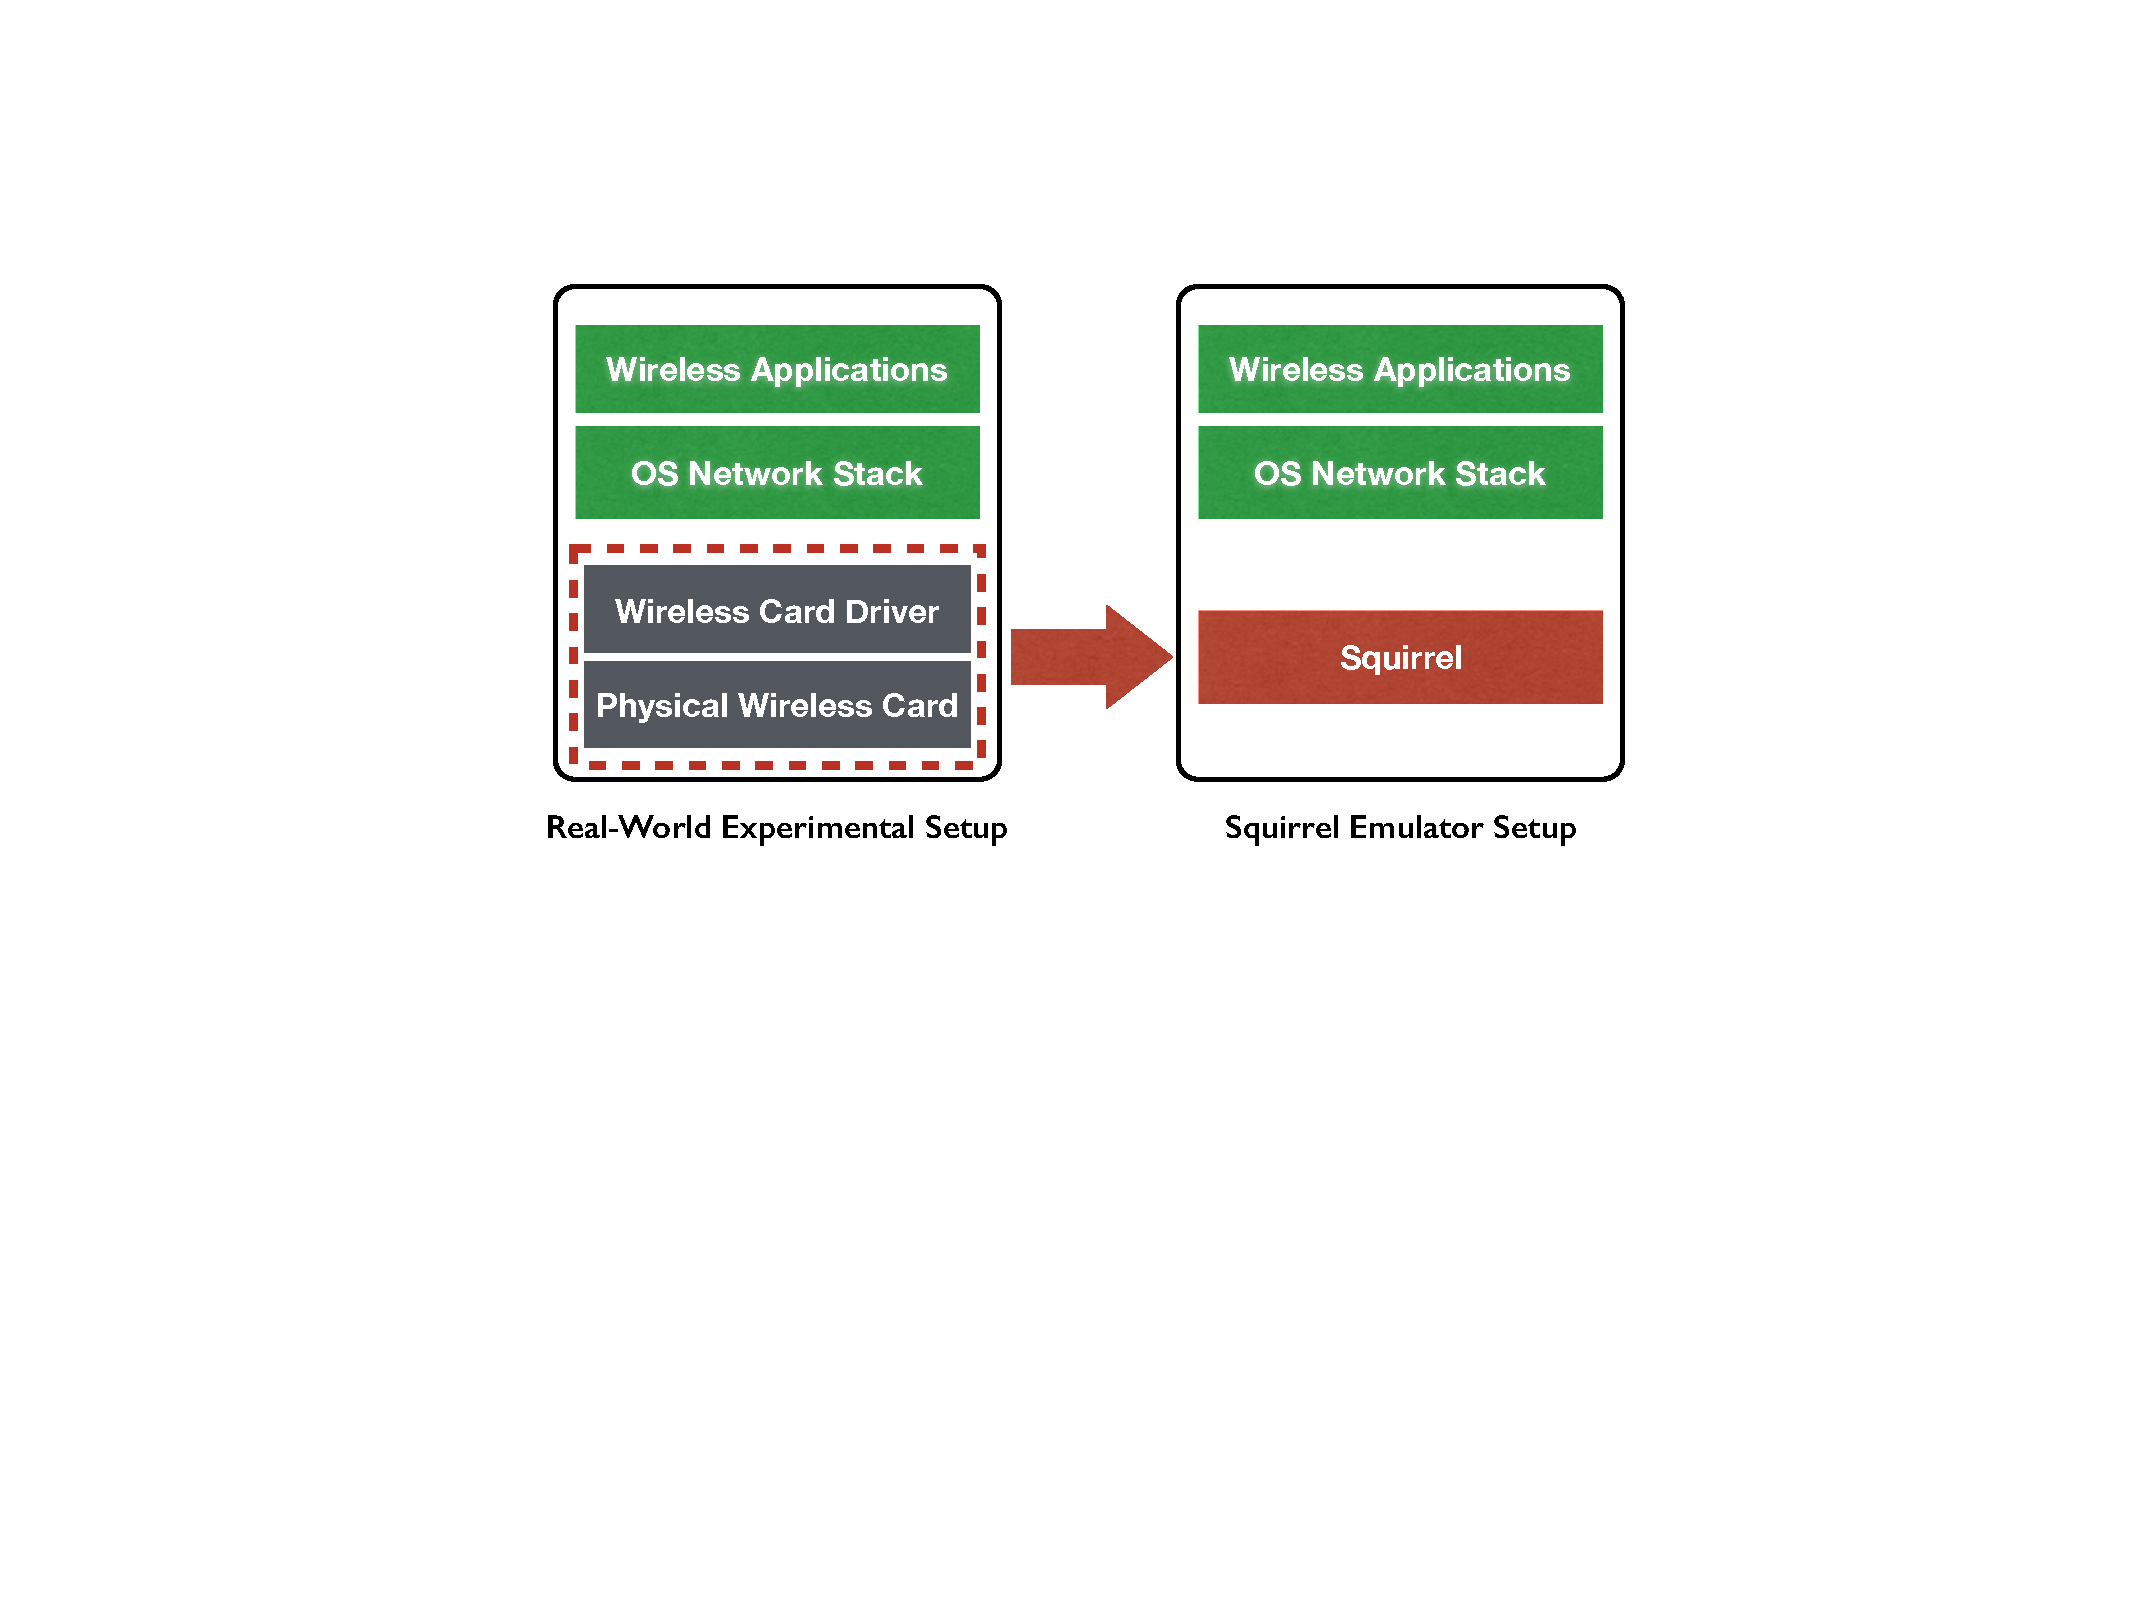
\includegraphics[width=.7\textwidth]{figures/squirrelConcept.pdf}
    \caption{\label{fig:squirrel_concept}Layer Concept of Squirrel}
  \end{center}
\end{figure}

\begin{figure}[h]
  \begin{center}
    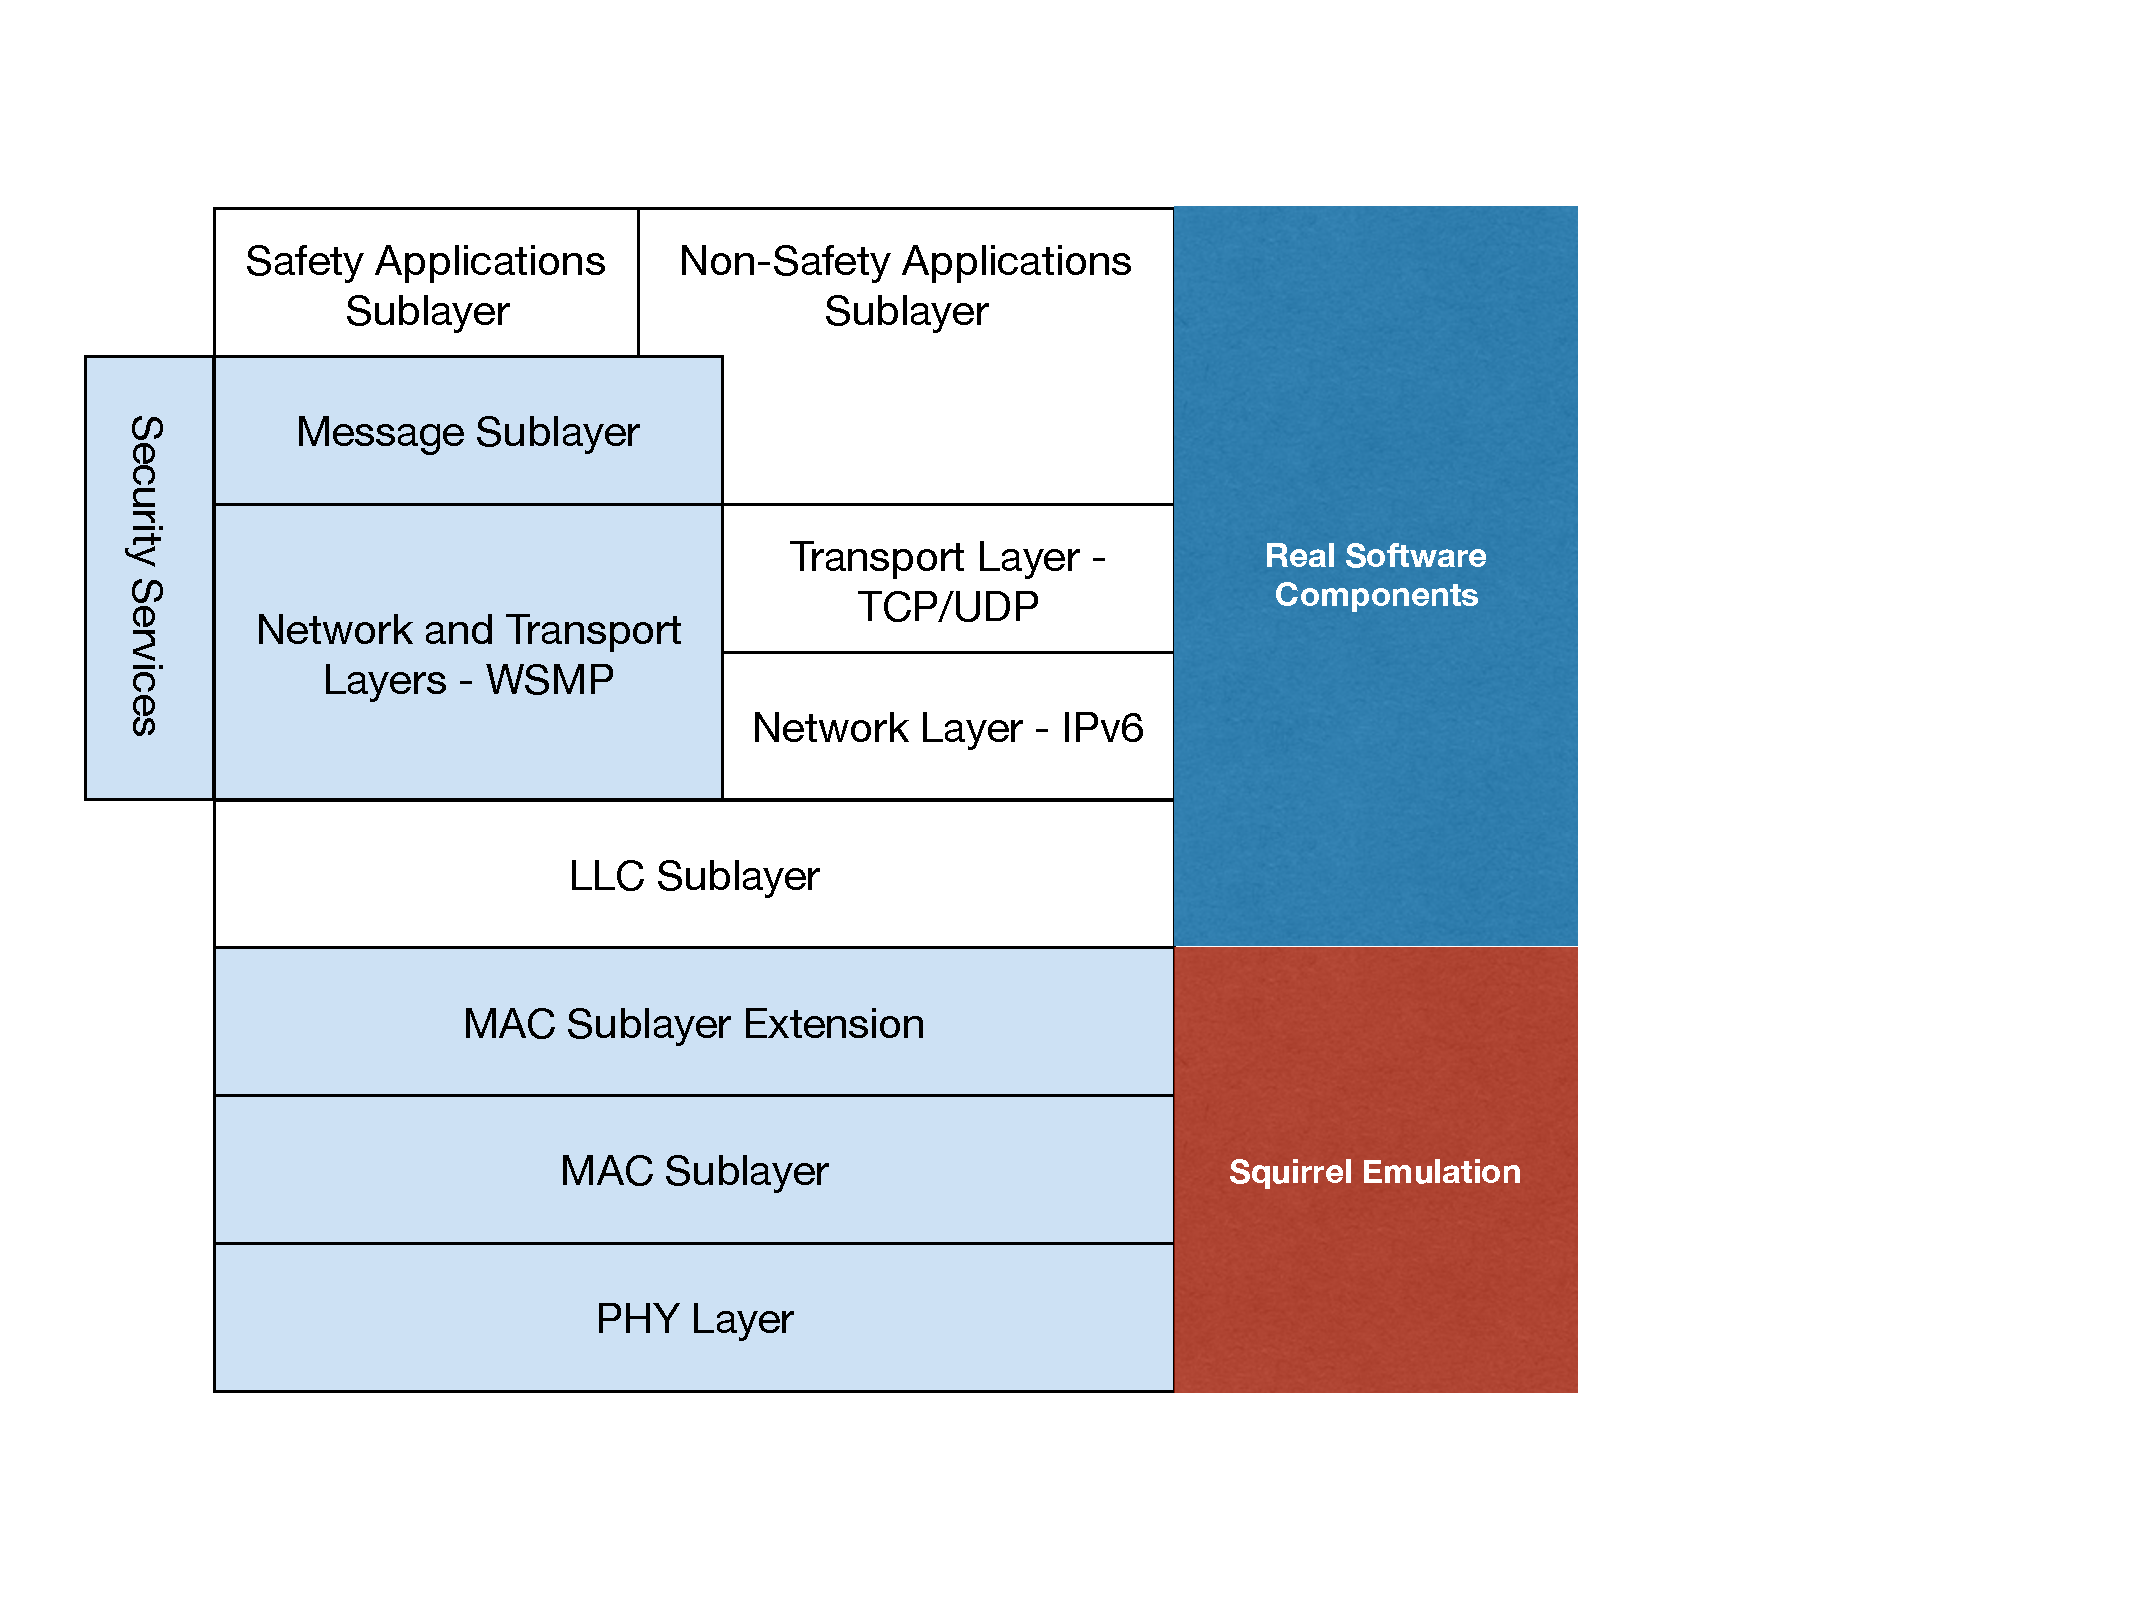
\includegraphics[width=.7\textwidth]{figures/squirrelDSRC.pdf}
    \caption{\label{fig:squirrel_dsrc}Squirrel in DSRC Context}
  \end{center}
\end{figure}

\subsection{Architecture}
Squirrel uses a multi-tier architecture, where a master component (\texttt{squirrel-master}) works as a server that coordinates communication among all participating nodes, and a worker component (\texttt{squirrel-worker}) that works as a client and handles communication details on actual nodes. There is only one \texttt{squirrel-master} in an emulation. It has an internal wireless model that determines whether data should be delivered on a frame-by-frame basis. The \texttt{squirrel-worker} component, on the other hand, has one instance running for each node being emulated. It connects the wireless components being tested with the \texttt{squirrel-master}, and handles the ``first mile" and ``last mile" of the network traffic.

\begin{figure}[h]
  \begin{center}
    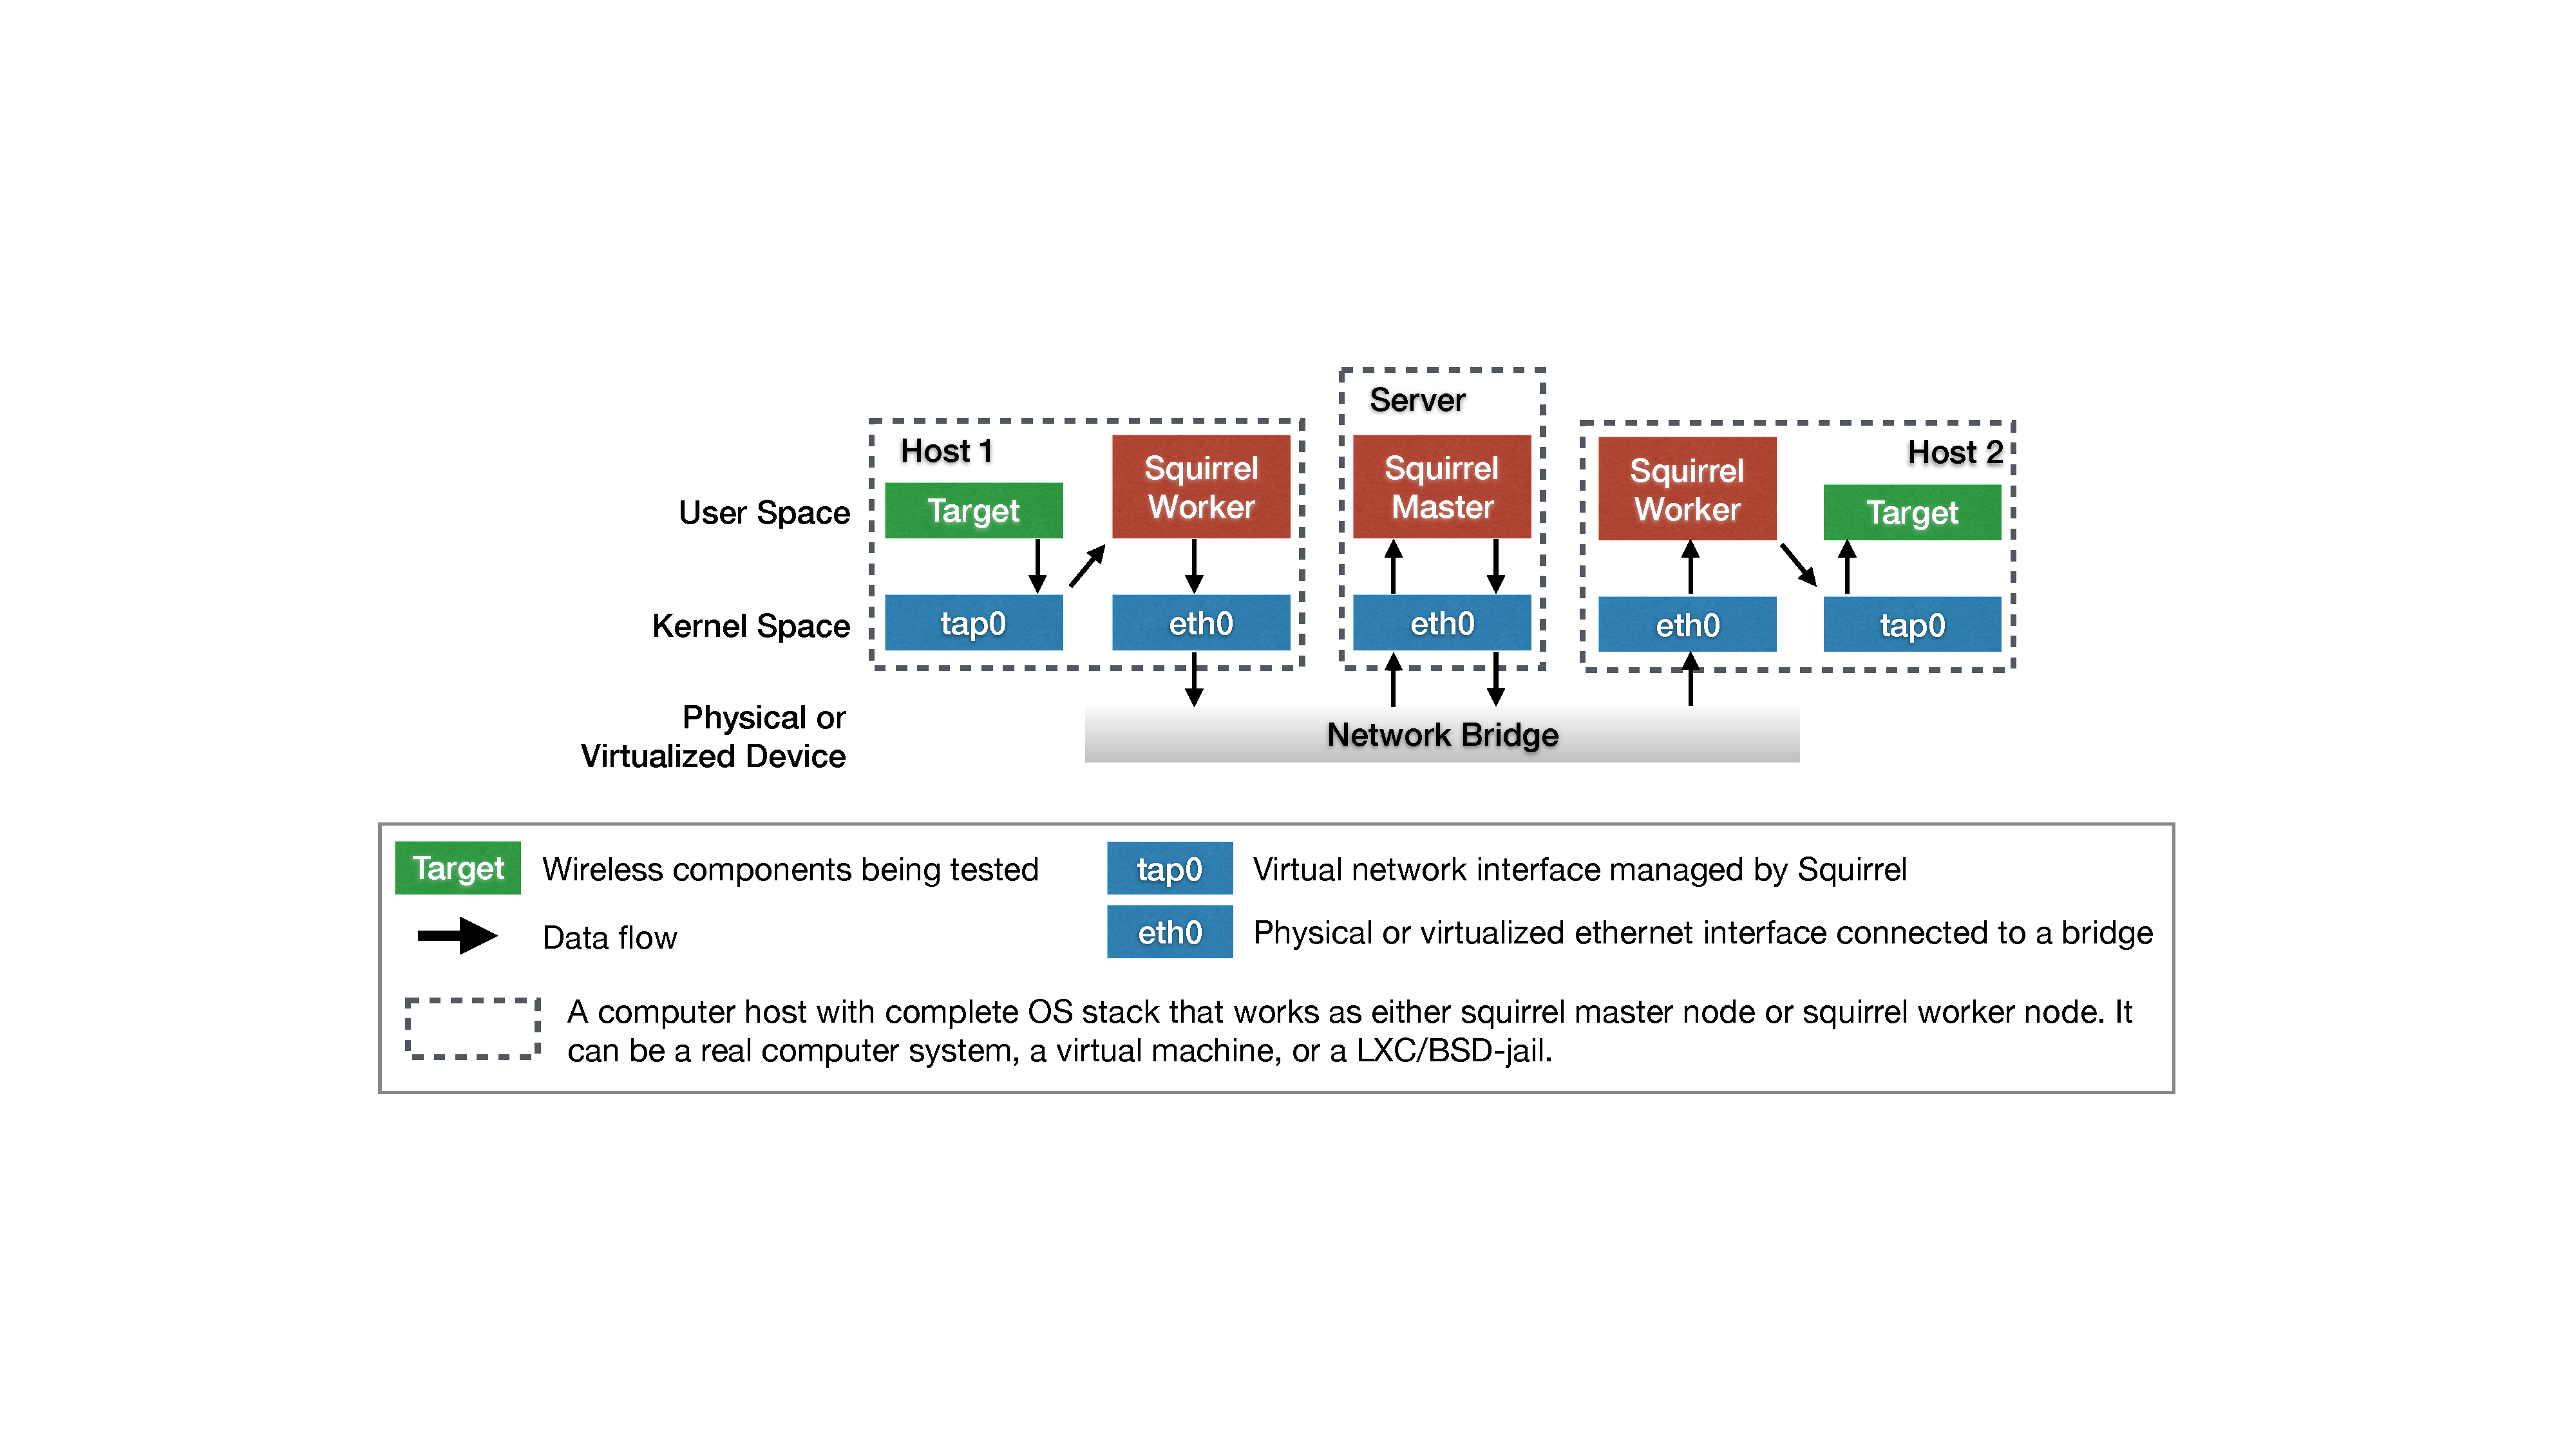
\includegraphics[width=\textwidth]{figures/squirrelArch.pdf}
    \caption{\label{fig:squirrel_arch}Squirrel Architecture and an Example Data Flow}
  \end{center}
\end{figure}

Figure~\ref{fig:squirrel_arch} illustrates the multi-tier architecture of Squirrel. Each host is a computer domain that has independent or isolated networking stack. It can represent a real computer system with independent hardware, a virtual machine, or an operating system level virtualization (OSLV\nomenclature{OSLV}{Operating System Level Virtualization}) host such as a Linux process container \cite{menage2007adding} and a BSD-jail. Among the three options, OSLV has the lowest overhead and is thus the most scalable. It allows different hosts to share a same operating system kernel and relies on the kernel namespace for isolating the filesystem and networking stack.

Squirrel uses a TAP\cite{tuntap2002} interface, \texttt{tap0} as in Figure~\ref{fig:squirrel_arch}, in each emulated wireless node as emulated wireless network interface. A TAP interface is a virtual network device that only exists in operating system kernels. It provides MAC layer frame reception and transmission for user space programs. From an application's perspective, the \texttt{tap0} interface can be seen as an Ethernet device, which, instead of receiving packets from a physical wireless network device, receives them from \texttt{squirrel-worker}, and instead of sending packets via a physical wireless network device, writes them to \texttt{squirrel-worker}. \texttt{squirrel-worker} has a file descriptor through which it can handle the \texttt{tap0} interface. Whenever an application writes any data into \texttt{tap0}, or any traffic is routed through the interface, \texttt{squirrel-worker} receives the data through the file descriptor. Whenever \texttt{squirrel-worker} writes into the file descriptor, a MAC frame is generated in kernel just like incoming traffic on a real device, and results in data received in the corresponding application.

\texttt{squirrel-worker} uses \texttt{eth0} interface to communicate with \texttt{squirrel-master}. This interface is not managed by Squirrel, but is an Ethernet interface managed by the operating system. If the emulated node is a real computer device, \texttt{eth0} is mapped to a real Ethernet adapter. If the emulated node is a virtual machine or OSLV host, it is a virtualized interface managed by the virtualization layer. Conceptually, this interface should be considered as an Ethernet interface that connects to \texttt{squirrel-master} either directly or through a Ethernet bridge. \texttt{eth0} is normally not used by testing targets directly, but an interface used by Squirrel to coordinate traffic. An exception is when the testing target needs to use an out-of-band channel to notify the \texttt{squirrel-master} about its local situation. For example, Section~\ref{sec:rpc_mobility_manager} describes a way to update emulated positions using RPC services, which runs on \texttt{eth0}.

An example data flow is also shown in Figure~\ref{fig:squirrel_arch}, where emulated node 1 (host 1) is sending data to emulated node 2 (host 2). The data flows from a testing target into \texttt{tap0}, which is read by \texttt{squirrel-worker} as MAC frames, and encapsulated into Squirrel's packet, then sent to \texttt{squirrel-master} through \texttt{eth0}. The \texttt{squirrel-master} upon receiving a frame, applies the wireless model and determines whether it should be delivered to the destination node. If so, it sends the frame packet to host 2, which is parsed into a MAC frame by \texttt{squirrel-worker}, and written into the \texttt{tap0} interface on host 2. The testing target then reads the data from \texttt{tap0} interface.

\texttt{squirrel-master} has two important components: a mobility manager and a wireless model. Both of them are configurable through a plug-in system. The two components share a position manager, which is an internal component in Squirrel that keeps track of position of each emulated node. The mobility manager emulates the mobility of all emulated nodes. It interfaces with the position manager and updates positions of emulated nodes periodically. The position information is used by the wireless model to determine whether a frame should be delivered to its destination.

During the development and testing of Squirrel, several simplified mobility managers and wireless models are developed. For example, a static mobility manager allows pre-definition of a position for each node. A PassThrough wireless model instructs Squirrel to deliver each frame. These models are useful for testing the effectiveness and capability of Squirrel, but do not provide realistic throughput and packet loss for application in emulation.

The rest of this section is focused on realistic models that are used in this study. First, a CSMA/CA wireless model is designed to emulate the CSMA/CA algorithm used in real-world IEEE 802.11 networks. Second, a mobility manager that supports updating positions from different processes is designed.

\subsection{CSMA/CA Model}
\label{sec:squirrel_csmaca}

In Ethernet, the collision domain is bounded to well controlled hardware components such as Ethernet wires and hubs. In wireless networking, however, since electro-magnetic wave propagates freely, the collision domain is much larger and the bounds are less pronounced. This introduces some challenges specific for wireless networking. A typical one is the hidden node problem, where a node transmitting to a second node may not see other nodes that are in interference range of the second node but not the first one, causing collision at second node. This is the motivation that lead to the design of collision avoidance in CSMA/CA algorithm that is widely used in IEEE 802.11 networks.

\begin{figure}[h]
  \begin{center}
    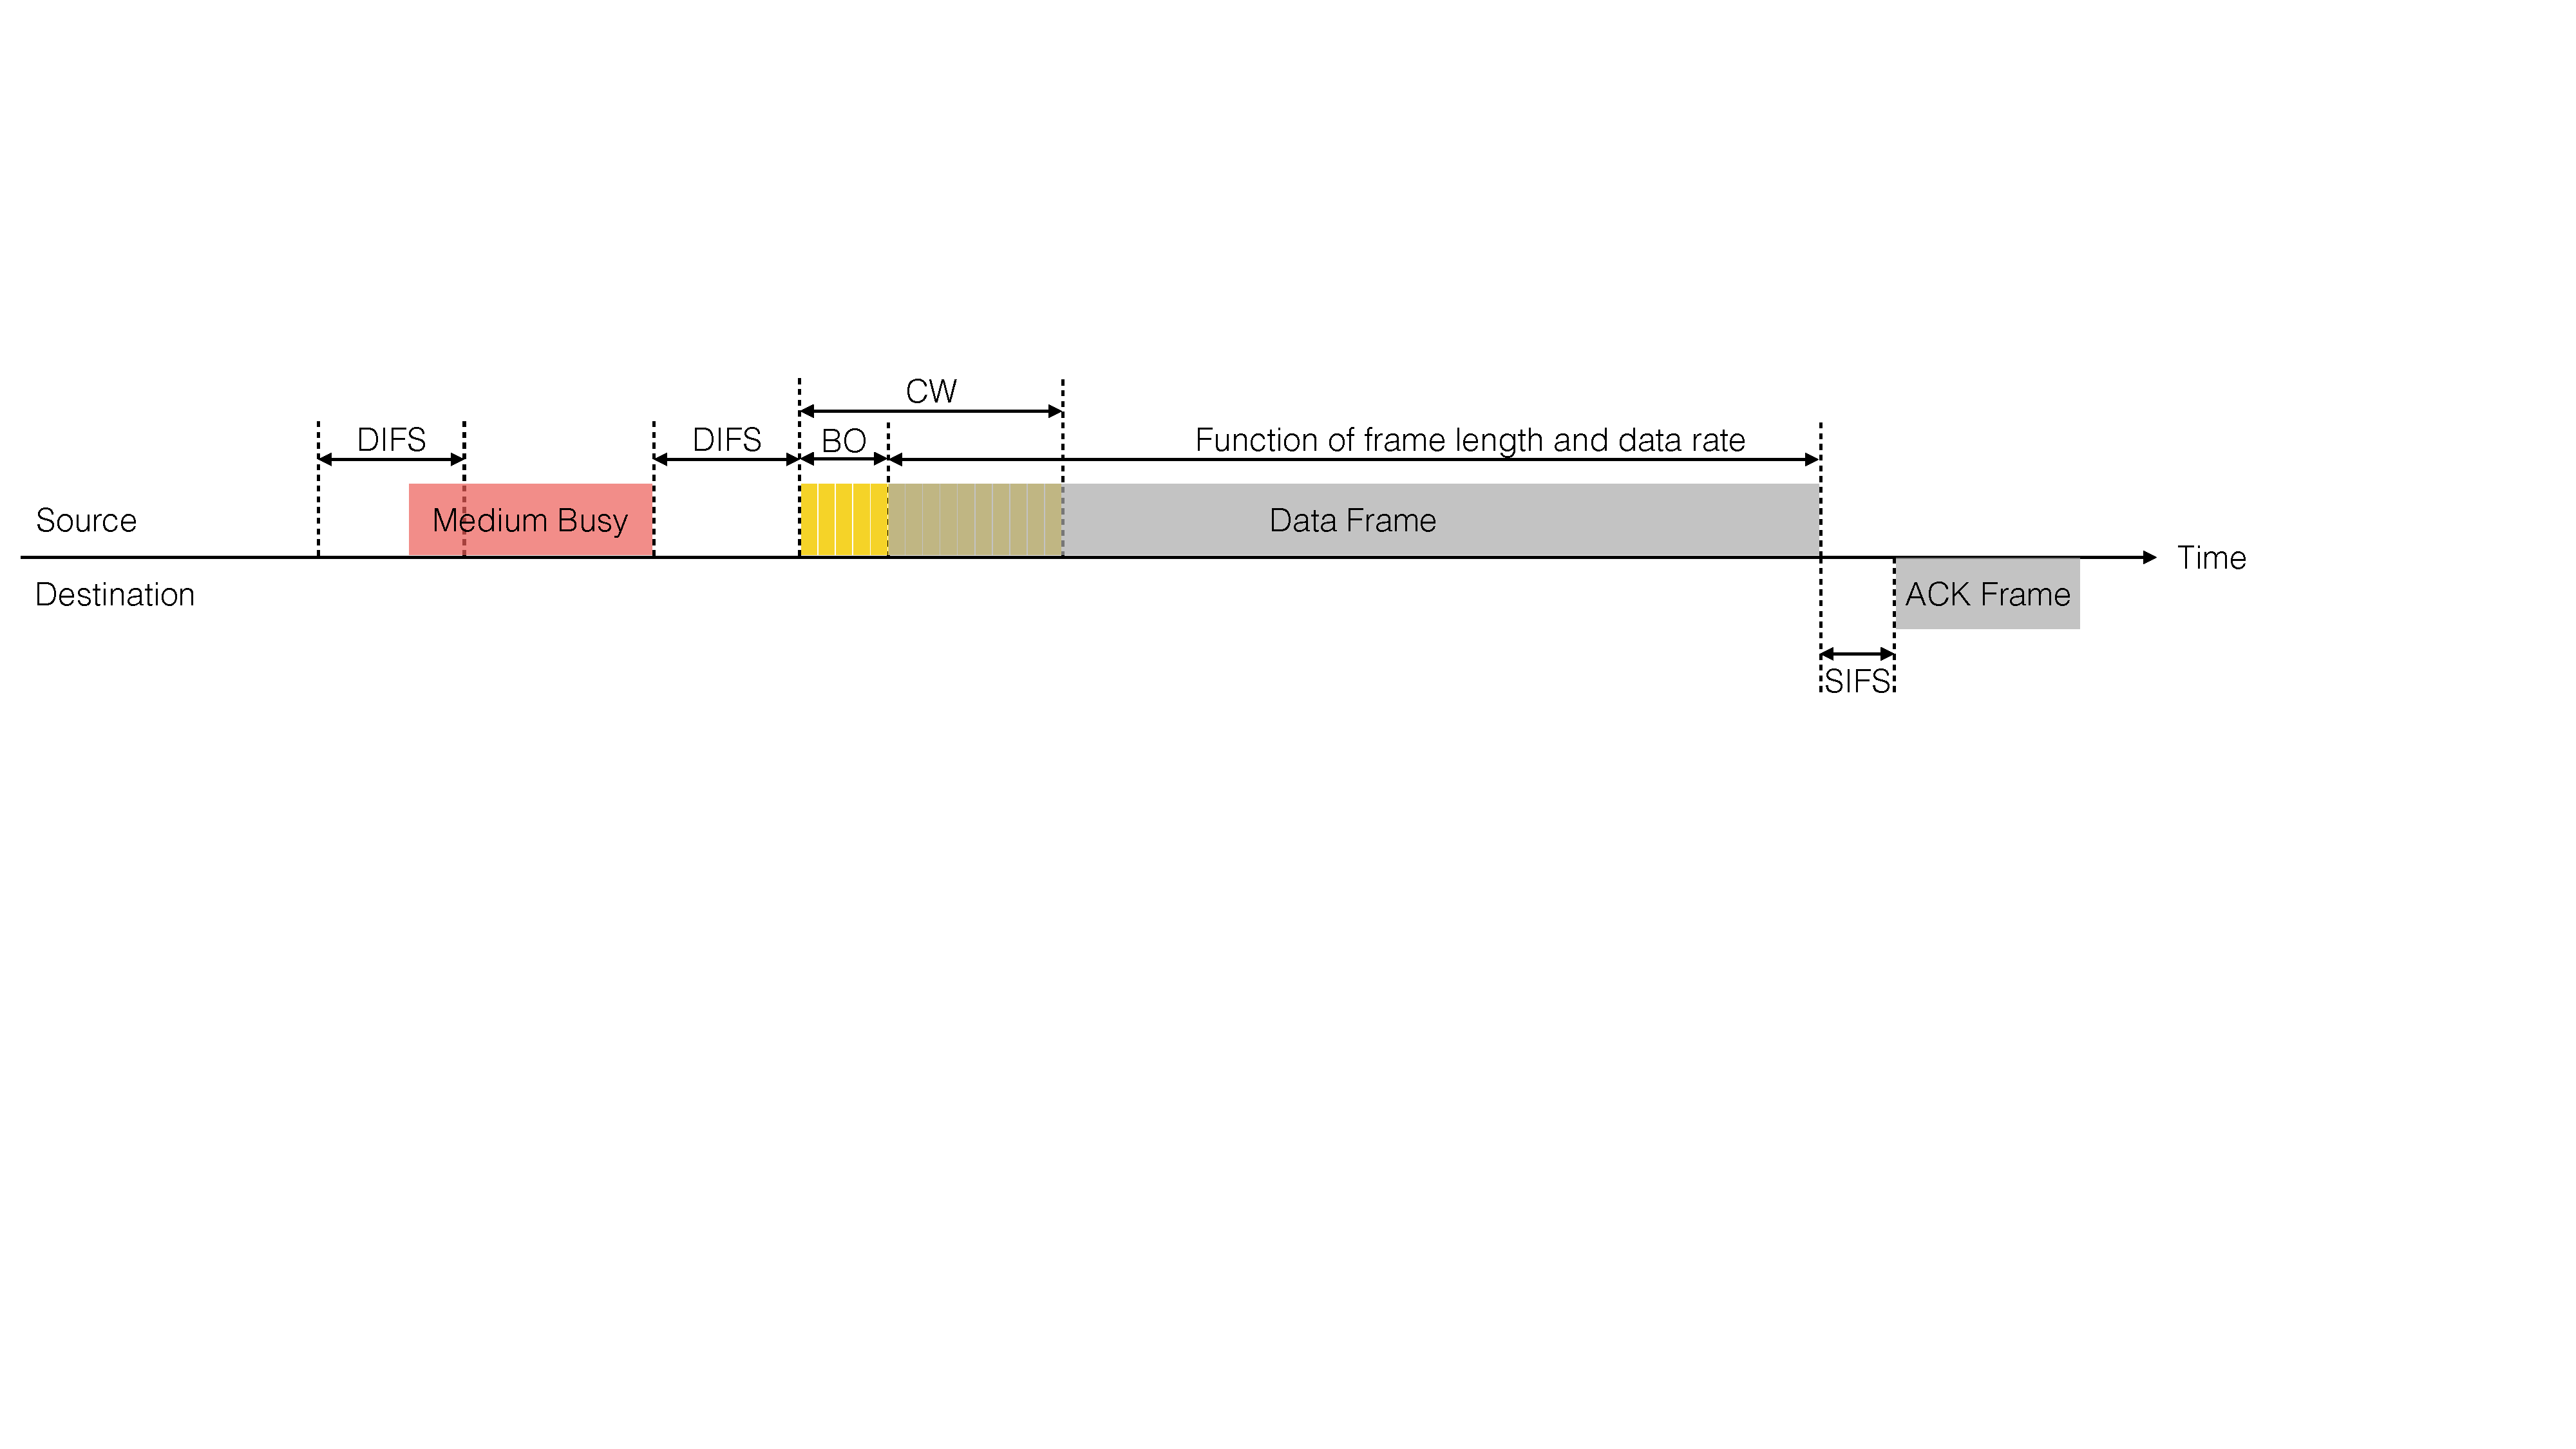
\includegraphics[width=\textwidth]{figures/csmaca.pdf}
    \caption{\label{fig:csmaca}A CSMA/CA Algorithm Timeline of Sending a Data Frame}
  \end{center}
\end{figure}

Figure~\ref{fig:csmaca} shows a typical timeline of sending a data frame CSMA/CA algorithm. In CSMA/CA, when a node needs to transmit a data frame, it first senses the medium, i.e., the wireless channel. When the channel has been idle for a predefined period of time, Distributed coordination function Inter-Frame Space (DIFS\nomenclature{DIFS}{Distributed coordination function Inter-Frame Space}), it starts a random Back-Off time counter (BO\nomenclature{BO}{Back-Off time counter}), which is equal to a number of $aSlotTime$ within Contention Window (CW\nomenclature{CW}{Contention Window}). The counter decrements when the medium is idle. When BO hits zero, the data frame is transmitted. If this is a broadcast frame, that is the end of cycle for this frame. If this is a unicast frame, when the frame is successfully received at destination, the destination node waits for Short Inter-Frame Space (SIFS\nomenclature{SIFS}{Short Inter-Frame Space}), which is shorter than DIFS, and then transmits an Acknowledgement Frame (ACK\nomenclature{ACK}{Acknowledge Frame}). The ACK allows the source node to be notified about the reception of the frame at destination node. If a frame is lost, the source retransmits the frame, and at the same time, increases the CW. When a frame is successfully transmitted, CW is reset to lowest value. Following this process, the time it takes to typically transmit a data frame, $T_{data}$, can be modeled with Equation~\ref{eq:csmaca_send_data}:

\begin{equation}
  T_{data}=t_{busy}+t_{DIFS}+t_{BO}\times aSlotTime+t_{data}
  \label{eq:csmaca_send_data}
\end{equation}

where $t_{busy}$ is the time duration that the channel is busy, including partial DIFS's, as well as busy time during BO, and $t_{data}$ is the time duration it takes to encode the actual data frame. The time it takes to transmit an ACK, $T_{ACK}$, can be modeled with Equation~\ref{eq:csmaca_send_ack}:

\begin{equation}
  T_{ACK}=t_{SIFS}+t_{ACK}
  \label{eq:csmaca_send_ack}
\end{equation}

where $t_{ACK}$ is the time duration it takes to encode the actual ACK.

In IEEE 802.11 protocols, DIFS is defined as $SIFS + 2 \times aSlotTime$. In IEEE 802.11p with 10MHz channel, SIFS is defined to be 13 microseconds, and $aSlotTime$ is defined as 32 microseconds. CW's lowest value is 15, and the maximum that CW can grow into is 1023. \cite{ieee201280211macphy}

Unlike in the real-world, where the CSMA/CA algorithm can rely on network adapter to sense whether channel is available to use, in emulation, the model needs to approximately keep track of localized channel condition of each node. To be more specific, it needs to keep track of how much of the channel time is being used in the vicinity of each node being emulated. When a node needs to transmit, or when other nodes need to transmit to the node, the model needs to check the channel condition around this node, and determines whether the channel is available for the data to be delivered. This is achieved by using the leaky bucket algorithm.

Leaky bucket algorithm \cite{turner1986,yin1991} is commonly used in networking to shape and/or enforce throughput. The idea is to have a counter, i.e., the bucket, that is incremented whenever a packet goes through, and is decremented periodically. If the counter exceeds a threshold upon being incremented, the network discards the packet. The rate at which the counter is decremented determines the average bandwidth. Figure~\ref{fig:leaky_bucket} shows the leaky bucket analogy.

\begin{figure}[h]
  \begin{center}
    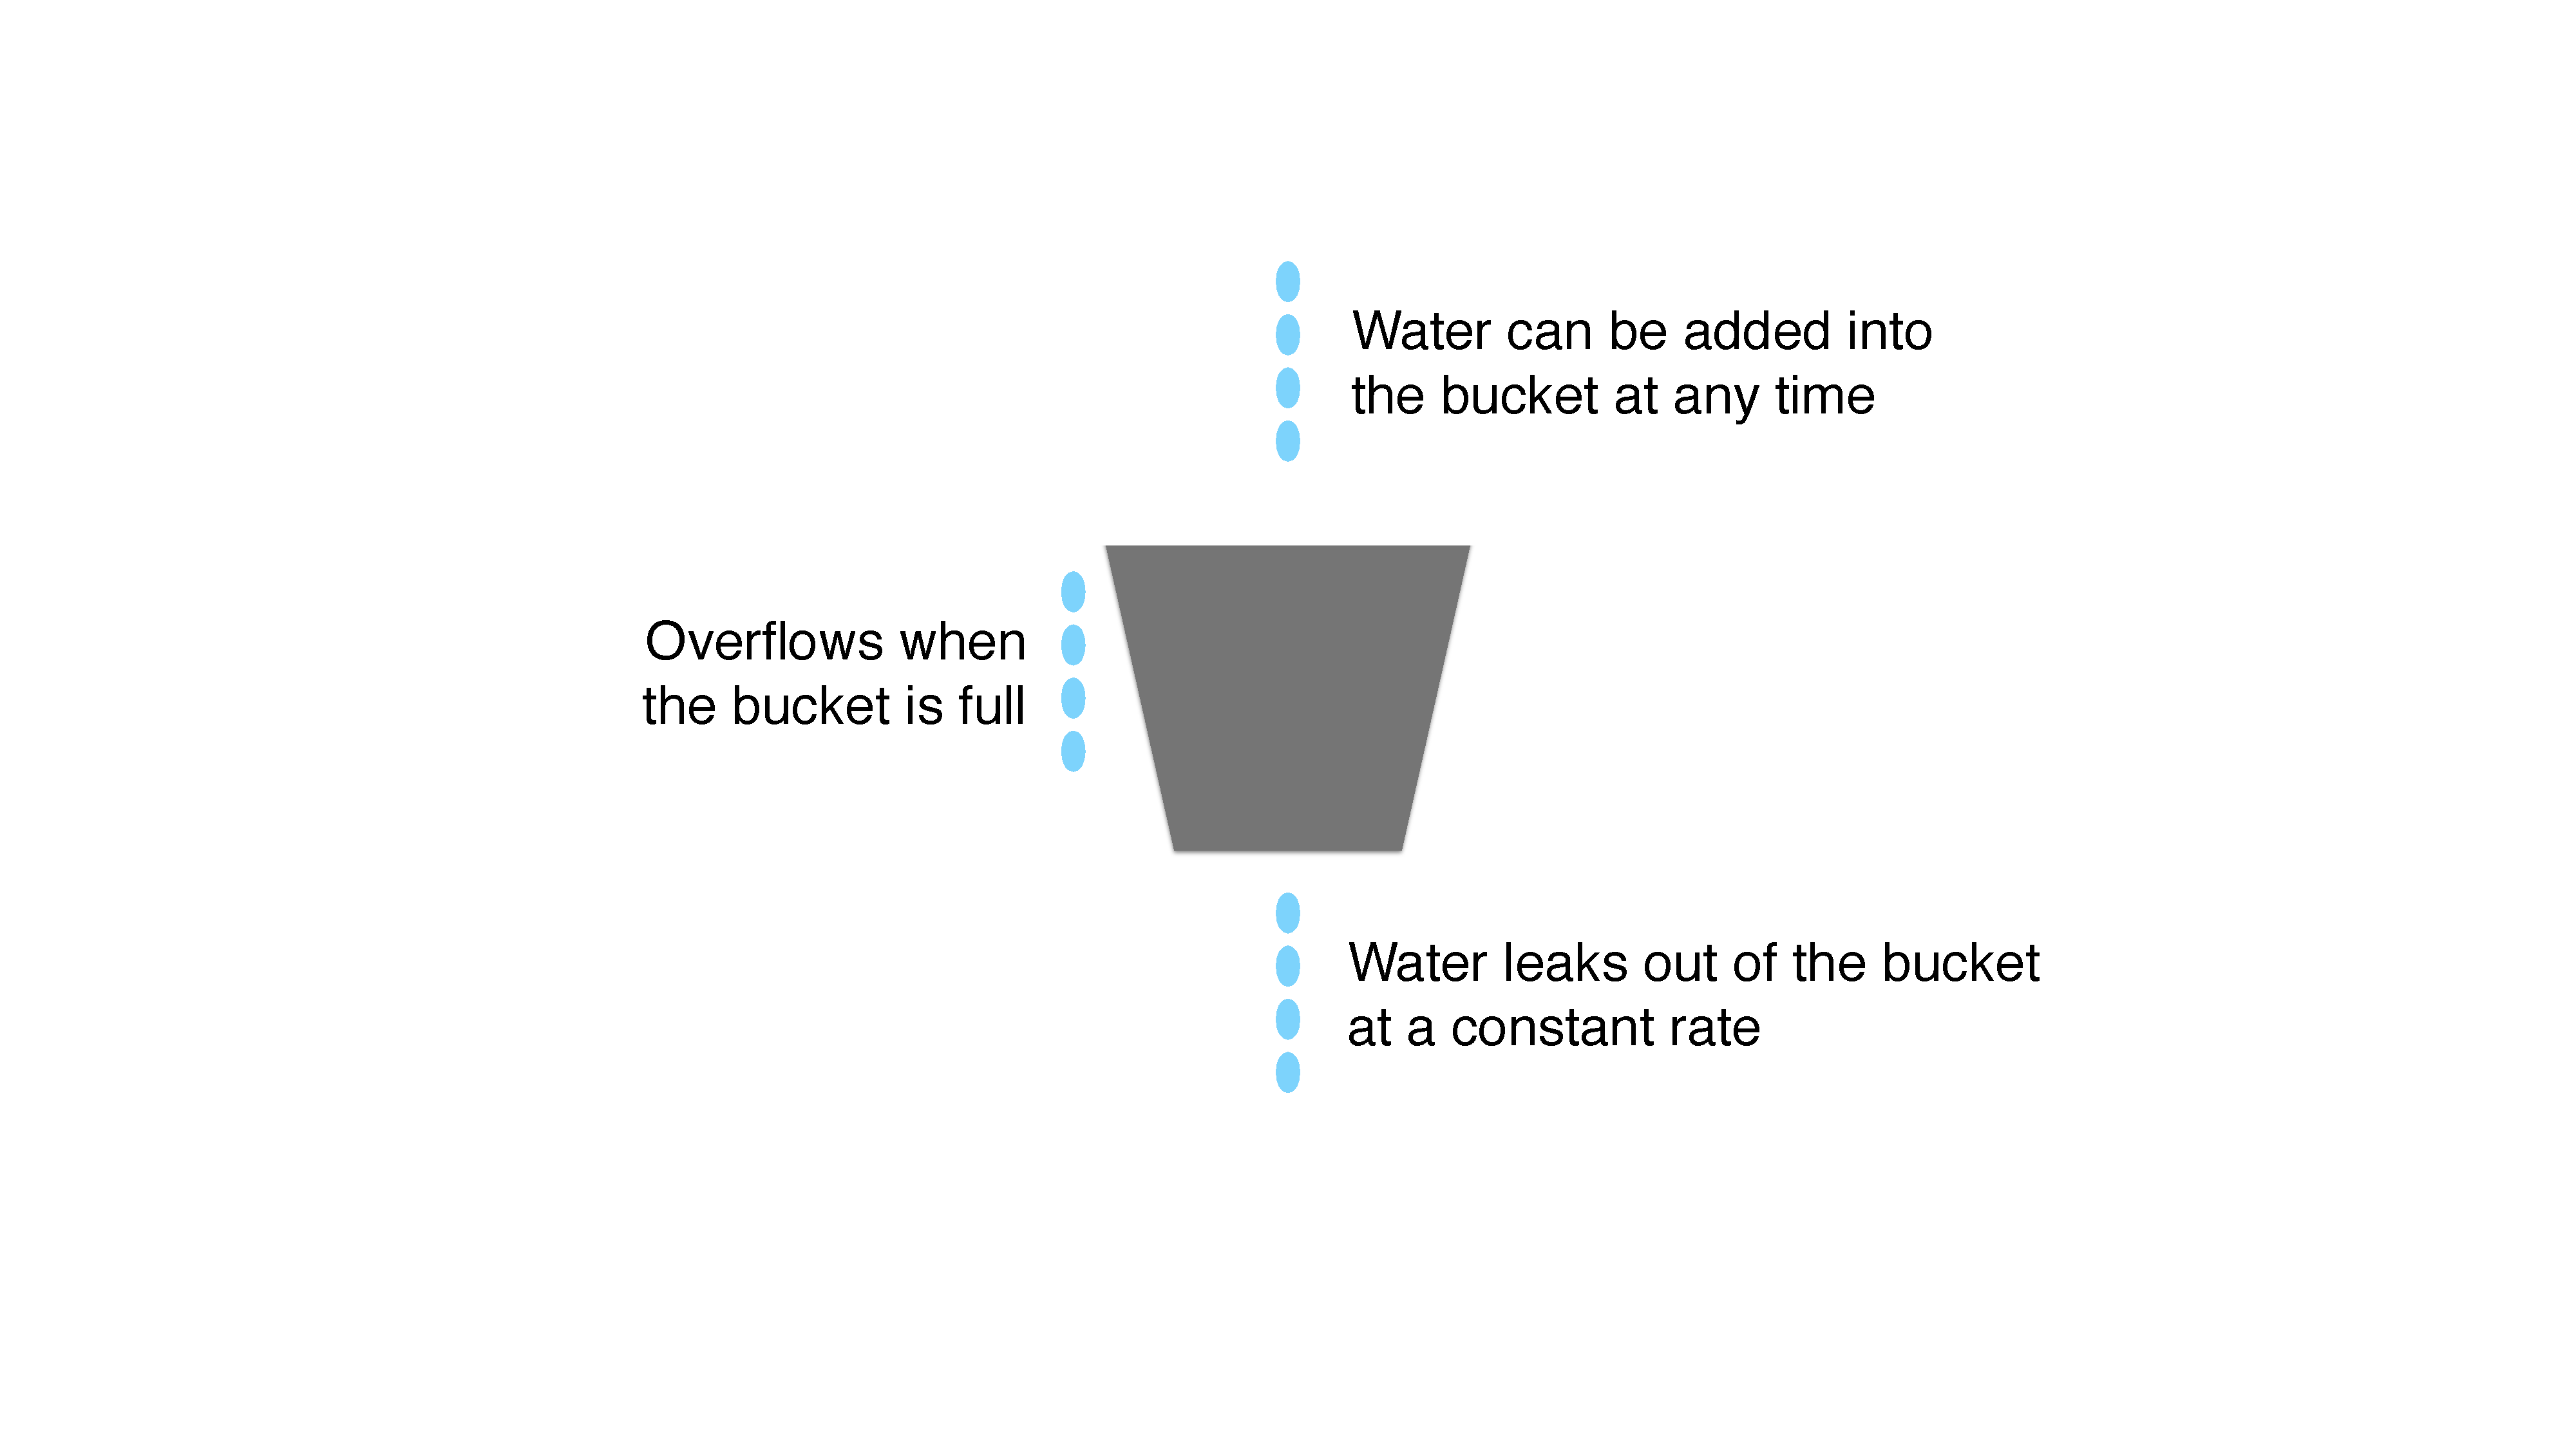
\includegraphics[width=.6\textwidth]{figures/leakyBucket.pdf}
    \caption{\label{fig:leaky_bucket}The leaky bucket analogy}
  \end{center}
\end{figure}

In Squirrel's IEEE 802.11 model, one leaky bucket is allocated for each node to track the channel condition around the node. The unit used for the counter is nanosecond. The rate at which the bucket leaks, i.e., counter decrements, is as same as the rate at which time elapses, i.e. $1\times 10^9$ per second. The counter is increased whenever an event happens, and the amount it increases is the time it takes for the event to happen. When the bucket is full, it indicates that the channel is congested around the corresponding node, and no more frames can be delivered to the node or sent from the node at the time.

Tracking channel condition with leaky buckets takes care of the process of ``carrier sensing". As a result, in the emulation model, nodes do not actually sense the medium, but starts DIFS and BO directly for each transmitting frame. This eliminates the $t_{busy}$ in Equation~\ref{eq:csmaca_send_data}. So the equation for calculating time duration to transmit a data frame $T_{data}$ in the emulation model is Equation~\ref{eq:csmaca_squirrel_send_data}:

\begin{equation}
  T_{data}=t_{DIFS}+\frac{t_{cw}}{2}\times aSlotTime+t_{data}
  \label{eq:csmaca_squirrel_send_data}
\end{equation}

where $t_{cw}$ is the current effective CW. Since BO is uniformly distributed in $[0,CW]$, $\frac{t_{cw}}{2}$ is used as BO here to reduce time complexity of the model. Equation for calculating time duration to transmit an ACK remains the same as Equation~\ref{eq:csmaca_send_ack}.

In addition to the leaky buckets, Squirrel's CSMA/CA model also uses a probability function $P_{propagation}$ to model the process of propagation of electro-magnetic wave. The probability function, as defined in Equation~\ref{eq:propagation_prob}, is based on the distance between source and destination nodes, as well as channel occupancy level, i.e., how full the bucket is.

\begin{equation}
  P_{propagation}=((1-u) * 0.1 + 0.9) * (1-(\frac{d}{r})^3)
  \label{eq:propagation_prob}
\end{equation}

where $u(0\le u\le 1)$is the usage ratio of the bucket, $d$ is the distance between source and destination nodes, and $r$ is the transmission range.

Putting it together, when a node transmits a unicast data frame, Squirrel's CSMA/CA model first tries to increment the bucket of the source node. If successful, it tries to increment all buckets within the interference range of the source node, based on Equation~\ref{eq:csmaca_squirrel_send_data}. If the destination bucket does not overflow, the probability function $P_{propagation}$ as defined in Equation~\ref{eq:propagation_prob} is applied. If the frame survives the probability function, the frame is delivered to the destination node. Any failure in this process results in retransmission, until the maximum number of transmission is reached. If the data frame is delivered to the destination node, the model starts the ACK process in which the destination node sends an ACK back to source node. This is a similar process, which includes incrementing buckets of nearby nodes, as well as the probability function. Although at this point, the data frame is for sure delivered to the destination node, the ACK can still be lost, in which case a retransmission still happens. Broadcast frames are handled in the same way, except that the model tries to deliver the data frame to all nodes within transmission range, and that there is not ACK process.

The CSMA/CA has configurable parameters, such as emulated MAC layer data rate, transmission range, and interference range. In addition, since different IEEE 802.11 protocol has different timing parameters, such as DIFS, SIFS, and aSlotTime, the CSMA/CA model has a configuration field for MAC layer protocol. The CSMA/CA model has a pre-defined parameter set for each supported protocol, which configures corresponding timing parameters for the model. An example of such parameter set is \texttt{802.11p10}, or \texttt{OFDM10}, which is configured to have 13 ms aSlotTime, 32 ms SIFS, and CW from 15 to 1023.


\subsection{RPC Updated Mobility Manager}
\label{sec:rpc_mobility_manager}

There are two approaches to design a mobility manager. The most straightforward way is to have a mobility model within the mobility manager, which emits new positions for emulated nodes based on the mobility model. This approach is useful for studying a specific mobility pattern, such as random waypoint, that can be easily well modeled with equations and software programs. Another approach is to follow an external trace which consists of a time series position data for each node, and update positions for emulated nodes accordingly. This approach provides a way to utilize external mobility simulators, or trace files from real-world experiments.

In this study, we acquired some real-world test traces. To produce most realistic results, the second approach is used. A Remote Procedure Call (RPC\nomenclature{RPC}{Remote Procedure Call}) updated mobility manager is designed. The mobility manager uses gRPC \cite{grpc} protocol. It includes a server that exposes several RPC services that allows a different process to update positions for emulated nodes. As opposed to directly reading from a trace file, the RPC updated mobility manager delegates the work or interpreting trace files to a different process. This provides flexibility on trace file formats. In addition, in many cases, trace files include many types of data including GPS positions, DSRC send and receive history, etc.. The RPC updated mobility manager allows a dedicated process to replay all relevant events. This is used by \texttt{truck-playback}, which is described in Section~\ref{sec:truck_playback}.

To make sure the RPC services do not affect the CSMA/CA model's results, the RPC Updated Mobility Manager is only used through the \texttt{eth0} interface.

\section{Implementation}
\label{sec:squirrel_implementation}

Squirrel and its components are implemented in Go programming language \cite{golang}. The language is chosen because of its good balance between safety, development efficiency, and performance. Designed as a system language, Go has well designed support for system software, such as first-class concurrency, well-designed networking APIs and system call interface, and cross-compile tools. These features benefit the development of Squirrel, resulting in stability and high performance\footnote{An earlier version of the emulator was developed using C++ with \texttt{Boost.Asio}, which achieved only about half throughput of that in the Go version.}.

Despite the advantages, Go provides less control over memory management of the applications compared to other system languages such as C/C++. The garbage collection takes care of reclaiming memory no longer used, so a straightforward way to code is to allocate new objects whenever needed, and let the garbage collection worry about freeing the memory. This approach works in most cases. However for Squirrel's use case, packets are generated and consumed at very high rate, which results in byte buffers of same size allocated and deallocated frequently. The allocation and deallocation increases processing burden and is inefficient. In Squirrel, a buffer pool is used for reusing existing byte buffers, using the free-list data structure. In addition, the buffer pool implements a thread-safe reference counting, similar to \texttt{std::shared\_ptr} in C++, to allow multiple components share the same object, and reuse objects at precisely the time when they are not needed.

Squirrel has many configurable parameters. For example, the plug-in system allows different wireless models and mobility managers to be selected. The wireless models and mobility managers have their own parameters as well, such as data rate and interference range in CSMA/CA, and RPC service endpoint address of the RPC Updated Mobility Manager. Besides parameters, the \texttt{squirrel-master} needs to announce its endpoint address once it has started, so \texttt{squirrel-worker}s can connect to it. For these dynamic configurations, a fast and reliable distributed key-value store, Etcd \cite{etcd}, is used. It uses the Raft consensus algorithm \cite{ongaro2014search} to manage a highly-available replicated log, which supports running multiple Etcd instances forming a cluster, to improve reliability and availability.

Since every frame goes through \texttt{squirrel-master}, it can easily become a bottleneck for the entire emulation infrastructure. Hence, it is important to optimize \texttt{squirrel-master} in a way that it is scalable by deploying it on a machine with more processing power and more simultaneous running threads. With this goal, \texttt{squirrel-master} uses a lock-free design whenever possible. For example, in the CSMA/CA model, the leaky bucket is implemented with \texttt{sync/atomic} package, using atomic operations that do not require a Mutex to guard resources. The position manager uses fine-grain locking mechanism, where accessing thread only blocks when read and write, or write and write happen for the same node's position at the same time. This design makes \texttt{squirrel-master} more parallelization friendly, thus scales better on multi-core systems.

\section{Tests}

\subsection{Effectiveness Test}

To validate that Squirrel provides networking service for applications comparable with real-world scenarios, some tests are conducted to run the same traffic on real-world WiFi devices and Squirrel.

There are four nodes involved in the tests. In Android configuration, the four nodes are connected to an Ad-Hoc WiFi network at 2.4 GHz, placed right next to each other, with distance less than 100 millimeters. In the Squirrel configuration, CSMA/CA wireless model is used, with the four emulated nodes placed 150 units from each other. Communication range is set to 150,000 units and interference range is set to 300,000. In other words, in both configurations the nodes are very close to each other so that interference rather than distance is the major affecting factor to wireless performance.

A simple networking testing tool, \texttt{iperf}, is used as testing target. UDP traffic is used since it does not have congestion control and gives a good perception of above-MAC-layer throughput. Two pairs of \texttt{iperf} tests are run, between two different pairs of nodes. The first pair (node1 to node2) starts first. It is set to run for 30 seconds. The second pair (node3 to node4) starts when the first has started for 10 seconds, and runs for 10 seconds. This way, during the first and last 10 seconds, only one pair of nodes are transmitting, while from 10th second and 20th second, both pairs are transmitting.

\begin{figure}[h]
  \begin{center}
    \begin{subfigure}[h]{\textwidth}
      \makebox[\textwidth][c]{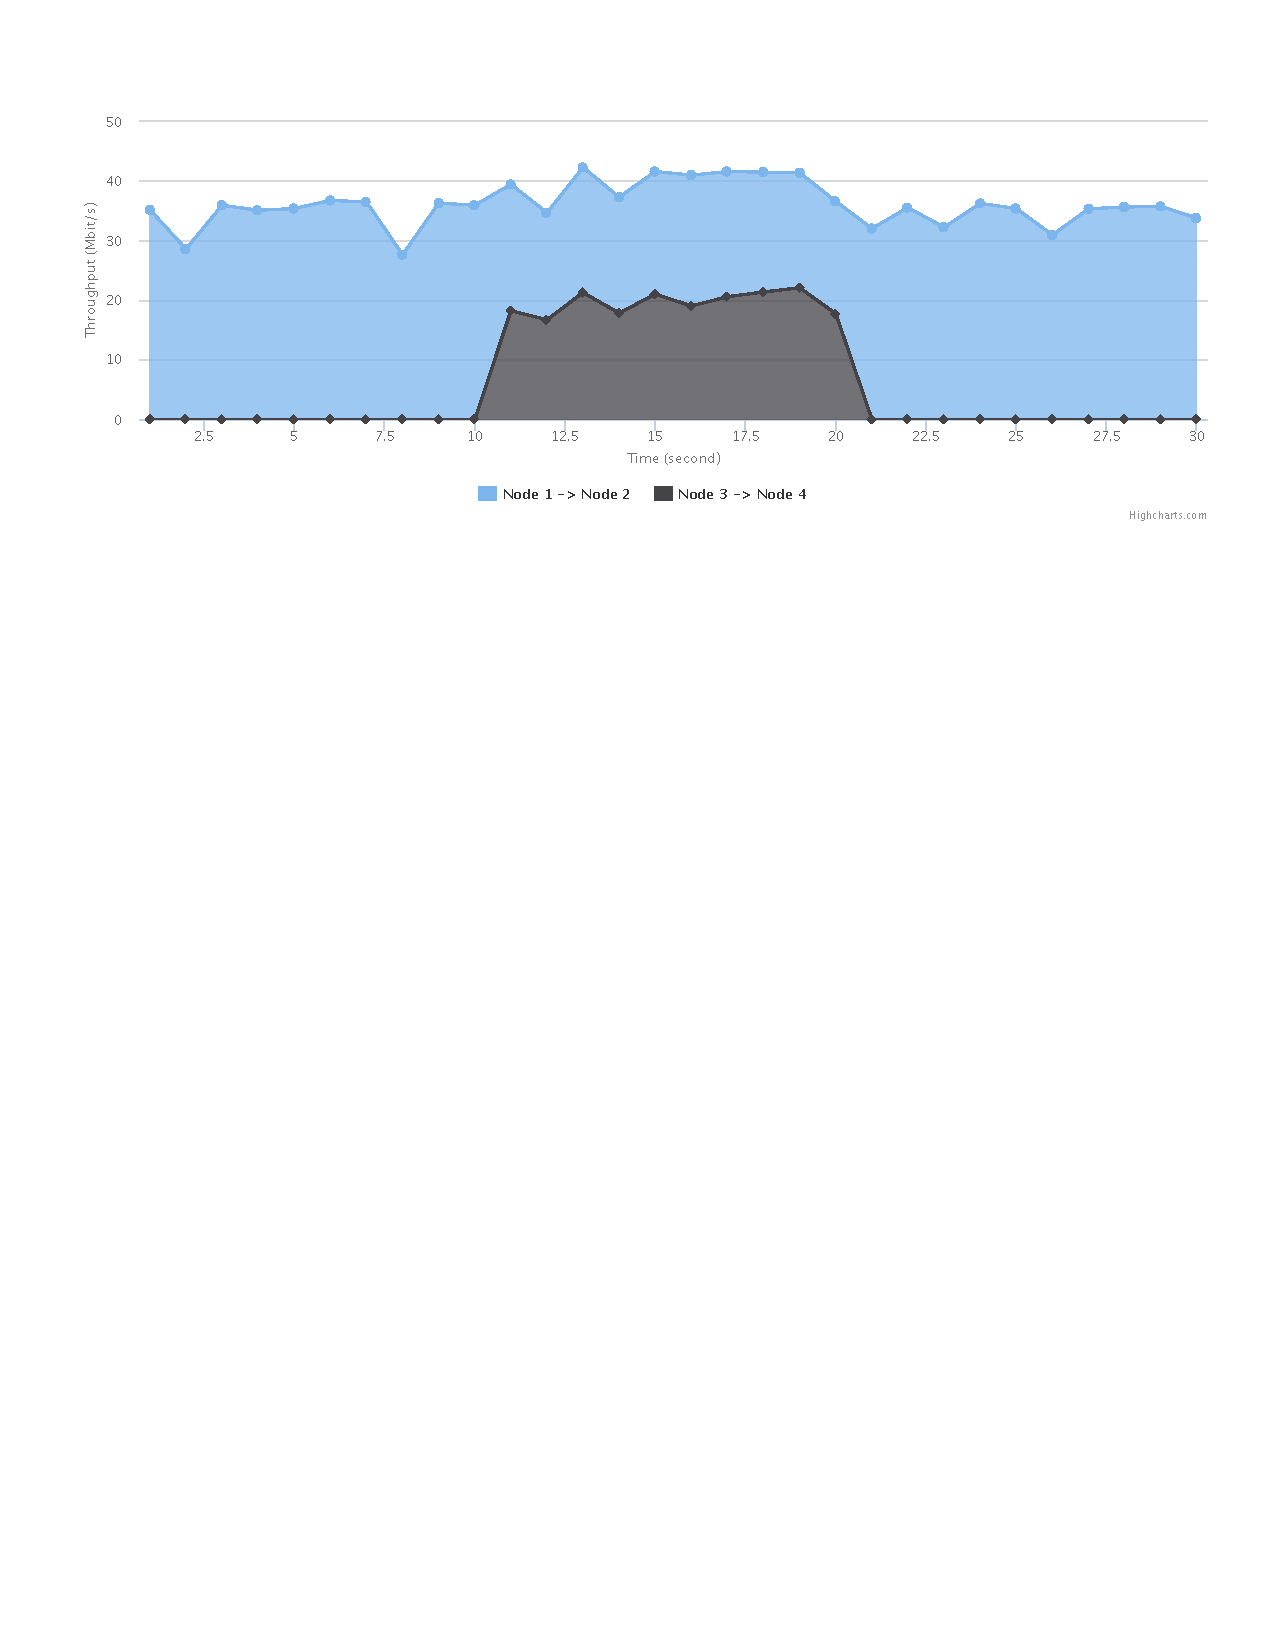
\includegraphics[width=1.1\textwidth]{figures/results/effectiveness_android.pdf}}
      \caption{\label{fig:squirrel_preliminary_android}Real Android UDP Throughput}
    \end{subfigure}
    \begin{subfigure}[h]{\textwidth}
      \makebox[\textwidth][c]{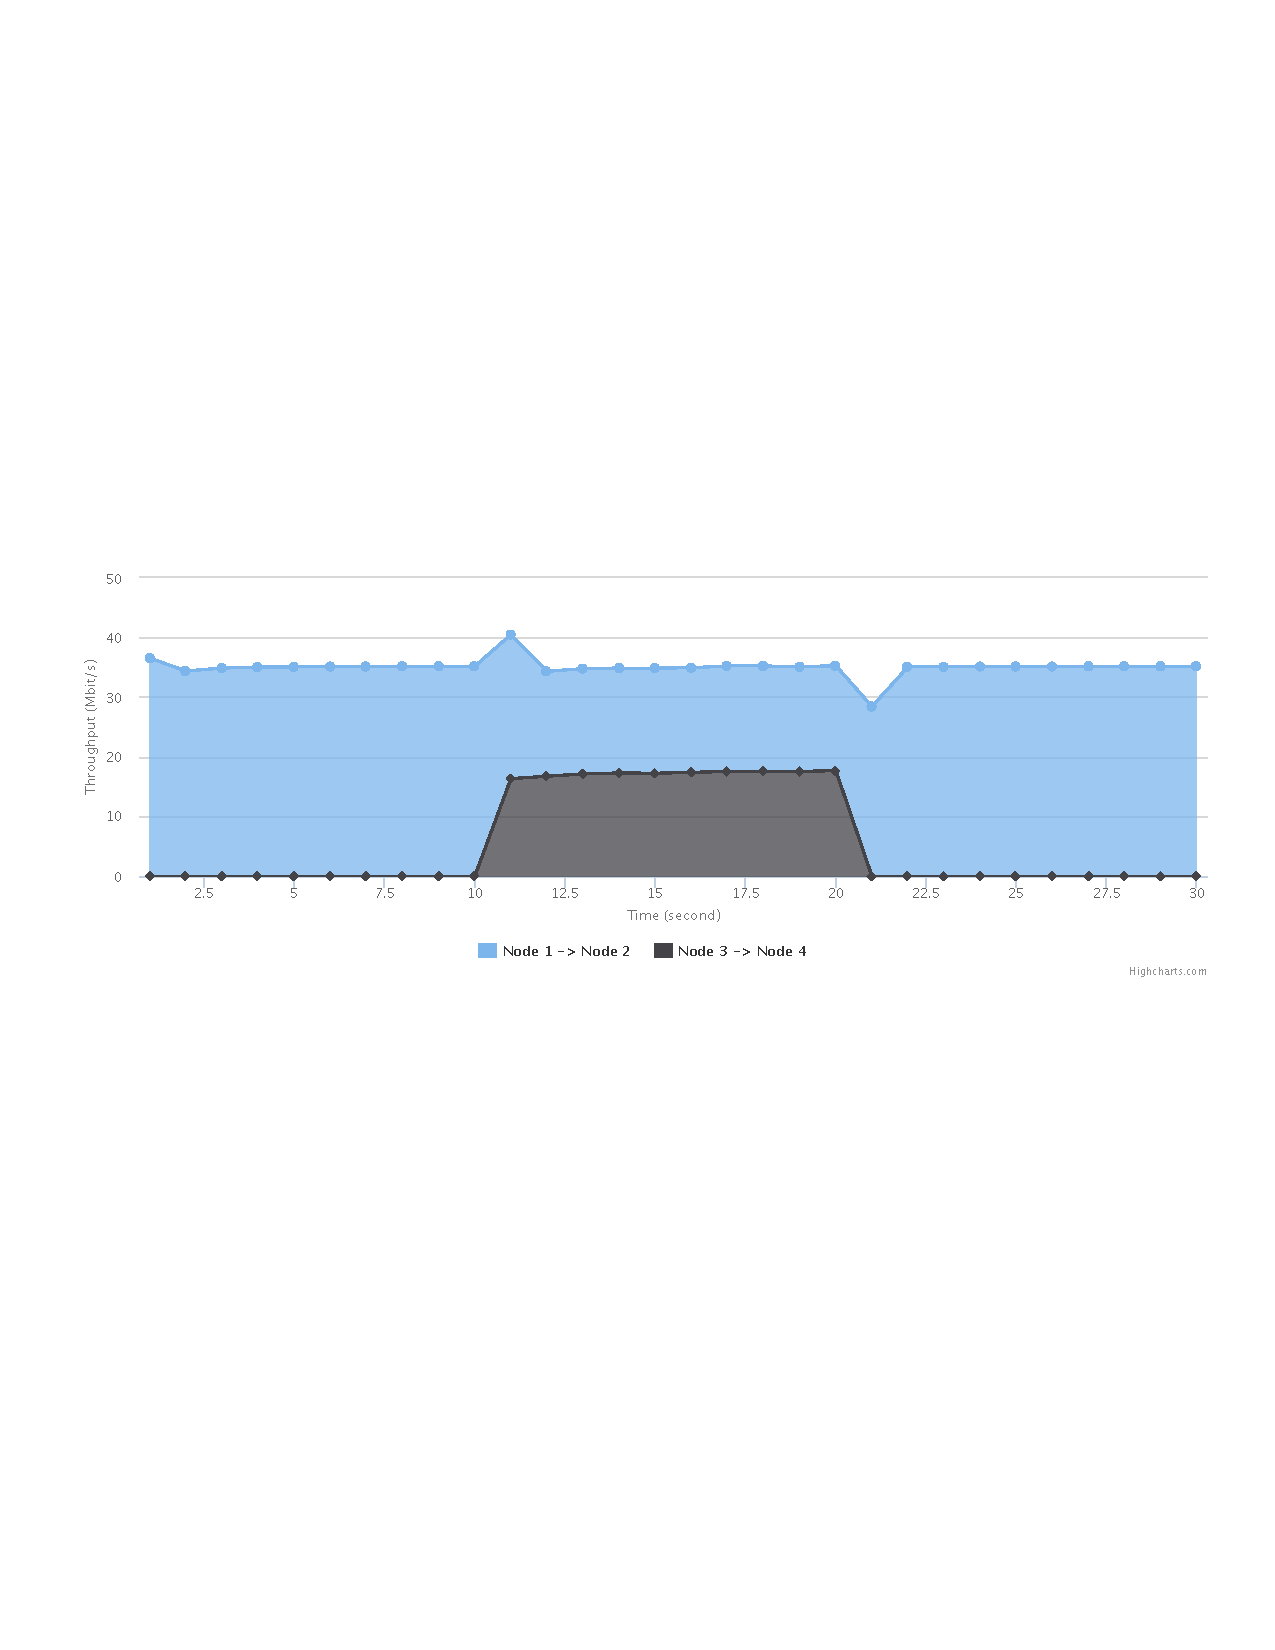
\includegraphics[width=1.1\textwidth]{figures/results/effectiveness_squirrel.pdf}}
      \caption{\label{fig:squirrel_preliminary_squirrel}Squirrel UDP Throughput}
    \end{subfigure}
    \caption{\label{fig:squirrel_preliminary}Squirrel CSMA/CA Model Testing: UDP Throughput in stacked area plot for Android v.s. Squirrel}
  \end{center}
\end{figure}

Figure~\ref{fig:squirrel_preliminary}\footnote{Plots in this dissertation are generated with Highchart JS (\url{https://http://www.highcharts.com/}) provided by Highsoft AS. Highchart JS is not free for commercial and Governmental use. The use of Highchart JS in this dissertation is under Creative Commons Attribution-NonCommercial 3.0 License.} shows a stacked area plot of the UDP throughput result from Android tablets and Squirrel. They both show that, in the first 10 seconds the first pair (node1 to node2) gets about 33 Mbps throughput. After the second pair (node3 to node4) starts at 10th second, the first pair's throughput drops to below 20 Mbps, while the second pair gets roughly the same level of throughput.

The general trends match very well between Android and Squirrel configuration and show the expected results. Squirrel is able to emulate interference based on positions of emulated nodes even though the traffic is between two different pairs that are completely independent. The difference is that, there seems to be more randomness in the Android test. This is likely due to networking channel condition variations due to external factors such as other devices beyond our control using 2.4 GHz, or even a microwave oven next door heating macaroni and cheese.

\subsection{Throughput Test}

Squirrel is a real-time emulator. Unlike in discrete event simulation where the model can take as long as it needs to calculate results, in real-time emulation, models need to make decisions as fast as events happen in real-world. In other words, raw throughput of Squirrel effectively bounds the scalability of emulation.

To find out this boundary, \texttt{iperf} is used to measure the throughput on Squirrel with PassThrough wireless model, which delivers all frames. The test was conducted on a single workstation with 6-core processor. All \texttt{squirrel-worker} nodes, as well as the \texttt{squirrel-master} run on the same workstation.

With a single pair of sender/receiver, UDP throughput achieves around 480 Mbps. This is mainly bounded by processor. As the number pairs increases to 2, more processor cores are able to work in parallel. As a result both pair get the same throughput, doubling the total throughput. However, when the number of pairs keep increasing, more parallel routines than the number of cores are requested, in which case the total throughput cannot increase linearly as number of pairs increases. Figure~\ref{fig:passthrough} is a stacked area plot showing UDP throughput with different pairs simultaneously transmitting. The total throughput tops at around 1200 Mbps, with each transmitting pair gets about 200 Mbps throughput.

\begin{figure}[h]
  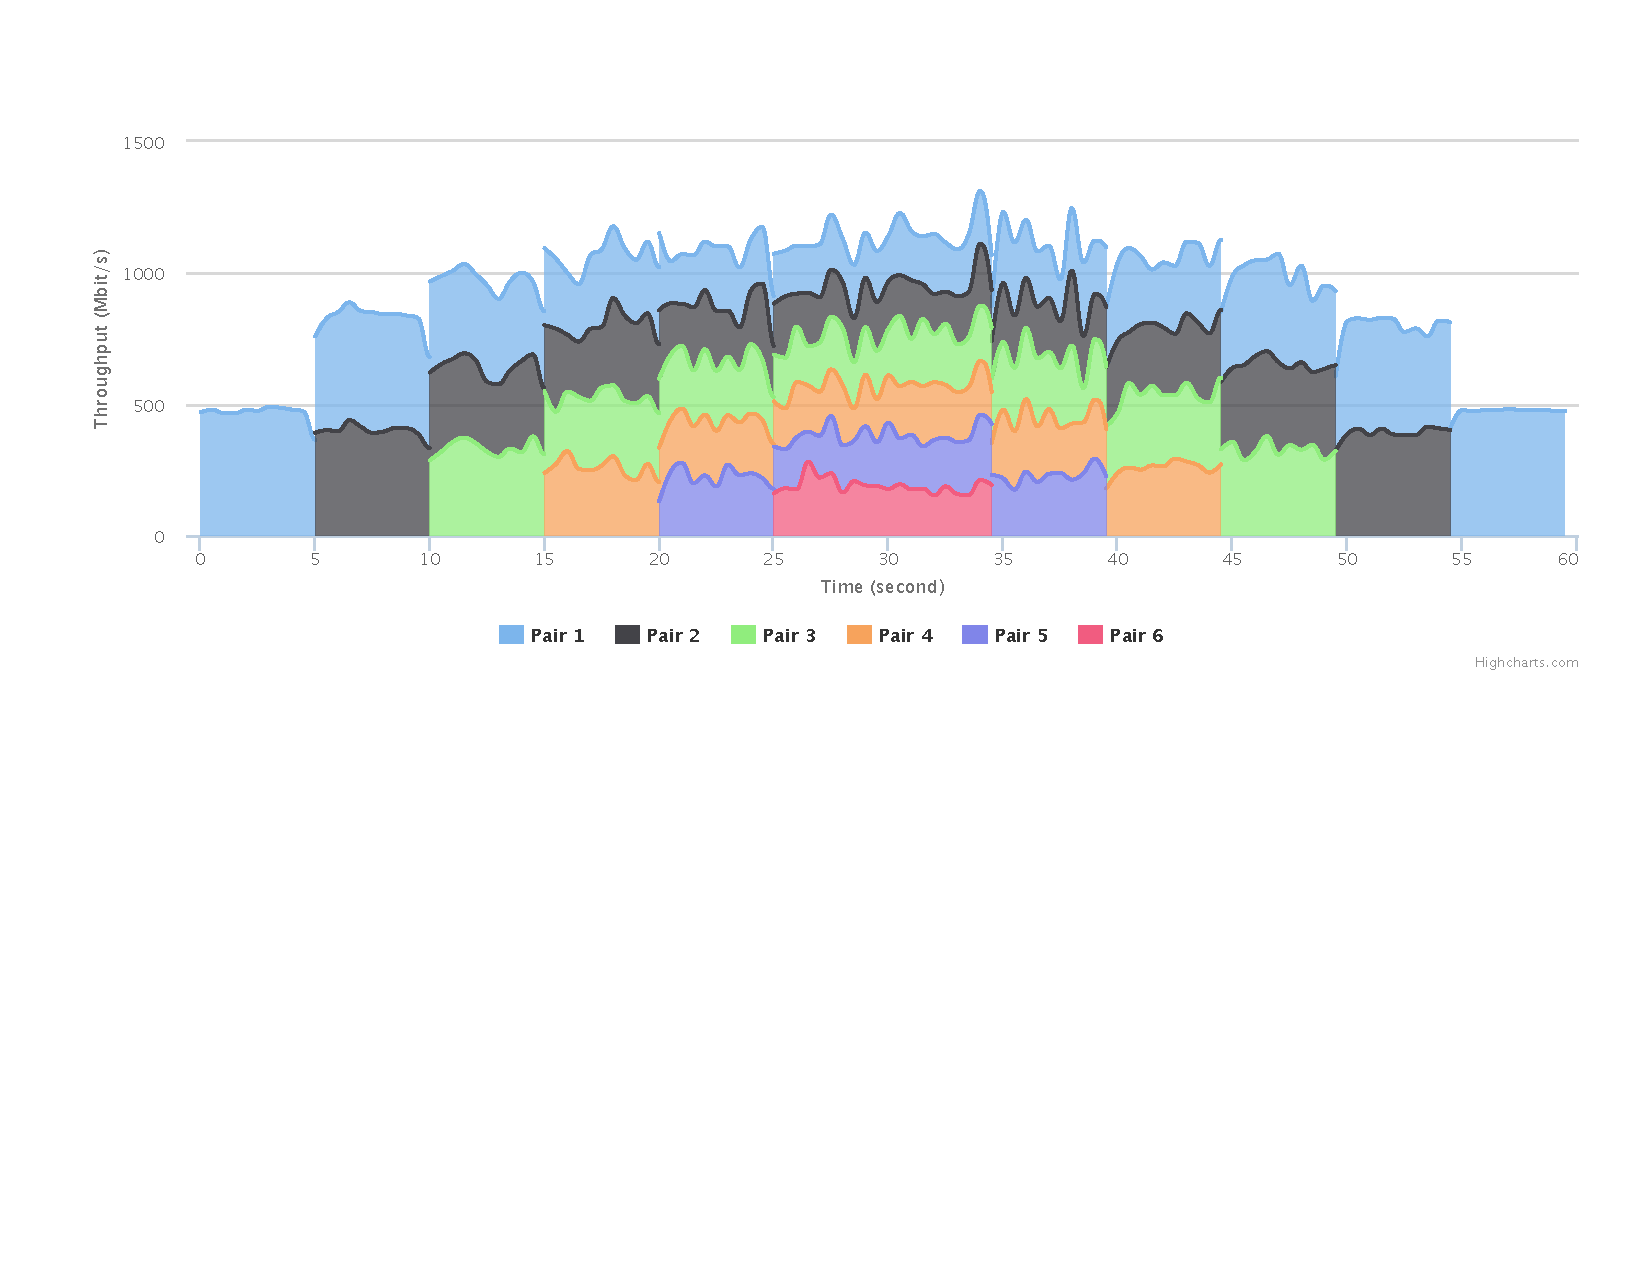
\includegraphics[width=\textwidth]{figures/results/passthrough.pdf}
  \caption{\label{fig:passthrough}Stacked Throughput using PassThrough Wireless Model}
\end{figure}

With more workstations handling \texttt{squirrel-worker} nodes and more number of cores on the workstations, the throughput can further increase. In other words, the throughput capability of Squirrel is mainly bounded by hardware resources. For the purposes in this study, a single workstation is able to provide enough throughput for the emulation.

\chapter{Inter-frame Compression Transmission Layer}

\section{Problem Statement}
\label{sec:problem_congestion}

In many cases for IEEE 802.11 communication, channel congestion is a key issue that affects performance, and needs to be relieved through various techniques. For DSRC channel congestion becomes a more important issue to consider, especially when the technology deployment scales to all vehicles on the road. There are several key factors that makes congestion problems in DSRC applications, especially safety application, more challenging:

\begin{enumerate}
  \item DSRC uses 10 MHz, for the purpose of supporting many parallel types of applications. However, the narrower channel width means the available bandwidth for the same channel is significantly reduced. Although applications can use different channels through channel switching, only the control channel is guaranteed to be accessed in every 100 millisecond window. Crucial safety application like vehicle platooning is less tolerable to channel unavailability, thus is likely to use control channel or a dedicated safety channel that has performance guarantees. As a result, 10 MHz channel width brings extra challenge to safety applications.
  \item As described in Section~\ref{sec:background_realworld_performance}, a previous study \cite{songDSRC2016} has shown that using two antennas on each vehicle and sending each message once on each antenna can significantly improve message delivery ratio. It is likely that the industry will adopt this approach more widely. This implies that twice as much of bandwidth would be required for the same application layer communication strategy, causing more pressure on the channel.
  \item The term ``Short Range" in DSRC is meant to convey that the communication range is shorter than cellular and WiMax services, but is still expected to reach a few hundred meters \cite{kenney2011}, which is much longer than the range of a typical WiFi deployment. Longer communication range means larger interference range. As a result DSRC causes congestion more easily than other IEEE 802.11 based protocols suites.
  \item Safety applications require real-time low latency data, thus is less tolerable to channel congestion. For example, in vehicle platooning, the back vehicle relies on periodical dynamics data from the front vehicle to maintain a close following distance. When channel is congested, several messages can be lost consecutively. In this case, the back vehicle has to make the worst assumption about the front vehicle, and apply strong braking in order to avoid collision.
\end{enumerate}

To show channel congestion can happen in busy road segments, some analysis is done to estimate bandwidth requirement in a typical platooning scenario on a busy segment of a highway environment. For analysis purposes, several assumptions are made and justified to assemble a reasonable heavy-use case:

\begin{enumerate}
  \item Average following distance: 20 meters. Study \cite{watts2015computational} has shown that fuel saving is significant when following distance is below 40 feet (about 13.3 meters). Volve \cite{volvo2015} has done real-world experiments with following distance of 7 meters. When there is traffic jam, following distance can be further reduced. Thus, assuming nearly full market penetration of Intelligent Transportation System (ITS\nomenclature{ITS}{Intelligent Transportation System}), 10 meters (or 0.33 seconds headway at 110 km/h) is a reasonable assumption for a moderately heavy-use case.
  \item Platooning message size: 150 bytes. SAE J2735 defines BasicSafetyMessage (BSM\nomenclature{BSM}{BasicSafetyMessage}), which includes various vehicle information helpful to vehicular safety applications. It has about 50 bytes of data that is requires portion and appears in every transmission. After the required portion, vendors can attach proprietary data structures. Since the required portion of BSM is not sufficient for platooning applications, the industry normally uses the custom portion extensively. 100 bytes is assumed for this part, which adds up to roughly 150 bytes for each platooning message.
  \item Total lanes: 10. In urban area, it is common for highways to have 5 lanes per direction at busy segments, especially near an interchange. In some cases, there are multiple highways in the same area, making congestion easier to happen. An example is an area\footnote{\url{https://www.google.com/maps/@33.6205067,-84.4576489,1936m/data=!3m1!1e3}} near Atlanta airport in US, where the Interstate 285 has 5 lanes per direction, with other roads or highways nearby. Thus, it is reasonable to use 10 lanes (for both directions) in analysis for heavy-use cases.
  \item Interference range: 400 meters. Interference range is larger than effective communication range. With DSRC ratios designed to reach several hundred meters, 400 meters' interference range is a reasonable assumption.
  \item MAC layer data rate: 6 Mbps. Study \cite{songDSRC2016} shows that even using alternate mode, the delivery ratio may drop significantly above 6 Mbps. Safety applications like platooning requires high reliability, so it is assumed that the 6 Mbps is selected all the time. This is not the most conservative choice. In some scenarios, 3 Mbps may be used to achieve higher reliability.
  \item Platooning message rate: 20 Hz. This assumes dual-antenna configuration and alternate mode. In other words, at 20 Hz, the effective message rate is 10 Hz, or one message every 100 milliseconds. 100 milliseconds results in about 3 meters in distance at a speed of 110 km/h. Depending on the braking system performance of the vehicle, this normally means tolerance of no more than 2 consecutive message losses before the control system has to conservatively apply a hard braking.
\end{enumerate}

Consider a target vehicle on a busy segment of a highway. With 400 meters' interference range, the vehicle is interfered by vehicles within 400 meters radius, which means an 800 meters long segment on the highway. Assuming full market penetration and full road utilization, linear vehicle density is $\frac{1 vehicle}{20 (meters*lane)}=0.05 vehicle/meter/lane$. With 10 lanes in total for both directions, there are $800 meters * 10 lanes * 0.05 vehicle/meter/lane = 400 vehicles$ within the interference range. At 20 Hz per vehicle, messages are being sent at $400 vehicles * 20 Hz/vehicle=8,000 Hz$ within the interference range. Multiplying this by the message size 150 bytes, the total demanded bandwidth can be calculated as $8,000 Hz * 150 bytes = 1.2 MB/second$, or 9.6 Mbps.

With variables defined as in Table~\ref{tab:bandwidth_equation_variable}, the calculation above can be represented in a streamlined equation as shown in Equation~\ref{eq:bandwidth}.

\begin{table}[h]
  \begin{center}
    \begin{tabular}{r l}
      \hline
      Variable & Definition \\ \hline
      $B$ & Demanded bandwidth within interference range \\
      $r$ & Interference range \\
      $l$ & Total number of lanes in both directions \\
      $d$ & Average following distance \\
      $s$ & Platooning message size \\
      $f$ & Frequency at which platooning messages are sent \\ \hline
    \end{tabular}
    \caption{\label{tab:bandwidth_equation_variable}Variable definition for Equation~\ref{eq:bandwidth}}
  \end{center}
\end{table}

\begin{equation}
  \begin{split}
    B & = \frac{2r}{d} * l * s * f = \frac{2 * 400m/lane}{20m/vehicle} * 10 lanes * 150 bytes * 20 Hz/vehicle \\
      & = 1.2 MB/second = 9.6 Mbps
  \end{split}
  \label{eq:bandwidth}
\end{equation}

9.6 Mbps is already greater than the MAC layer data rate 6 Mbps. Furthermore, due to the channel switching strategy defined in IEEE 1609.4 (see Section~\ref{sec:80211p}), only half of the channel time can be used. This reduces the available data rate to 3 Mbps. Other than this, there are MAC layer overheads, such as the contention window and various spacing in CSMA, management frames and control frames. These overheads further reduces the available bandwidth available for upper layers.

Even worse, the calculation above only considers the platooning message, which is an extended version of BSM. In addition to BSM, SAE J2735 also defines other message types usable in vehicular environment, including but not limited to: Common Safety Request, Emergency Vehicle Alert Message, Roadside Alert, Traveler Information, NMEA Corrections \cite{sae2016j2735,kenney2011}. These messages all increase bandwidth consumption, making the congestion worse.

In conclusion, the DSRC technology will have congestion problems when it is fully deployed. It is necessary to apply various techniques to reduce bandwidth consumption in DSRC applications in order to relieve channel congestion.

To reduce bandwidth consumption for platooning application and potential other vehicular applications, a transmission mechanism that uses interframe compression is designed in this study.

\section{Related Work}

In \cite{Wang2008howmuch}, the authors found that non-safety use of DSRC may have to be severely restricted during peak hours of traffic to insure that automotive safety is not compromised. This is consistent with the analysis in Section~\ref{sec:problem_congestion}.

Study \cite{huang2010adaptive} proposed an adaptive congestion control method that adapts communication rate and power based on the dynamics of a vehicular network and safety-driven tracking process. In \cite{fallah2010occupancy}, authors studied the relationship between channel occupancy, as a readily available feedback measure, controllable network parameters, and network performance, and proposed a closed loop congestion monitoring and control based on limited feedback from the network. Study \cite{Kenney2011linear} proposed a linear message rate control algorithm, which rather than using a binary control, takes advantage of full precision control inputs that are available on the wireless channel.

SAE J2945.1 \cite{sae2016j29451}, a standard that specifies the system requirements for vehicle-to-vehicle safety communications, includes a congestion control algorithm for BSMs. The algorithm inspects channel busy percentage and packet error rate, to make transmission decisions, including transmission schedule and radiate power.

These techniques in vehicular networks reduces bandwidth consumption by various congestion control methods. They reduce bandwidth consumption of vehicular applications significantly in congestion, but takes a different approach than this study:

\begin{itemize}
  \item First, the congestion control algorithms make decisions on when to limit message rate or transmitting powers. Consequently, message frequency or the amount of information transmitted are sacrificed, i.e., the networking service level degrades. In other words, to transmit the same amount of data, the required bandwidth is not reduced.
  \item Second, such congestion control algorithms are most effective when congestion already happens. They serve as a remedy for the consequences from congestion. However, the congestion control algorithms generally have little effect in prevention of congestion.
\end{itemize}

In this study, however, rather than trying to deal with the congestion when it happens, this study introduces a compression algorithm that helps postpone the point where congestion happens, by reducing bandwidth consumption without sacrificing the amount of information transmitted.

\section{Inspiration and Discussion}

Interframe compression is a fundamental idea of many video compression algorithms such as MPEG-2 \cite{le1991mpeg} and H.264 \cite{wiegand2003h264}. In video data, although entropy of each individual frame is relatively high, consecutive frames in a video are normally very similar, i.e., entropy of difference between consecutive frames is relatively low. Thus, encoding frames individually results is a waste of bandwidth. With interframe compression, video codecs encode complete frames (Intra-frames, or I-frames) only every once a while. Between these complete frames, only changing parts are encoded (Predictive-frames or P-frames, and Bidirectional-frames, or B-frame).

These frames are packed into Group of Pictures (GOP\nomenclature{GOP}{Group of Pictures}) structures. A typical GOP structure can be represented as \texttt{IBBPBBP$\ldots$PBBI}. Since B-frames and P-frames are much smaller than I-frames, the complete video stream uses much less bandwidth.

Messages in vehicular network can benefit from interframe compression as well. An important attribute of video streams that allows interframe compression is that consecutive frames are very similar, with only slight changes in parts. This is true for messages in vehicular environments as well. Many messages passed by DSRC applications only gradually change. Take platooning message as an example. Within a small portion of the road, e.g. 60 meters, or roughly 2 seconds at 110 km/h, many dynamic attributes of the vehicle, yaw rate, acceleration, brake system, steering, etc., have relatively stable values, as long as the vehicle is not doing a significant maneuver. Even when they change, they change gradually, which results in only a few flipped bits in binary form.

However, video compression algorithms cannot be directly applied to vehicular networks.

First, platooning messages, among many types of messages in vehicular environment, are temporal messages that are only meaningful within a period of time. As much as high delivery ratio matters, the message is of little use to the actual real-time applications if it is not delivered in time. As a result, the communication system should not attempt to delivery an old message by sacrificing latency of newer messages. In other words, retransmission should not happen in case of message losses. As a result, data stream from one vehicle to another should not be considered reliable, and key frames can be missing. Hence, a long dependency chain like \texttt{IBBPBBP$\ldots$PBBI} is not suitable for vehicular network.

Second, messages like platooning require lossless compression. While recent video compression techniques have improved prediction techniques and result in high quality video stream, they are not lossless and data through compression may still defer from original data.

Hence, to use interframe compression, a new algorithm needs to be designed to suit the needs of vehicular networks.

\section{Basic Design}

To make the transmission mechanism suitable for general purposes in vehicular environment rather than platooning specific, it is designed as a layer between Message Sublayer and WSMP layer in the DSRC stack as shown in Figure~\ref{fig:dsrc}. We call it Interframe Compression Transmission Layer (ICTL). In context of the DSRC protocol suite in Figure~\ref{fig:dsrc}, ICTL can be placed either between Safety Applications Sublayer and the Message Sublayer, or between Message Sublayer and WSMP.

In traditional DSRC, applications constructs a SAE J2735 message, and directly encapsulates it in a WSM and send through IEEE 802.11p using WSMP. With ICTL, the message is either sent as it is, or converted to a smaller byte stream containing changes from a previous complete message before being sent out. ICTL takes care of compression and decompression, and applications see the same message identical to the original.

To support this, two types of frames are introduced:

\begin{itemize}
  \item Key Frame (KF). A KF is like an I-frame in video compression. It contains complete message being sent. It does not require any extra information to decode a KF.
  \item Differential Frame (DF). A DF only carries difference from a previously sent KF. Decoding original message from a DF requires the KF that it refers to as well.
\end{itemize}

\subsection{Header and Layout}

To separate DF from KF, identify each message, and carry extra information regarding to codings, ICTL uses a 4-byte header. Table~\ref{tab:ictl_layout} shows the layout of an ICTL packet. Zooming out to a bigger picture, a typical message with all headers has a layout shown in Table~\ref{tab:ictl_layout_wsm}.

\begin{table}[h]
  \begin{center}
    \begin{tabular}{|c|c|c|c|c|}
      \hline
      Reserved & Frame Type & Compression Options & Frame ID & Payload \\\hline
      4 bits   &  4 bits    & 8 bits              & 16 bits  & variable length \\\hline
    \end{tabular}
    \caption{\label{tab:ictl_layout}ICTL Packet Layout}
  \end{center}
\end{table}
\begin{table}[h]
  \begin{center}
    \begin{tabular}{|c|c|c|c|}
      \hline
      MAC Header (IEEE 802.11) & WSM Header & ICTL Header & Payload \\\hline
      34 bytes            & 5-20 bytes & 4 bytes     &  variable length \\\hline
    \end{tabular}
    \caption{\label{tab:ictl_layout_wsm}ICTL Packet Layout With WSM Header}
  \end{center}
\end{table}

The Reserved field is in case of a newer version of ICTL. For now it should always be set to \texttt{0b0000}. In the future, this field can be used as a version field. Frame Type indicates whether the packet contains a KF (\texttt{0b0001}) or a DF (\texttt{0b0010}). Compression options carries information about compression algorithms applied to the payload (see Section~\ref{sec:ictl_process}). Frame ID is an increasing unsigned integer that wraps at boundaries. It is used to identify frames sent from the same source. For a KF, it is the ID of the actual message. For a DF, it is the ID of the KF that it refers to. Payload is the actual complete message (KF) or differential message (DF). Since WSM header already has a field for payload length, and ICTL header has a fixed width of 4 bytes, the length of ICTL payload can be easily inferred, thus does not require an extra length field.

\subsection{Differential Encoding}
\label{sec:ictl_diff}

Compressing vehicular messages needs to be lossless. As a result, video compression techniques such as prediction cannot be used. Instead, a simpler approach using Exclusive Or (XOR\nomenclature{XOR}{Exclusive Or}) is proposed to encode differential messages in a DF.

Given a previously transmitted KF, whose payload is
\begin{equation}
  p^0={b^0_0,b^0_1,b^0_2,b^0_3,b^0_4,b^0_5,\ldots,b^0_{n-2},b^0_{n-1}}
\end{equation}
where $b^0_i$ represents one bit (zero based index) of the payload $p^0$, and a new message
\begin{equation}
  p^1={b^1_0,b^1_1,b^1_2,b^1_3,b^1_4,b^1_5,\ldots,b^1_{n-2},b^1_{n-1}}
\end{equation}
where $b^1_i$ represents one bit (zero based index) of the payload $p^1$, then the payload of DF, or in other words, the differential message $d^{0,1}$ between $p^0$ and $p^1$, can be produced as
\begin{equation}
  d^{0,1}={b^0_0\oplus b^1_0,b^0_1\oplus b^1_1,b^0_2\oplus b^1_2,b^0_3\oplus b^1_3,b^0_4\oplus b^1_4,b^0_5\oplus b^1_5,\ldots,b^0_{n-2}\oplus b^1_{n-2},b^0_{n-1}\oplus b^1_{n-1}}
\end{equation}
where $\oplus $ is XOR operator\footnote{When implementing in a programming language, this can be done efficiently by using bitwise XOR operator (normally written as $\hat{\ }$), and computed one byte, or even one word (32 bits or 64 bits) at a time.}.

Since the messages that are sent within a short time window have very similar content, the majority bits in the differential message should be zero. Such message has low entropy, and can be efficiently compressed using a general purpose compression algorithm.

\subsection{Encoding and Decoding Process}
\label{sec:ictl_process}

ICTL is per application rather than per link. Since WSMP already handles multiplexing through PSID, ICTL does not further multiplex messages into multiple streams. In other words, one ICTL encoder/decoder should be allocated for each PSID.

When ICTL receives a request to transmit message from upper layer for a given PSID, it first determines whether the message should be transmitted using KF or DF. This depends on either a predefined parameter that describes how many DFs can be sent between two adjacent KFs, or an internal model to make the decision.

For KF, the message is compressed, and prepended with an ICTL header. The header indicates that it is a KF, and provides the increasing unsigned integer to identify the message. For DF, the differential message is first calculated using process described in Section~\ref{sec:ictl_diff}, then compressed and prepended with ICTL header. The header indicates that it is a DF, and references the ID of the KF that the DF is produced from. Normally, the referenced KF is the most recently sent KF, but can be older ones as well depending the networking condition when the KF was sent. If the network condition was bad when the most recently sent KF was transmitted, it might not have been successfully received by many vehicles nearby. In this case, ICTL can choose a previously sent KF to base on. In this study, however, for simplicity, ICTL always choose the most recently sent KF as reference frame.

Following is a pseudo-code listing for encoding KFs and DFs using Go-like syntax:

\begin{singlespace}
  \lstinputlisting{ictlEncoding.go.lst}
\end{singlespace}

Decoding is basically the reverse operation of encoding. Since the sender may choose to send a differential message based on an older message, a list of recently received KF needs to be maintained. Following is a pseudo-code listing for decoding KFs and DFs using Go-like syntax:

\begin{singlespace}
  \lstinputlisting{ictlDecoding.go.lst}
\end{singlespace}

The implementations of \texttt{shouldDF()} is particularly tricky, and requires to be guided by tests in order to achieve good performance. The following sections of this chapter explains this process, in which an adaptive ICTL algorithm (Section~\ref{sec:adaptive_ictl}) is designed.

For analysis and experimental purposes, the concept of ICTL Cycle, and Cycle Length (CL\nomenclature{CL}{Cycle Length}) is introduced here:
\begin{itemize}
  \item ICTL Cycle is defined as a sequence of ICTL frames, starting with a KF, followed by a number of DFs, given that the last DF, i.e., the end of cycle, is either the last frame of transmission, or followed immediately by a KF, which marks the start of next cycle. In the case of this study where ICTL always pick the most recently transmitted KF as reference frame for DFs, an ICTL Cycle can also be defined as a sequence messages including exactly one KF, and all DFs that use this KF as reference frame;
  \item CL is defined as the number of messages included in an ICTL Cycle. For example, for an ICTL strategy that always sends 3 DFs after each KF before sending a new KF, the CL is always 4. CL can be a predefined fixed value, in which case it is a configurable parameter, or dynamically changing according to an internal model in ICTL implementation, in which case CL is merely an observed value driven by the ICTL implementation.
\end{itemize}

\section{Implementation and Experimental Setup}

\subsection{Implementation}

For the same reasons explained in Section~\ref{sec:squirrel_implementation}, Go programming is chosen to implement ICTL. Similarly, it uses a buffer pool for memory management. ICTL is implemented as a library package that encapsulates details of encoding and decoding behind a simple interface \texttt{ictl.Endpoint}, which represents an ICTL endpoint for encodings and decodings. An object of \texttt{ictl.Endpoint} can be created using a configuration object that specifies the behaviors of ICTL algorithm, and the endpoint has methods for encoding and decoding messages. Each of such methods accepts a \texttt{context} parameter, which is used to differentiate different streams of data. In case of DSRC, a combination of MAC address and PSID is a good choice of \texttt{context}. The endpoint allocates one encoder/decoder for each context, and maintains the separation between different data streams.

\subsection{Trace File Playback}
\label{sec:truck_playback}

Squirrel was designed to facilitate running real-world code. Everything above MAC layer assumes a real wireless device, and process real network frames. The idea here is to develop research projects that can be not only reproducible, but also more directly beneficial to real-world applications. With the same spirit, we acquired real-world platooning data traces, and use them to study the ICTL algorithm, and make performance improvements. To utilize such trace files, a software component is written, called \texttt{truck-playback}, to replay events from one vehicle.

The trace files were logged by platooning applications running on two heavy vehicles, while the trucks were being tested with platooning on a closed test track. The trace files include many events, such GPS location, DSRC messages transmission and reception, various events from vehicle's CAN bus, radar measurements, etc.. For the purpose of studying ICTL, two events are relevant:

\begin{itemize}
  \item GPS location events, which are needed to update emulated locations of the truck in Squirrel;
  \item DSRC transmission events, which indicate when to send a DSRC message, and what particular data should each DSRC message carry.
\end{itemize}

\texttt{truck-playback} reads the two types of events from a logged trace file, and replays these events in emulation. The GPS location events are converted to RPC requests, and sent through the RPC Updated Mobility Manager's service (see Section~\ref{sec:rpc_mobility_manager}), to update current emulated position of the node. The DSRC events drives the \texttt{truck-playback} to send WSMs over DSRC at predefined time points, using traditional method, or encoded with ICTL. The content of a WSM is determined by the event content, which includes values of each data field. Sending exactly the same information as trace files is important, because the content of messages, and how fast the content changes, affect how well ICTL compresses the messages.

Each event from the trace file is tagged with a timestamp. \texttt{truck-playback} synchronizes the timeline so that a time point from wall-clock during emulation is aligned with a time point from trace file's time while tests were conducted in real-world. In other words, a fixed offset is set between the playback's timeline and the trace file's timeline. When \texttt{truck-playback} replays an event, it first calculates a deadline based on the timeline offset. In most cases, the deadline is after current wall-clock time. A difference is calculated between the two, and \texttt{truck-playback} waits for such time duration by calling \texttt{sleep()} before actually replaying the event. This ensures that events happen at exactly same relative times. For example, DSRC messages are sent at same frequencies as the trace file dictates. When many nodes are emulated on the same computer, occasionally, the deadline may have already passed at time it's calculated. In this case, this particularly event is sent immediately (without calling \texttt{sleep()}, but not able to meet the deadline when replayed. If too many events cannot meet deadline, the results would not be authentic. As a result, \texttt{truck-playback} logs the such incidents to be examined afterwards.

The \texttt{truck-playback} uses a WSMP implementation written in Go, which uses system call interfaces to pass messages into, or read messages from Logical Link Control (LLC\nomenclature{LLC}{Logical Link Control}) layer in the kernel. In Squirrel emulation, LLC is handled by \texttt{squirrel-worker} through \texttt{tap0} interface, as demonstrated in Figure~\ref{fig:squirrel_arch}. Conceptually, \texttt{truck-playback} works as a DSRC application as shown in Figure~\ref{fig:playback_arch}.

\begin{figure}[h]
  \begin{center}
    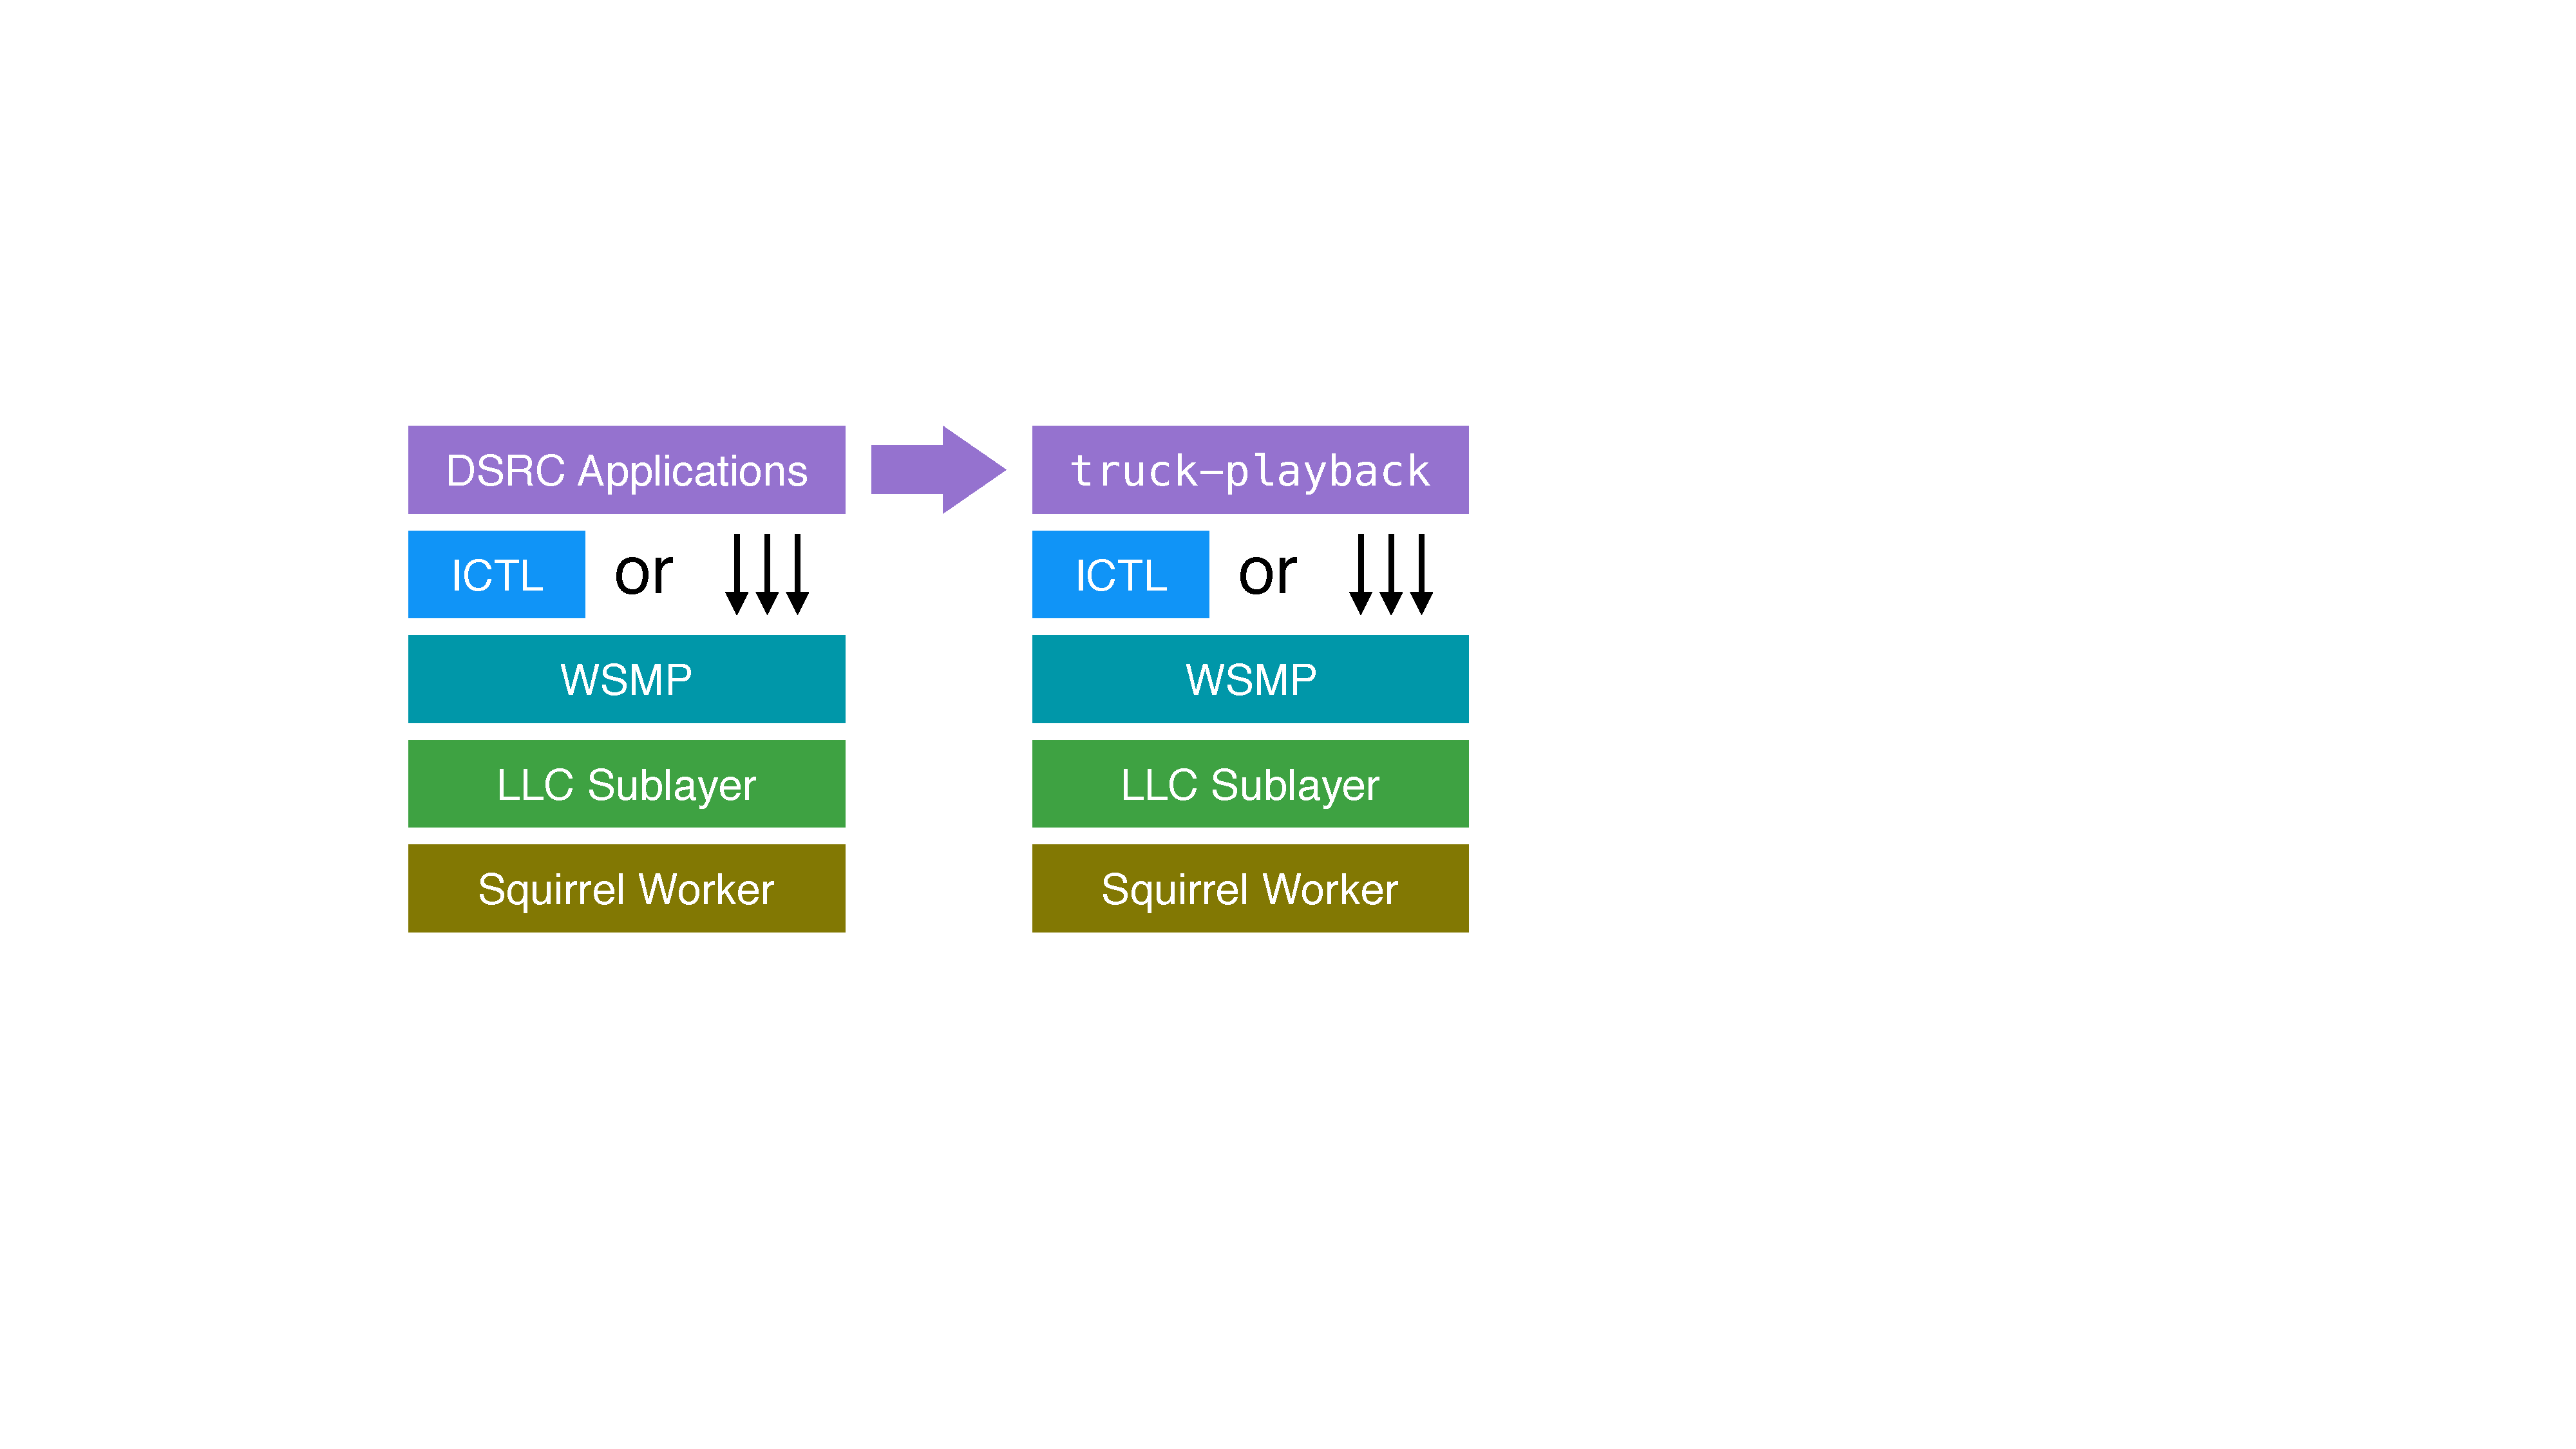
\includegraphics[width=.6\textwidth]{figures/playback_arch.pdf}
    \caption{\label{fig:playback_arch}\texttt{truck-playback} as DSRC Application}
  \end{center}
\end{figure}

When \texttt{truck-playback} replays a DSRC transmission event, it logs the replay, including a timestamp, the GPS position of the node when the message is sent, a message counter, and frame size. Similarly, when it receives a message from WSMP, it logs the reception as well, including a timestamp, a message counter, source MAC address, and frame size. With these information, we can study bandwidth and delivery ratio of ICTL, under different parameter scenarios.

\subsection{Deployment}

Squirrel can be deployed on a cluster, where one node runs \texttt{squirrel-master}, and \texttt{squirrel-worker} nodes run on other nodes. In this study, however, the cluster only consists of one physical workstation. The workstation has one Intel(R) Xeon(R) CPU W3680 with 6 cores. The CPU does not have hyper-threading technology, so at maximum 6 threads (as opposed to 12 threads had it support hyper-threading technology) can run simultaneously on the CPU at any time.

For its lightweight and scalability, OSLV is chosen to provide proper isolation for different emulated nodes. Specifically, each \texttt{squirrel-worker} node runs in an application container \cite{menage2007adding}. With different kernel namespaces, one isolated complete networking stack is allocated for each \texttt{squirrel-worker} node. There are several open source softwares providing Linux application container runtime, namely Docker, LXC, and Rkt. Each of them provides a set of tools to build container image, and to run and configure application containers. In this study, Rkt \cite{rkt} is used. The operating system on the workstation is CoreOS \cite{coreos}, a modern Linux distribution designed specifically for running application containers.

Since all components are written in Go, they are statically linked into independent executable binaries, which makes packaging Rkt images very straightforward. The \texttt{squirrel-master} image only contains the \texttt{squirrel-master} binary. The \texttt{squirrel-worker} node image contains the \texttt{squirrel-worker} binary, \texttt{truck-playback} binary. For convenience of debugging, and some common tools such as \texttt{tcpdump} and a command-line shell, are also included. Since application containers provide filesystem isolation as well, proper filesystem mount points are configured for \texttt{squirrel-worker} nodes to provide input data trace files as well as to collect logs from \texttt{truck-playback}.

CoreOS uses \texttt{systemd} as its init system. To manage massive \texttt{squirrel-worker} nodes for experiments, \texttt{systemd} unit files are written to use \texttt{systemd} to automatically spawn Rkt containers, attach directories to mount points, and provide initial parameter settings. A wrapper unit file is also written to automatically schedule series of tests consisting of different number of nodes and configurations.

\subsection{Triggering Congestion}
\label{sec:trigger_congestion}

A major goal that ICTL tries to achieve by reducing bandwidth consumption is to improve delivery ratio when network utilization is high. As a result, to study and improve ICTL, it is necessary to create congestion in the emulation environment. Section~\ref{sec:problem_congestion} uses 400 vehicles in the analysis. However, on a single workstation, it is hard to emulate 400 nodes in real time. The data trace files we acquired use 50 Hz DSRC message rate, which is higher than 20 Hz in the analysis, which already makes it easier to trigger congestion. In addition, several methods are used to help trigger congestion with less than 15 emulated nodes.

\begin{enumerate}
  \item 3 Mbps (instead of 6 Mbps) is used as the MAC layer data rate setting in Squirrel's CSMA/CA model.
  \item Each message is replicated 12 times, in 12 separate WSMs, before being encapsulated and sent as a LLC layer frame. This increases frame size, in case of original data trace, from 117 bytes to 1250 bytes.
\end{enumerate}

Part of replicated messages in second method can also be seen as adding other DSRC messages into the frame. An important example is re-broadcast messages that are required to deliver message to vehicles outside transmission range.


\subsection{First Glance}

A simple test is run in the emulation platform to demonstrated the effectiveness of ICTL. In Figure~\ref{fig:first_glance}, three strategies are compared. ``Raw" series shows the demanded bandwidth of the original data trace; ``Raw Compressed" shows the demanded bandwidth of the data trace compressed with a traditional compression algorithm \footnote{\texttt{flate} is used here. Please refer to Section~\ref{sec:payload_compression} for more information on choice among different compression algorithms.}; and ``ICTL CL=3" shows the demanded bandwidth of the data trace compressed using ICTL, with fixed CL 3.

\begin{figure}[h]
  \makebox[\textwidth][c]{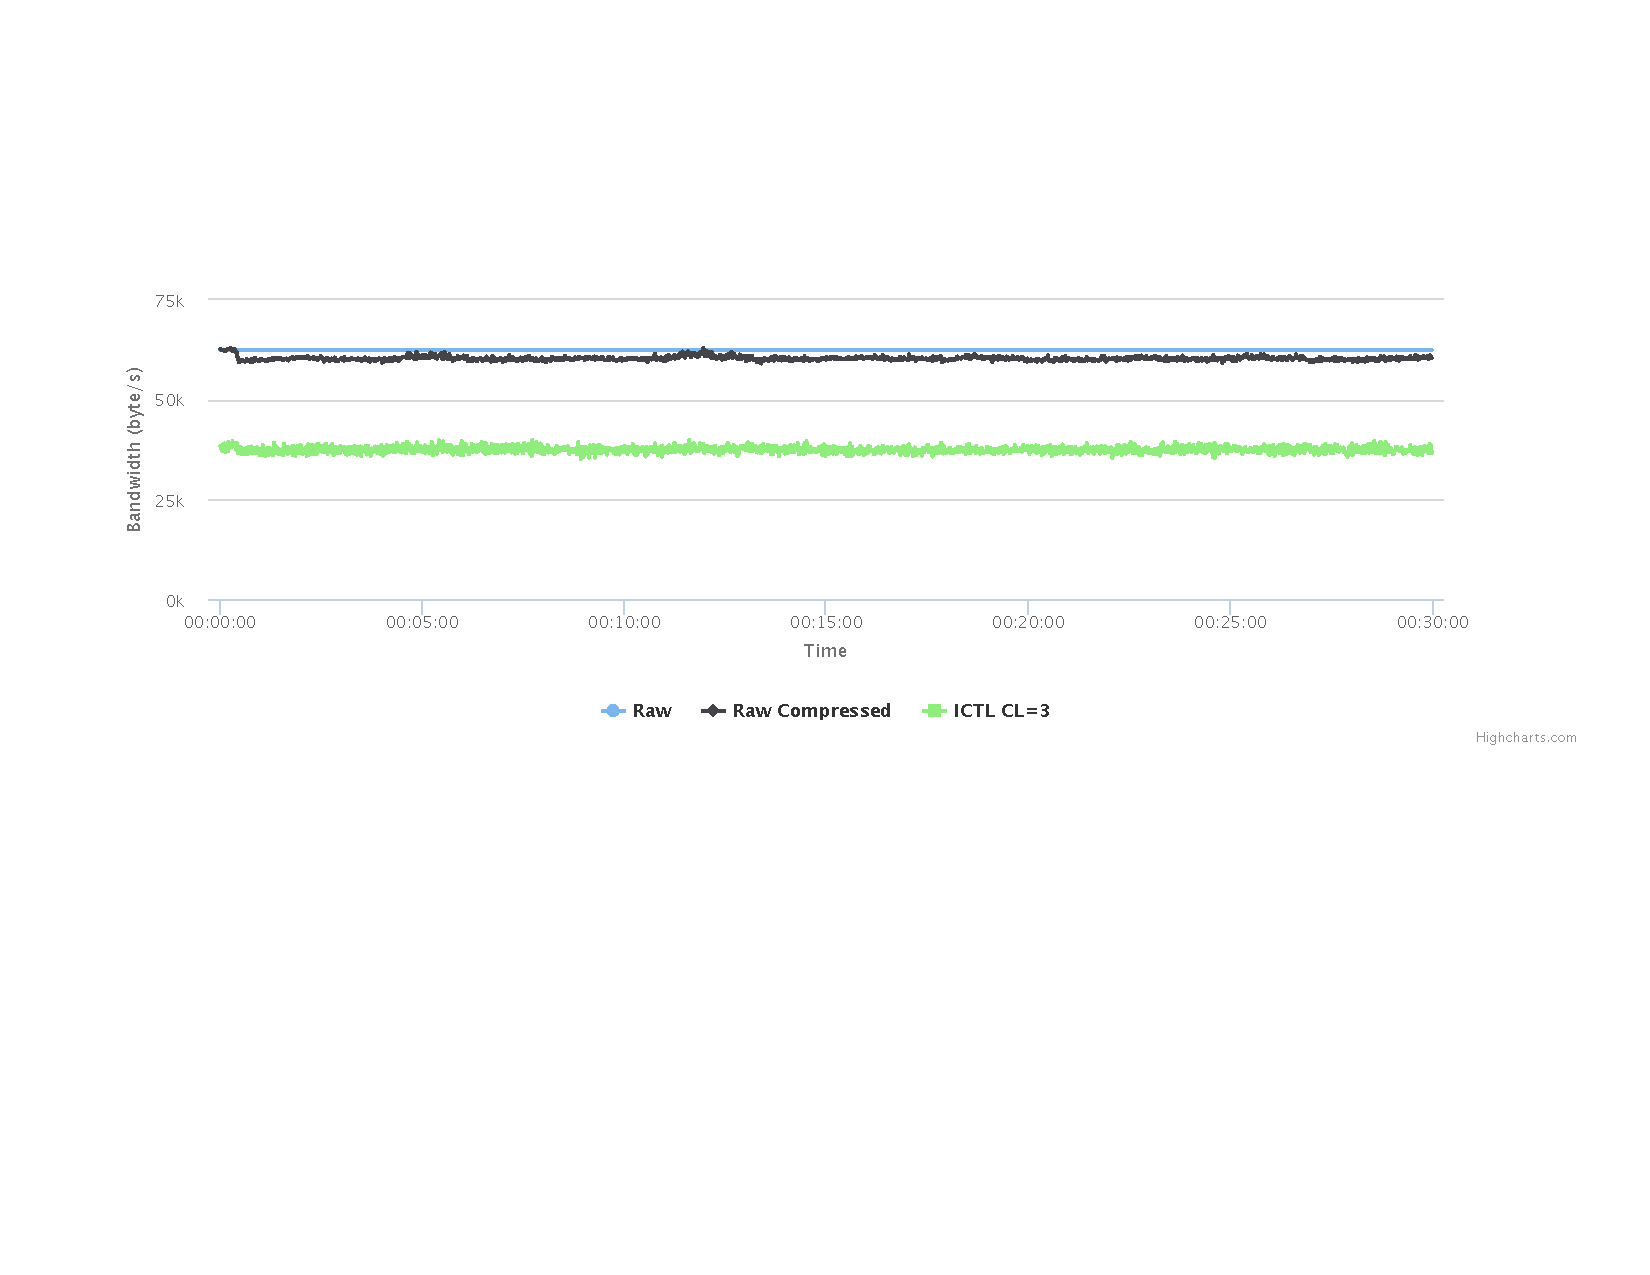
\includegraphics[width=1.1\textwidth]{figures/results/first_glance.pdf}}
  \caption{\label{fig:first_glance}Bandwidth test: Original, Traditional Compression, and ICTL }
\end{figure}

In this test, the original data trace uses a constant bandwidth of 62.5 KB/s. Using traditional compression method directly over original data trace uses $\ge$ 59 KB/s. With ICTL, the demanded bandwidth is always below 40 KB/s, yielding more than 30\% bandwidth savings.

The test demonstrates the effectiveness of the basic idea of ICTL. Following sections in this chapters studies behavior and performance attributes of ICTL, and describe ways to optimize the algorithm for bandwidth and delivery ratio.


\section{Performance Studies}

\subsection{Cycle Length and Application Delivery Ratio}
\label{sec:cl_adr}

Delivery ratio is one of the ultimate metrics that researchers are constantly trying to optimize for. In this case, two kinds of delivery ratio are involved:

\begin{itemize}
  \item Application Delivery Ratio (ADR\nomenclature{ADR}{Application Delivery Ratio}) is the delivery ratio observed in application layer. Lost frames or errors in any of the lower layers can affect this metric. This is the metric that we are trying to optimize for.
  \item Network Delivery Ratio (NDR\nomenclature{NDR}{Network Delivery Ratio}) is the delivery ratio observed in the layer immediately below ICTL. Events such MAC layer frame loss directly affect this metric.
\end{itemize}

In ICTL, each DF carries differential information from a previously transmitted KF. In other words, decoding a DF depends on the success of a KF transmission. As a result, losing a KF can be critical, since it implies the loss of all frames within the cycle starting with the lost KF. This makes the relationship between ADR, CL and NDR more complicated. On one hand, longer CL means more application frame loss whenever a key frame is lost; on the other hand, longer CL means that there are less KFs in the same transmission, thus losing KFs is less likely to happen given the same NDR.

Some mathematical analysis is done to further study this problem. Table~\ref{tab:cl_var} shows variables used in the analysis, along with their meanings.

\begin{table}
  \begin{center}
    \begin{tabular}{r l}
      \hline
      Variable & Definition \\ \hline
      $N$      & The number of messages needed to be transmitted \\
      $n_a$    & The number messages delivered at application layer during entire transmission \\
      $n_c$ & The number of messages delivered at application layer within one ICTL Cycle \\ 
      $m$      & CL \\
      $p_n$    & The probability that an ICTL frame is delivered, i.e., not lost in lower layers \\
      $NDR$    & NDR \\
      $ADR$    & ADR \\
      \hline
    \end{tabular}
    \caption{\label{tab:cl_var}Variable Definition for Analysis in Section~\ref{sec:cl_adr}}
  \end{center}
\end{table}

Assume that $N$ is sufficiently large, then $p_n$ is equal to $NDR$, and $ADR$ can be calculated as $\frac{n_a}{N}$. Starting from each ICTL Cycle, the expected number of messages delivered at application layer within on ICTL Cycle, $E[n_c]$, can be calculated by dividing into two cases:
\begin{enumerate}
  \item When the KF is lost, the entire ICTL Cycle is lost, i.e., 0 is delivered. The probability of this happening is $1-p_n$;
  \item When the KF is delivered, each message in the rest of the ICTL Cycle is delivered at probability of $p_n$, so the expected number of delivery of the cycle in this case is $1+(m-1)*p_n$ The probability of this happening is $p_n$.
\end{enumerate}

So $E[n_c]$ can be calculated using Equation~\ref{eq:expected_nc}:

\begin{equation}
  \begin{split}
    E[n_c] & = (1-p_n) * 0 + p_n * [1 + (m - 1) * p_n] \\
           & = p_n^2 * m - p_n^2 + p_n
  \end{split}
  \label{eq:expected_nc}
\end{equation}

With $N$ frames in total, and CL being fixed at $m$, there are $\frac{N}{m}$ ICTL cycles in total. So ADR can be calculated using Equation~\ref{eq:adr0}:

\begin{equation}
  ADR = \frac{E[n_a]}{N} = \frac{\frac{N}{m}E[n_c]}{N} = \frac{E[n_c]}{m}
  \label{eq:adr0}
\end{equation}

Combining Equation~\ref{eq:expected_nc} and \ref{eq:adr0},

\begin{equation}
  \begin{split}
    ADR = \frac{E[n_c]}{m} & = \frac{p_n^2*m-p_n^2+p_n}{m} \\
                           & = p_n^2 + \frac{p_n-p_n^2}{m}
  \end{split}
  \label{eq:adr}
\end{equation}

\begin{figure}[h]
  \begin{center}
    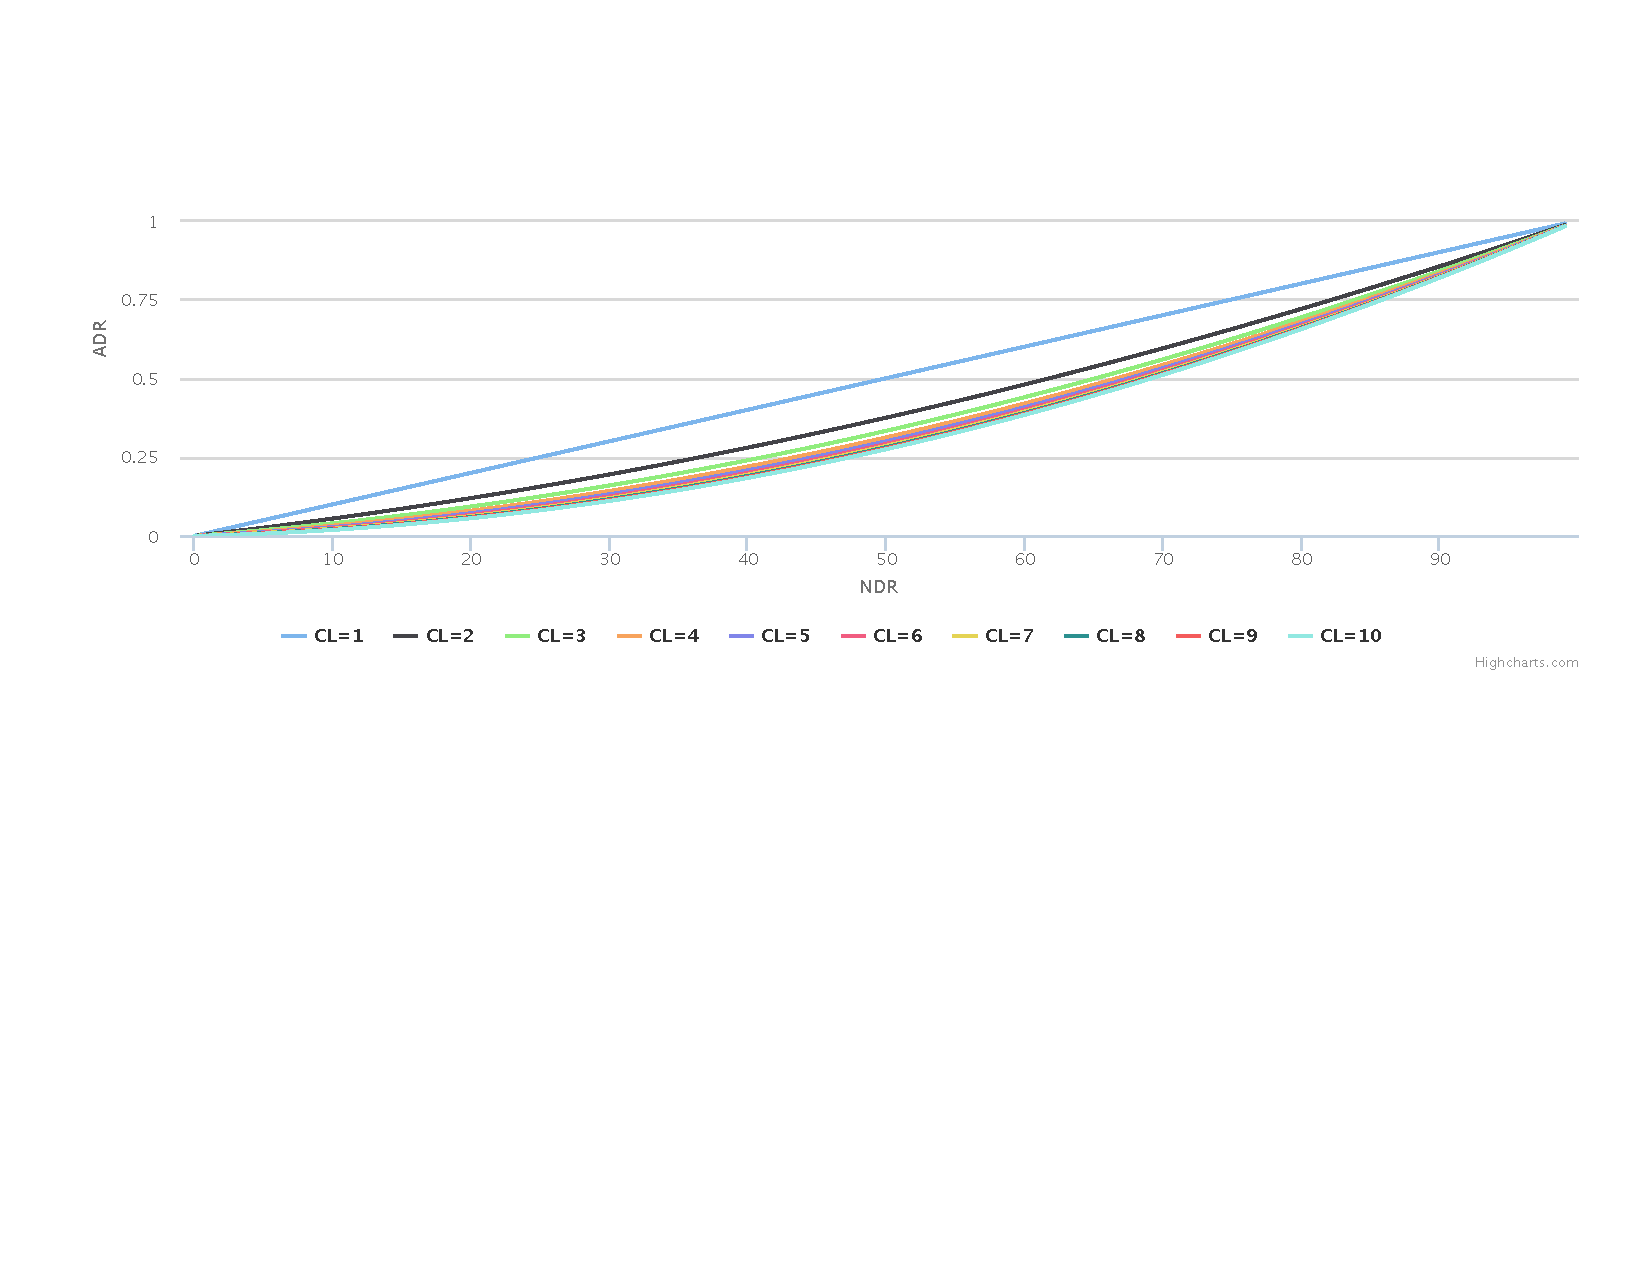
\includegraphics[width=\textwidth]{figures/adr.pdf}
    \caption{\label{fig:adr}ADR as function of NDR for different CL}
  \end{center}
\end{figure}

Equation~\ref{eq:adr} shows the relationship between ADR, NDR, and CL. This is illustrated in Figure~\ref{fig:adr}, which shows ADR as function of NDR for different CL values. Although higher CL values brings down lower ADR overall, ADR is not as sensitive to CL changes as to NDR changes. In other words, ADR is more affected by NDR.

Bandwidth consumption affects NDR in a major way, in the sense that lower bandwidth consumption means less congestion, which results in higher NDR. As a result, for the purpose of increasing ADR, it is reasonable for ICTL to simply optimize for low bandwidth.

\subsection{Location and Bandwidth}

ICTL compresses difference between frames, so it uses less bandwidth when frames are more similar, and uses more bandwidth when frames change more drastically. When a vehicle goes through a curve, vehicle's status, such as yaw rate, may change more than on a straight line. Intuitively, one may think ICTL should result in more bandwidth consumption at curves compared to on straight lines. To find out whether this is true, Figure~\ref{fig:3d}, a 3D version of Figure~\ref{fig:first_glance}, is generated, to show bandwidth consumption at different locations.

\begin{figure}[h]
  \makebox[\textwidth][c]{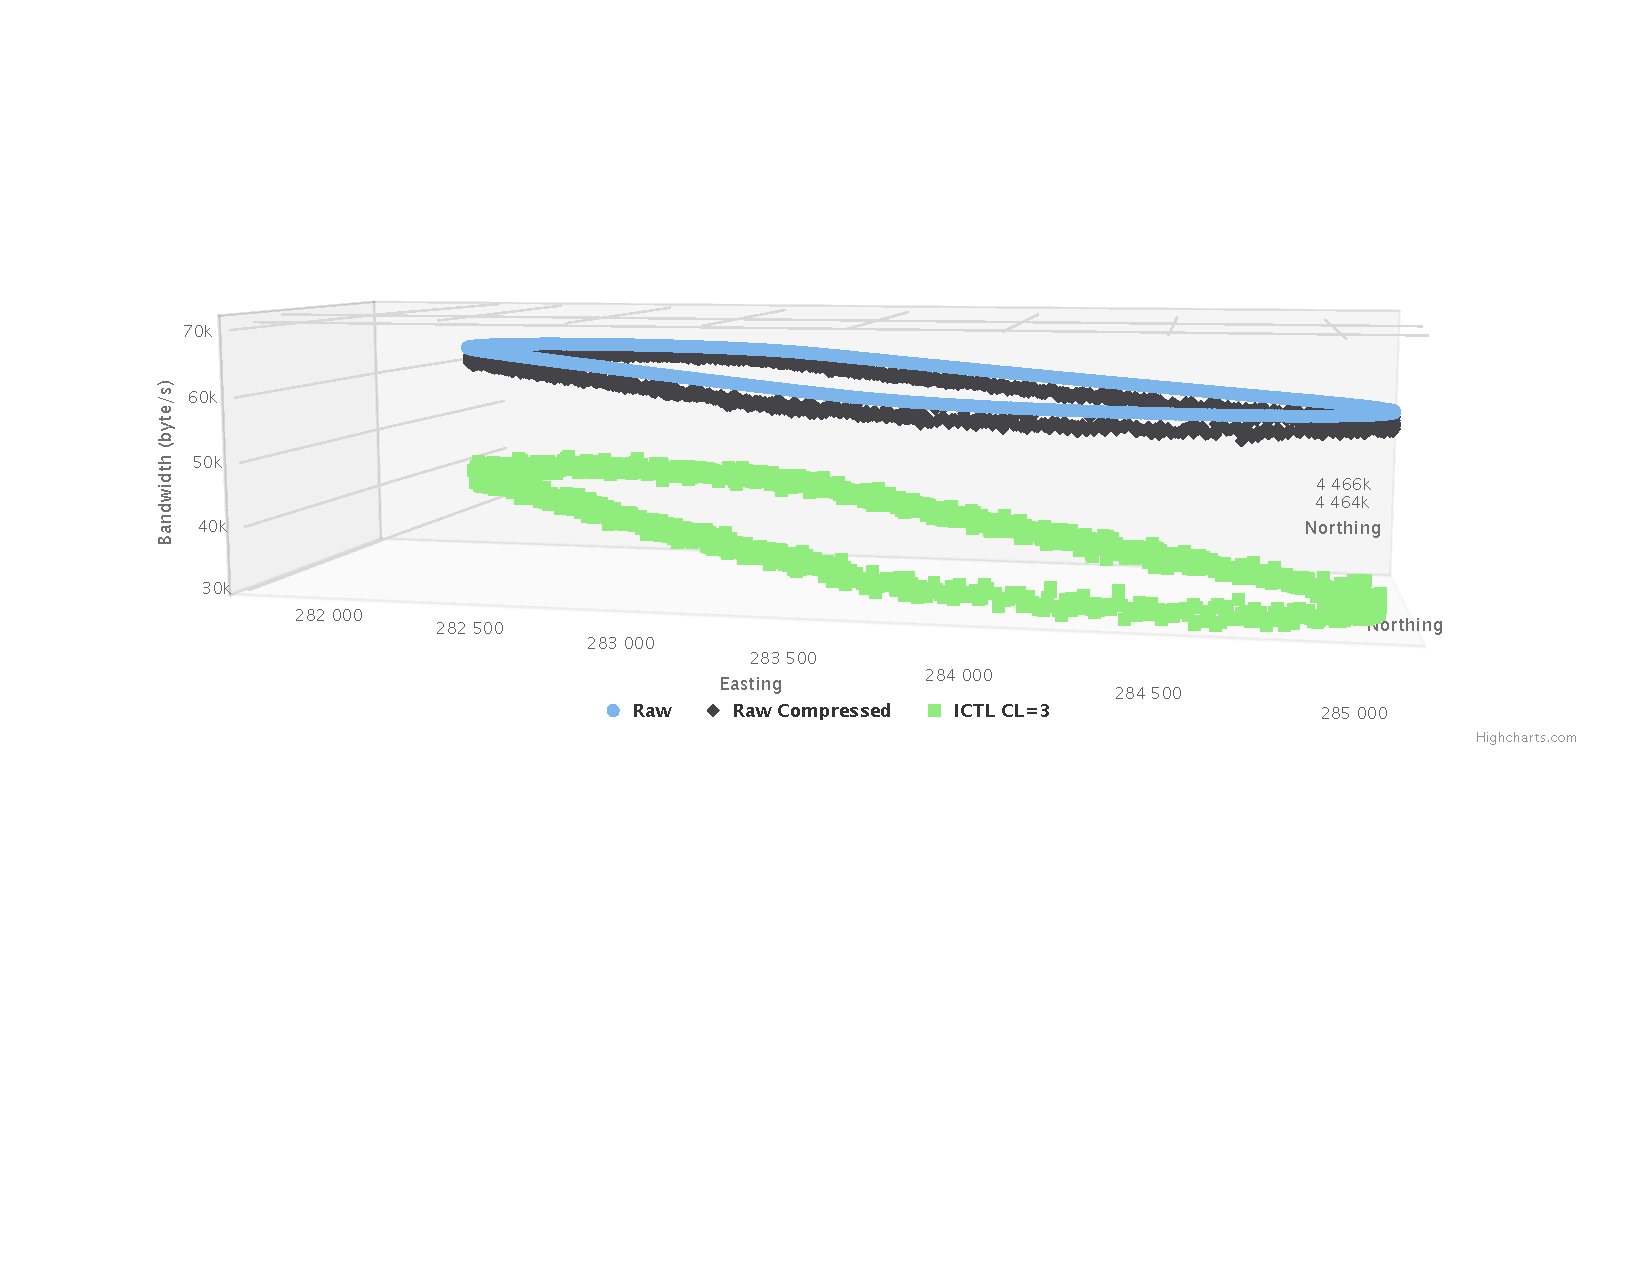
\includegraphics[width=1.1\textwidth]{figures/results/3d1.pdf}}
  \makebox[\textwidth][c]{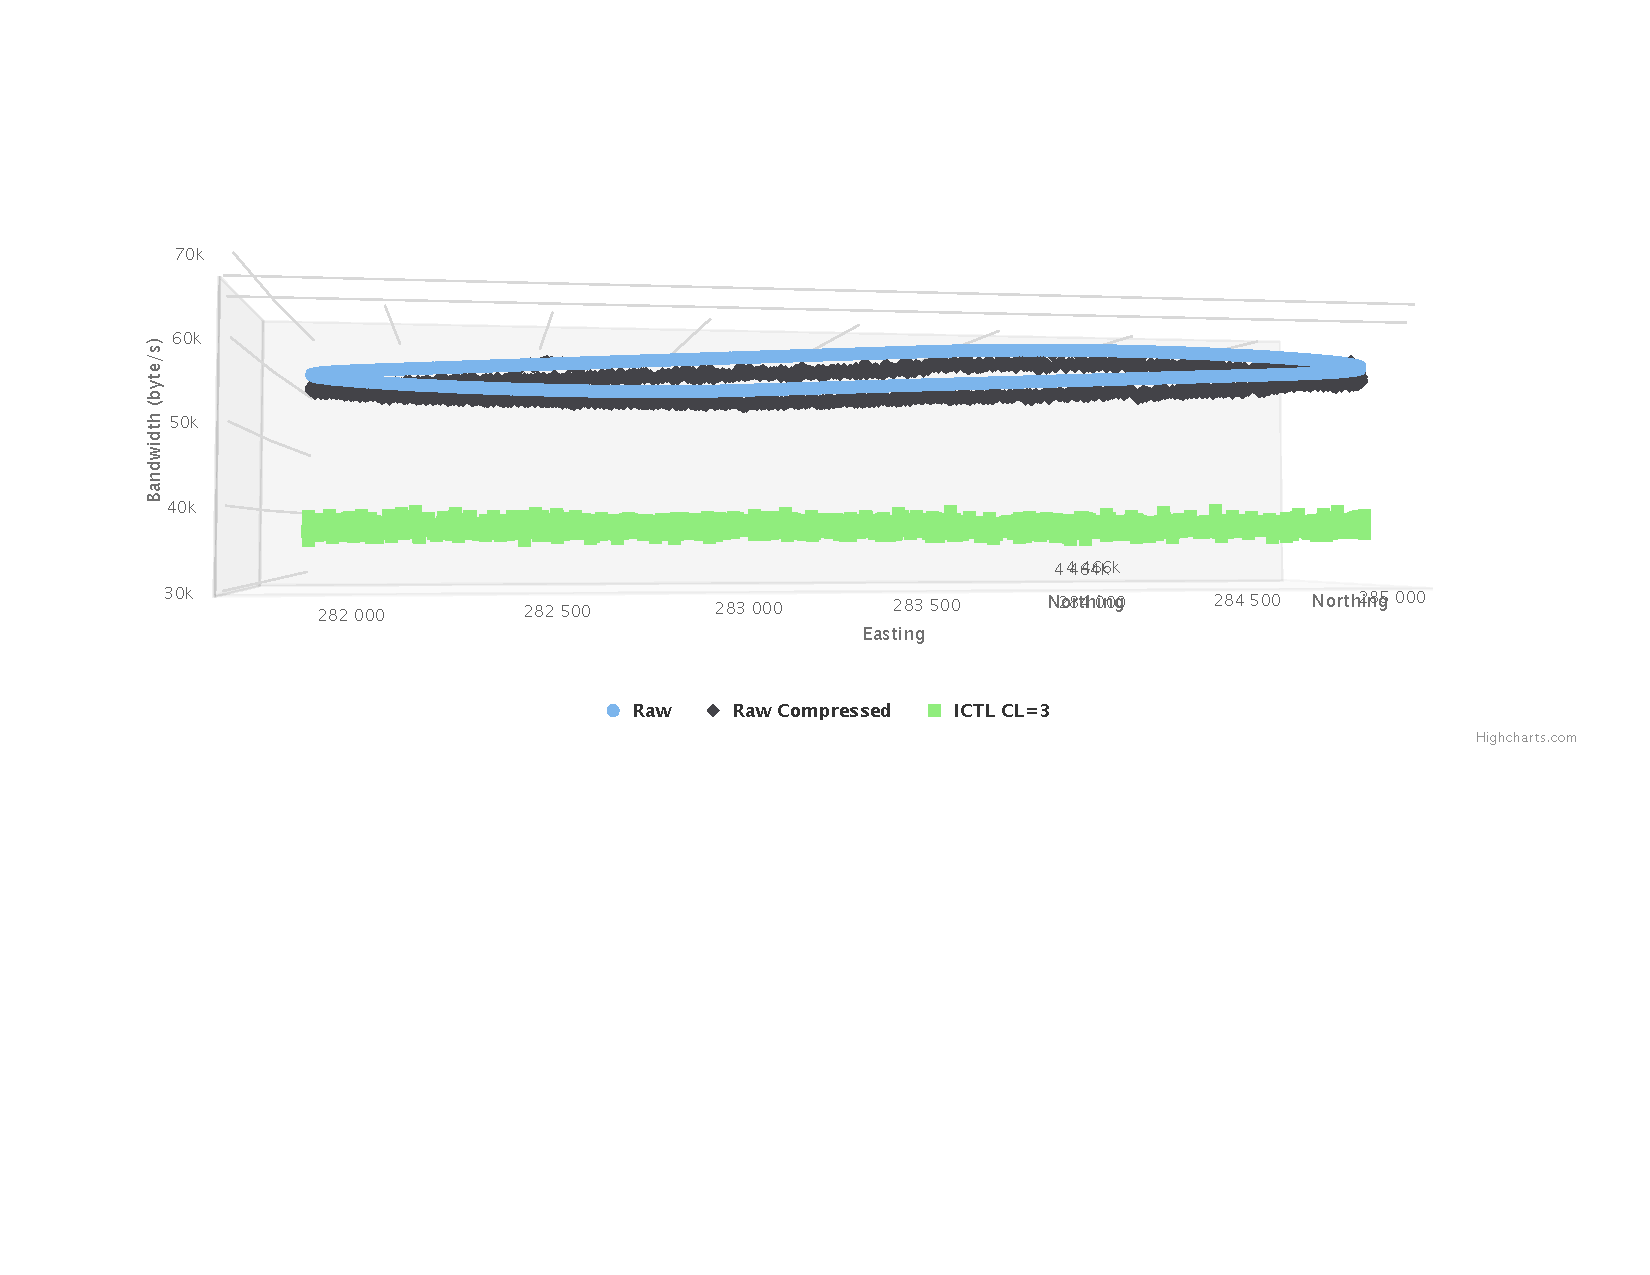
\includegraphics[width=1.1\textwidth]{figures/results/3d2.pdf}}
  \caption{\label{fig:3d}3D bandwidth graph from two viewing angles}
\end{figure}

As shown in the figure, ICTL does not generate more demanded bandwidth at curves. We believe this is because the changes of vehicle status at curves are gradual and slow enough to not cause drastic change in DSRC messages. Thus, they are not reflected in ICTL bandwidth consumption.

\subsection{Cycle Length and Bandwidth}
\label{sec:cl_bandwidth}

CL affects demanded bandwidth in a major, but complex way. DFs are generally much smaller than KFs. But the actual size of a DF depend on how different it is from the KF it uses as the reference frame. On one hand, since DFs are smaller, more DFs should be sent, thus longer CL is better. On the other hand, longer CL means the DFs towards the end of an ICTL Cycle is much more different from the KF, increasing size of DFs. As a result, longer CL does not always result in lower demanded bandwidth.

\begin{figure}[h]
  \makebox[\textwidth][c]{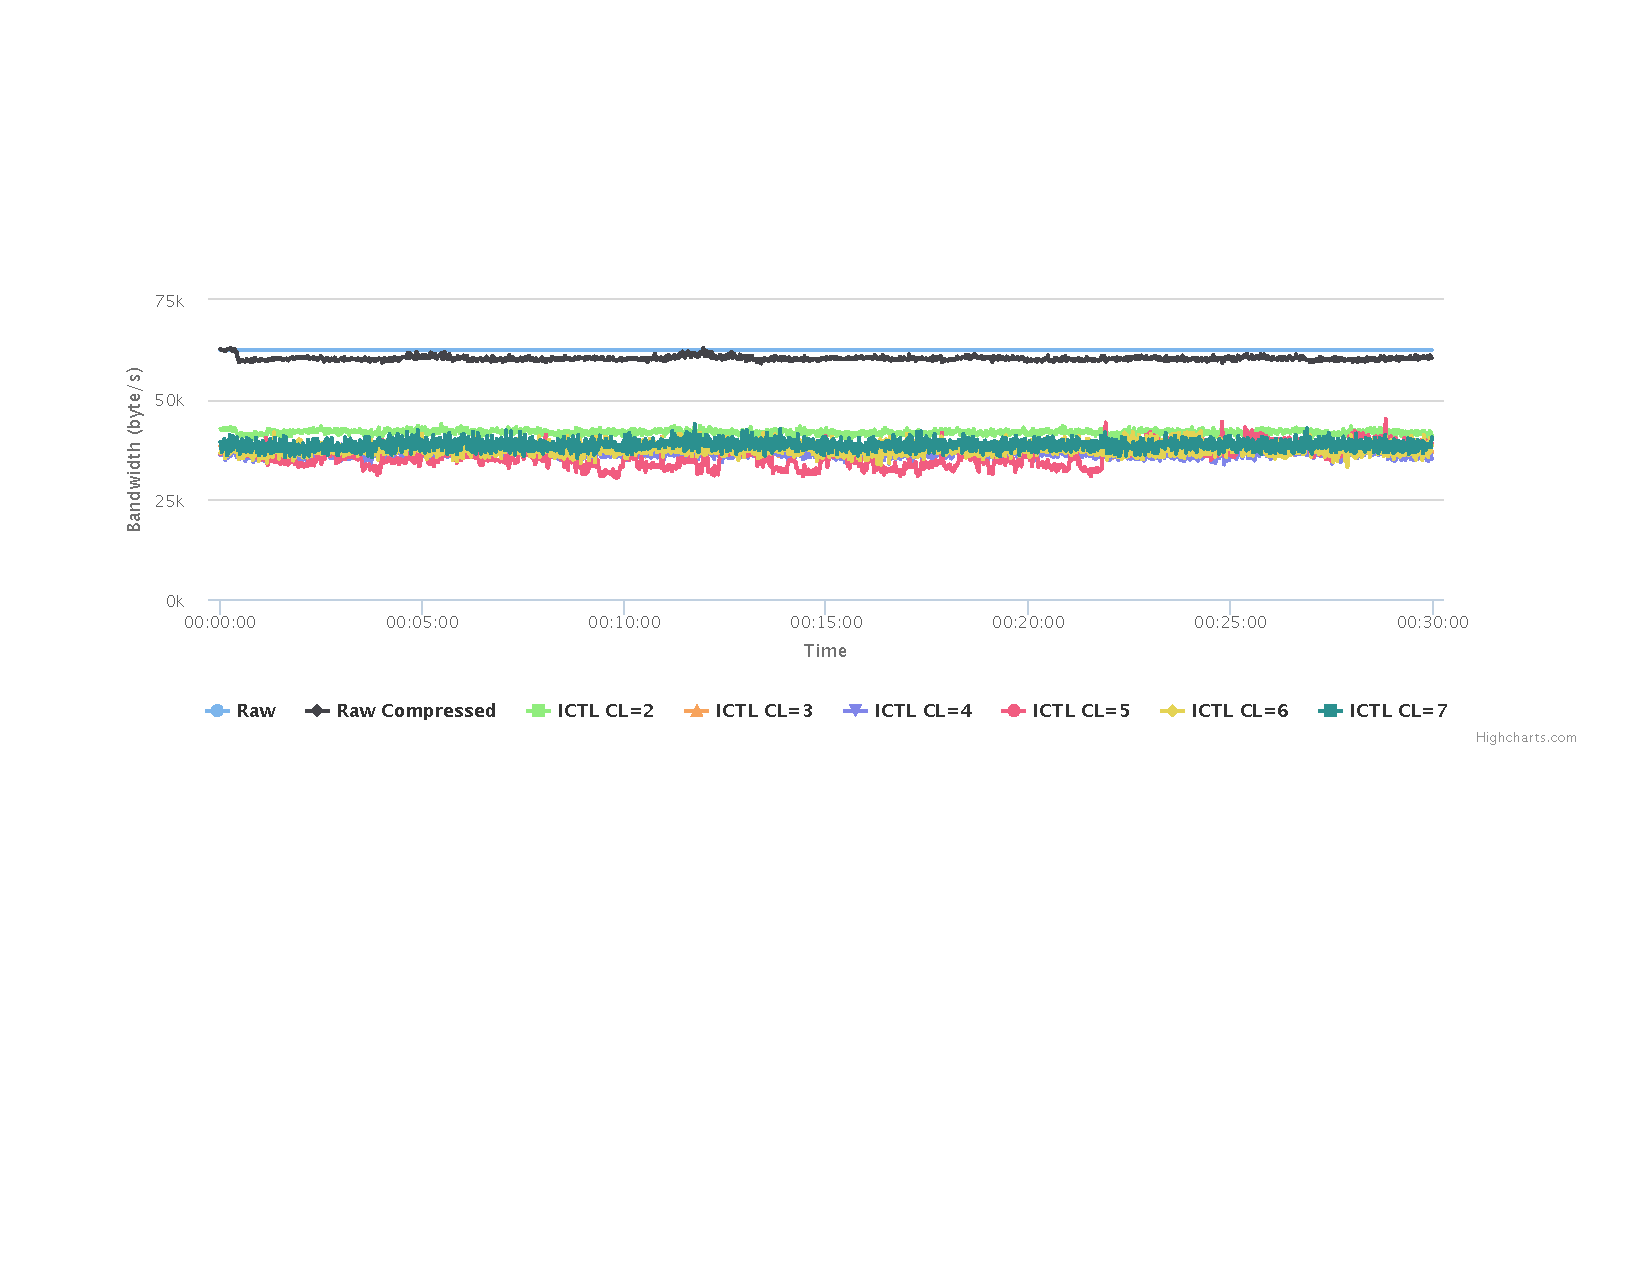
\includegraphics[width=1.1\textwidth]{figures/results/cycle_length.pdf}}
  \makebox[\textwidth][c]{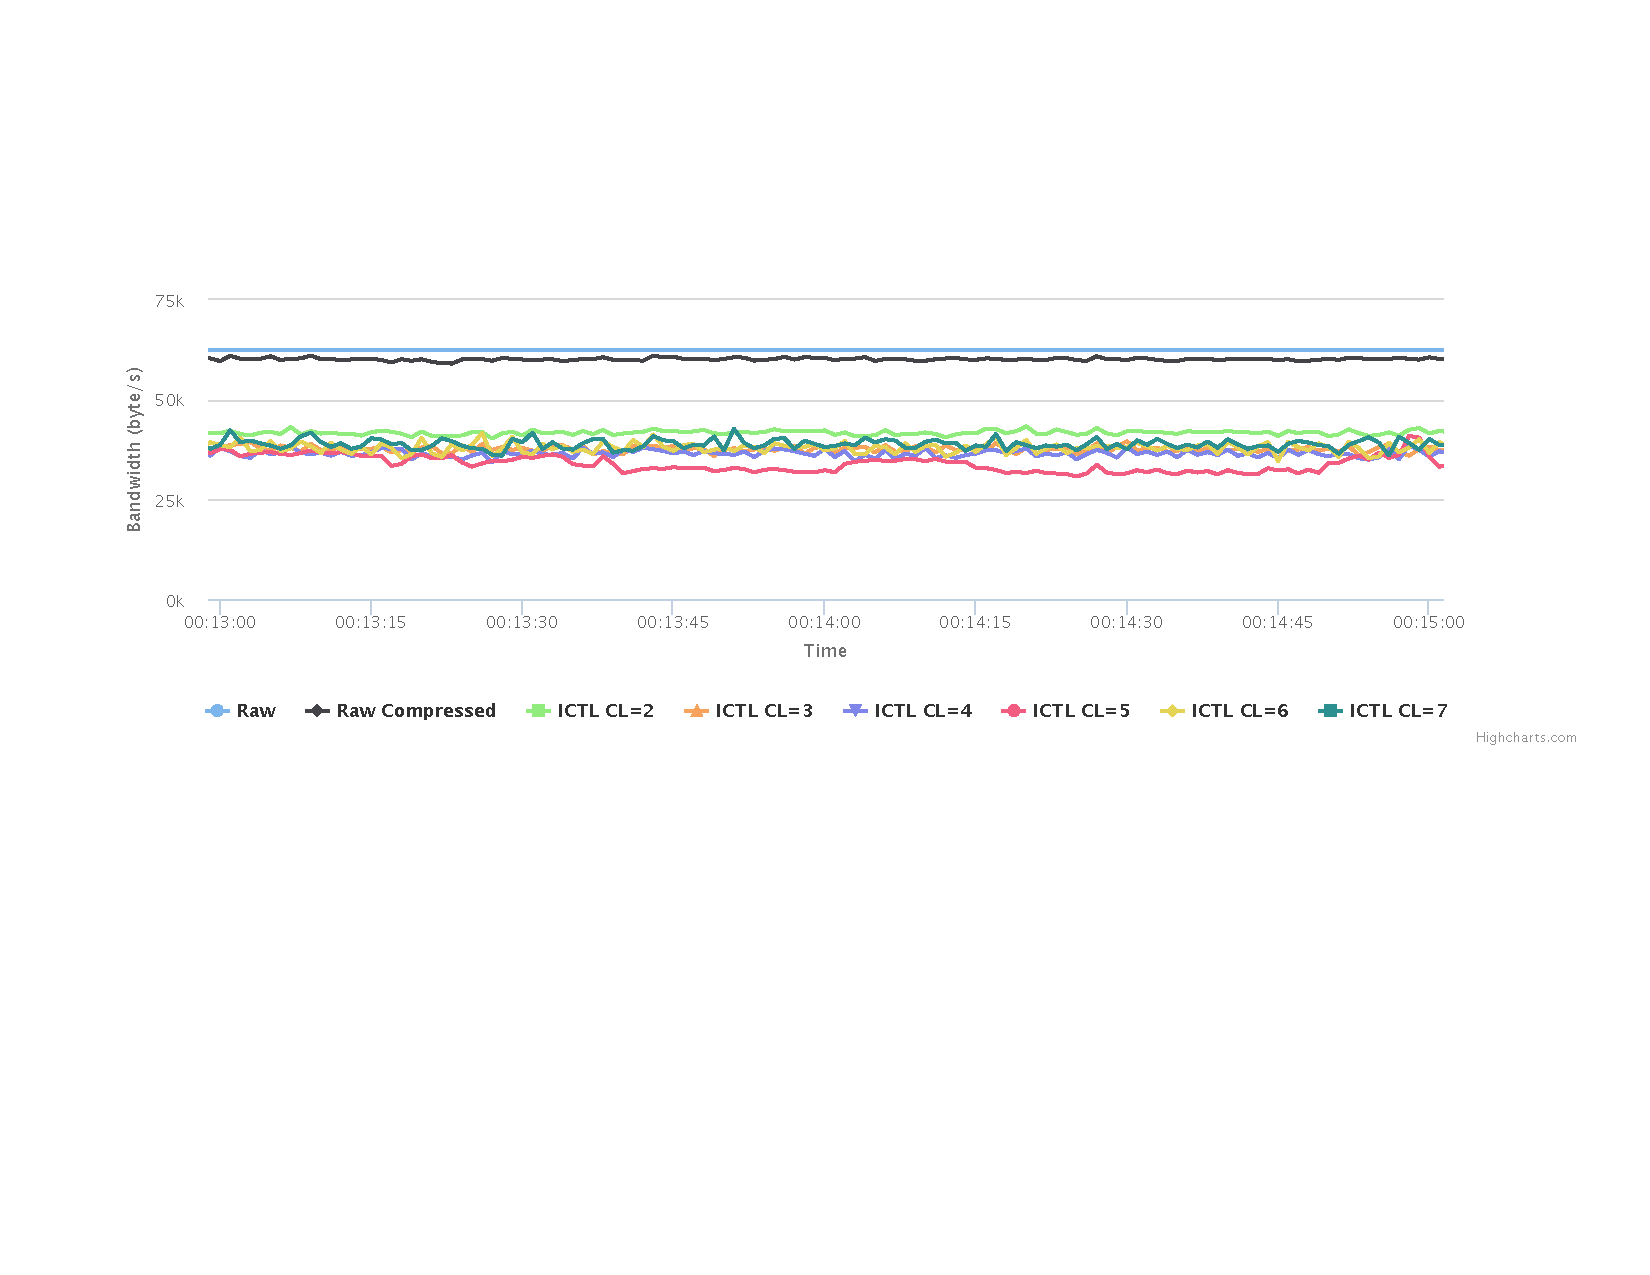
\includegraphics[width=1.1\textwidth]{figures/results/cycle_length_zoom.pdf}}
  \caption{\label{fig:cl}Bandwidth with different CL: 30-minute view and 2-minute zoom-in view}
\end{figure}

This theory is verified by tests. Figure~\ref{fig:cl} shows demanded bandwidth of ICTL with different fixed CLs, using the same data trace. Apparently when CL is set to 7, the demanded bandwidth is, in most of time, higher than when CL is set to 5, but they are both generally lower than when CL is set to 2. Furthermore, different data series cross each other, meaning that even for the same data trace, there is no CL setting that works the best all the time.

This shows that, it is challenging to set a proper fixed CL, and that with a fixed CL, ICTL is unable to always yield low demanded bandwidth. With this in mind, an adaptive algorithm is designed, as described in Section~\ref{sec:adaptive_ictl}.

\subsection{Payload Compression}
\label{sec:payload_compression}

ICTL has a header field of Compression Options, which carries information on how the payload is compressed before transmitted. This allows the receiver dynamically configure the decoder based on the header, and accept different compression algorithms and configurations. The compression algorithm used to compress DF payload affects overall size of DFs, so it is important to use one that performs well for such data.

At the beginning of this study, it was believed that, for different DFs, the best performing compression algorithm should be different. In other words, there should be no algorithm that worked for all DFs. As a result, a mechanism was designed in the ICTL implementation that, if the compression algorithm was not specified, it would iterate through a predefined selection of algorithms, and pick the one that yields smallest compressed payload.

\begin{figure}[htb]
  \makebox[\textwidth][c]{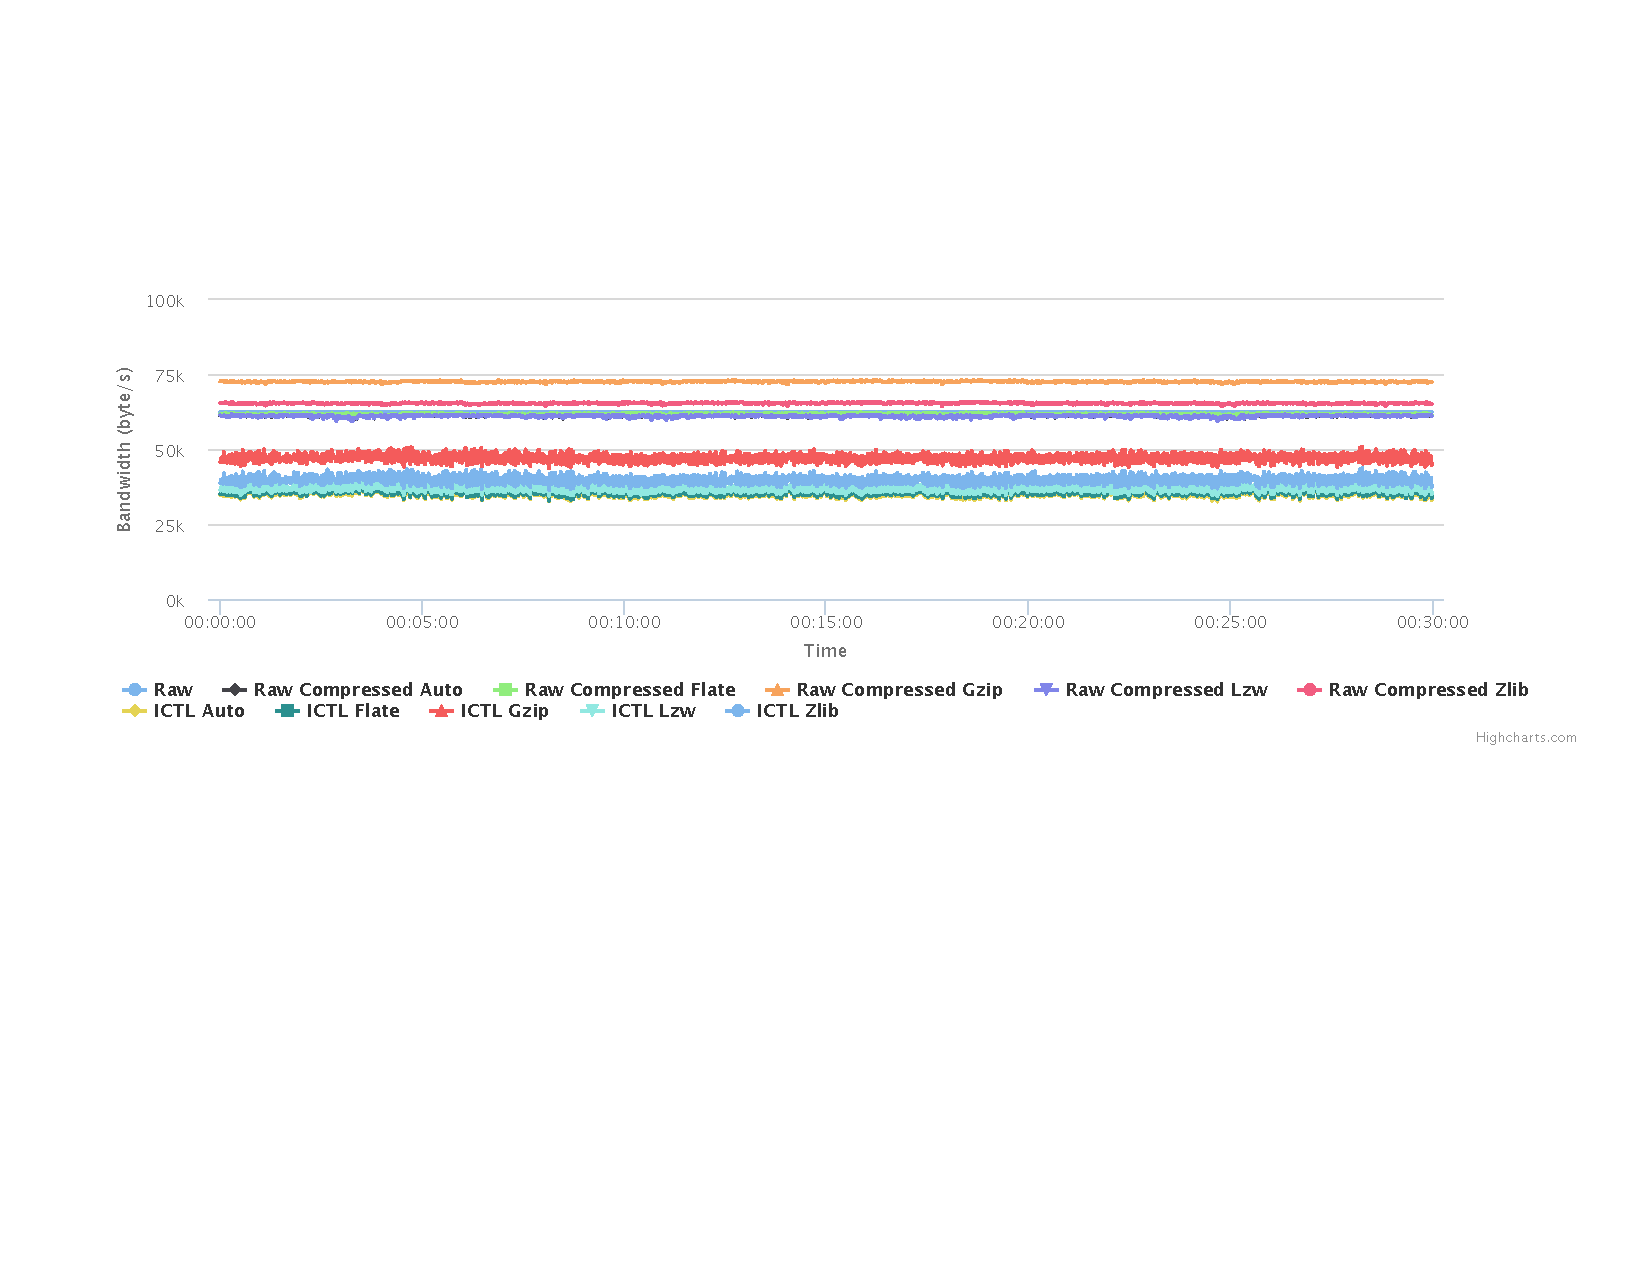
\includegraphics[width=1.1\textwidth]{figures/results/cmp.pdf}}
  \makebox[\textwidth][c]{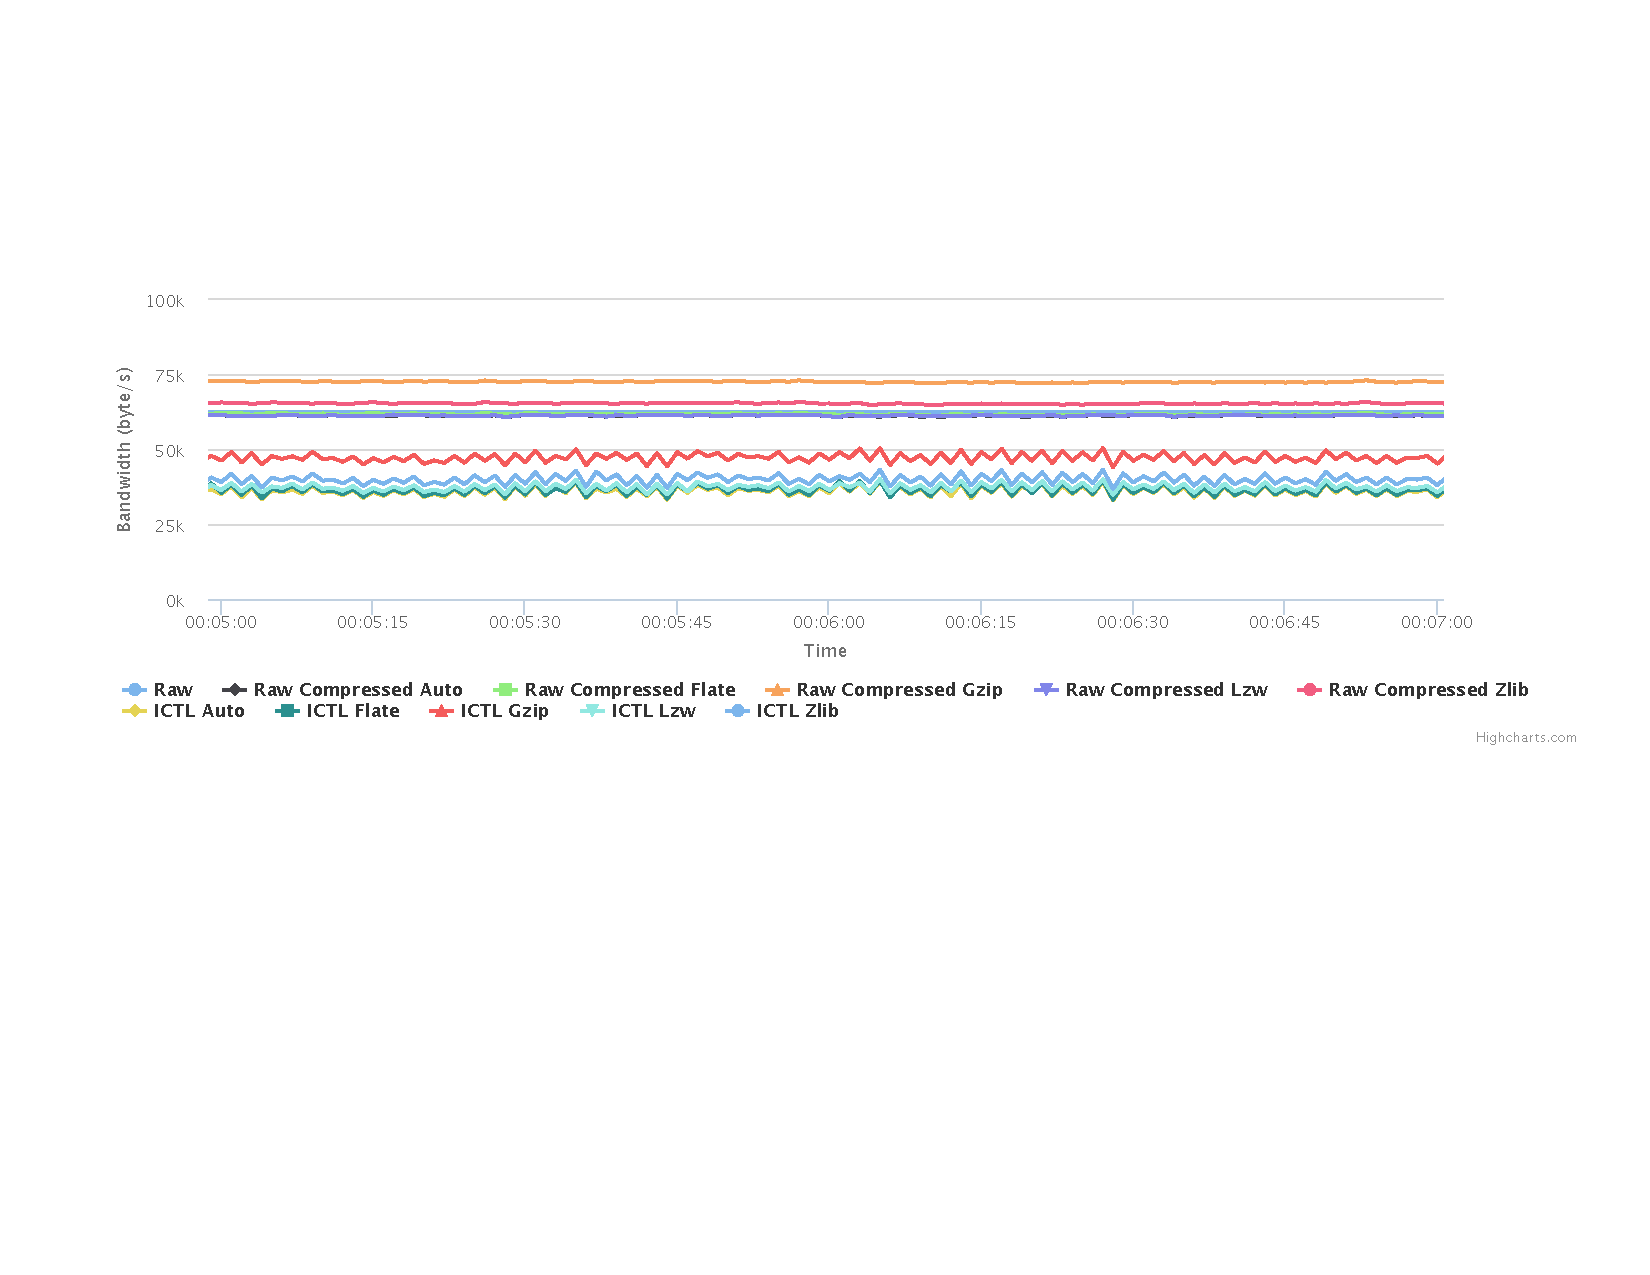
\includegraphics[width=1.1\textwidth]{figures/results/cmp_zoom.pdf}}
  \caption{\label{fig:cmp}Bandwidth with different payload compression algorithms: 30-minute view and 2-minute zoom-in view}
\end{figure}

To find out whether it makes sense to do so, tests are done to compare different compression algorithms for payload of frames. Specifically, \texttt{flate}, \texttt{zlib}, \texttt{gzip}, \texttt{lzw} are tested. Figure~\ref{fig:cmp} presents the results of the tests, which is contradictory to what was expected. Different data series generally do not cross each other, meaning their performance is fairly stable across different DFs. Among the four algorithms, \texttt{flate} and \texttt{lzw}, always yield smallest compressed payloads, with \texttt{flate} being slight better most of time.

Interestingly, \texttt{zlib} and \texttt{gzip} produces larger data than uncompressed. This suggests that \texttt{zlib} and \texttt{gzip} have compressing header overheads that are large enough to make them not suitable for compressing small size data, thus should not be directly used to compress payload of KFs and DFs.

Guided by findings here, the rest of tests in this study use \texttt{flate} in ICTL.

\section{Adaptive ICTL}
\label{sec:adaptive_ictl}

Section~\ref{sec:cl_bandwidth} shows that a fixed CL cannot constantly perform well in terms of bandwidth consumption. In other words, CL should be chosen dynamically as ICTL is running. Looking at this from a different perspective, CL is merely the observed behavior of ICTL. What should be determined dynamically is actually, at any given time, whether ICTL should send a DF, i.e., continue within the same ICTL Cycle, or a KF, i.e., start a new ICTL Cycle. The \texttt{shouldDF()} function in Section~\ref{sec:ictl_process} is where this decision is made.

This sections describes an adaptive ICTL algorithm, in which a \texttt{shouldDF()} is designed to optimize for bandwidth consumption.

\subsection{Design}

In an imaginary world where a node knows exactly what it will be transmitting for sufficiently large amount of time, and there are usable quantum computers that make it viable to exhaust large search space, this would be an optimization problem where the goal is to find globally optimal sequence of CLs for the entire transmission consisting all frames, that produces the lowest bandwidth consumption throughout the transmission. However, in real-world, ICTL is in no way able to predict what will be transmitted, and the node has limited hardware resources for searching for optimal solution. What ICTL can do is to look at locally available information, and make the best decision for bandwidth consumption based on a well selected metric. 

In this study, ICTL uses a metric of average frame size of the ICTL Cycle up to the moment. More formally, for each frame being transmitted, the metric $\mu_{cycle}$ for $n$th frame within the ICTL Cycle is defined as Equation~\ref{eq:mu_cycle}:

\begin{equation}
  \mu_{cycle}^n = \frac{S_{KF} + \sum_{i=2}^{n}{S_{DF}^i}}{n}
  \label{eq:mu_cycle}
\end{equation}

, where $S$ is the size of corresponding frame, and $i$ is the frame number within the ICTL Cycle. $i$ is greater than or equal to 2, because the first frame in an ICTL Cycle is always a KF.

$\mu_{cycle}^x$ is the key metric used by ICTL to determine whether a DF should be used for $x$th frame in the ICTL Cycle. First of all, ICTL keeps track of the immediately previous calculated metric, $\mu_{cycle}^{x-1}$. When ICTL transmits a frame $x$, it first encodes a DF, and inspects its size $S_{DF}^x$, with which $\hat{\mu}_{cycle}^x$ is calculated according to Equation~\ref{eq:mu_cycle}. If $\hat{\mu}_{cycle}^x < \mu_{cycle}^{x-1}$, it implies that, by sending another DF in this ICTL Cycle, the average frame size within the cycle can be further reduced, so ICTL should send a DF for this frame. In this case, $\hat{\mu}_{cycle}^x$ becomes $\mu_{cycle}^x$, and the DF is sent. Otherwise, a KF is sent, and a new ICTL Cycle is started.

Following is a pseudo-code listing for logic to determine whether a DF should be sent, using Go-like syntax:

\begin{singlespace}
  \lstinputlisting{adaptive.go.lst}
\end{singlespace}

ICTL calls \texttt{sentDF()} and \texttt{sentKF()} methods whenever it sends a DF or a KF. It calls \texttt{shouldSendThisDF()} method to determine whether the next frame should be sent as DF or KF.

This algorithm minimizes average frame size within ICTL Cycle. Although it only utilizes local information, the optimization is a step towards optimized CLs and achieves much lower bandwidth consumption.

\subsection{Experimental Results}

Tests are conducted to verify the adaptive ICTL algorithm. Figure~\ref{fig:adaptive_bandwidth}. shows bandwidth consumption with adaptive ICTL, and basic ICTL with different fixed CL settings.

\begin{figure}[h]
  \makebox[\textwidth][c]{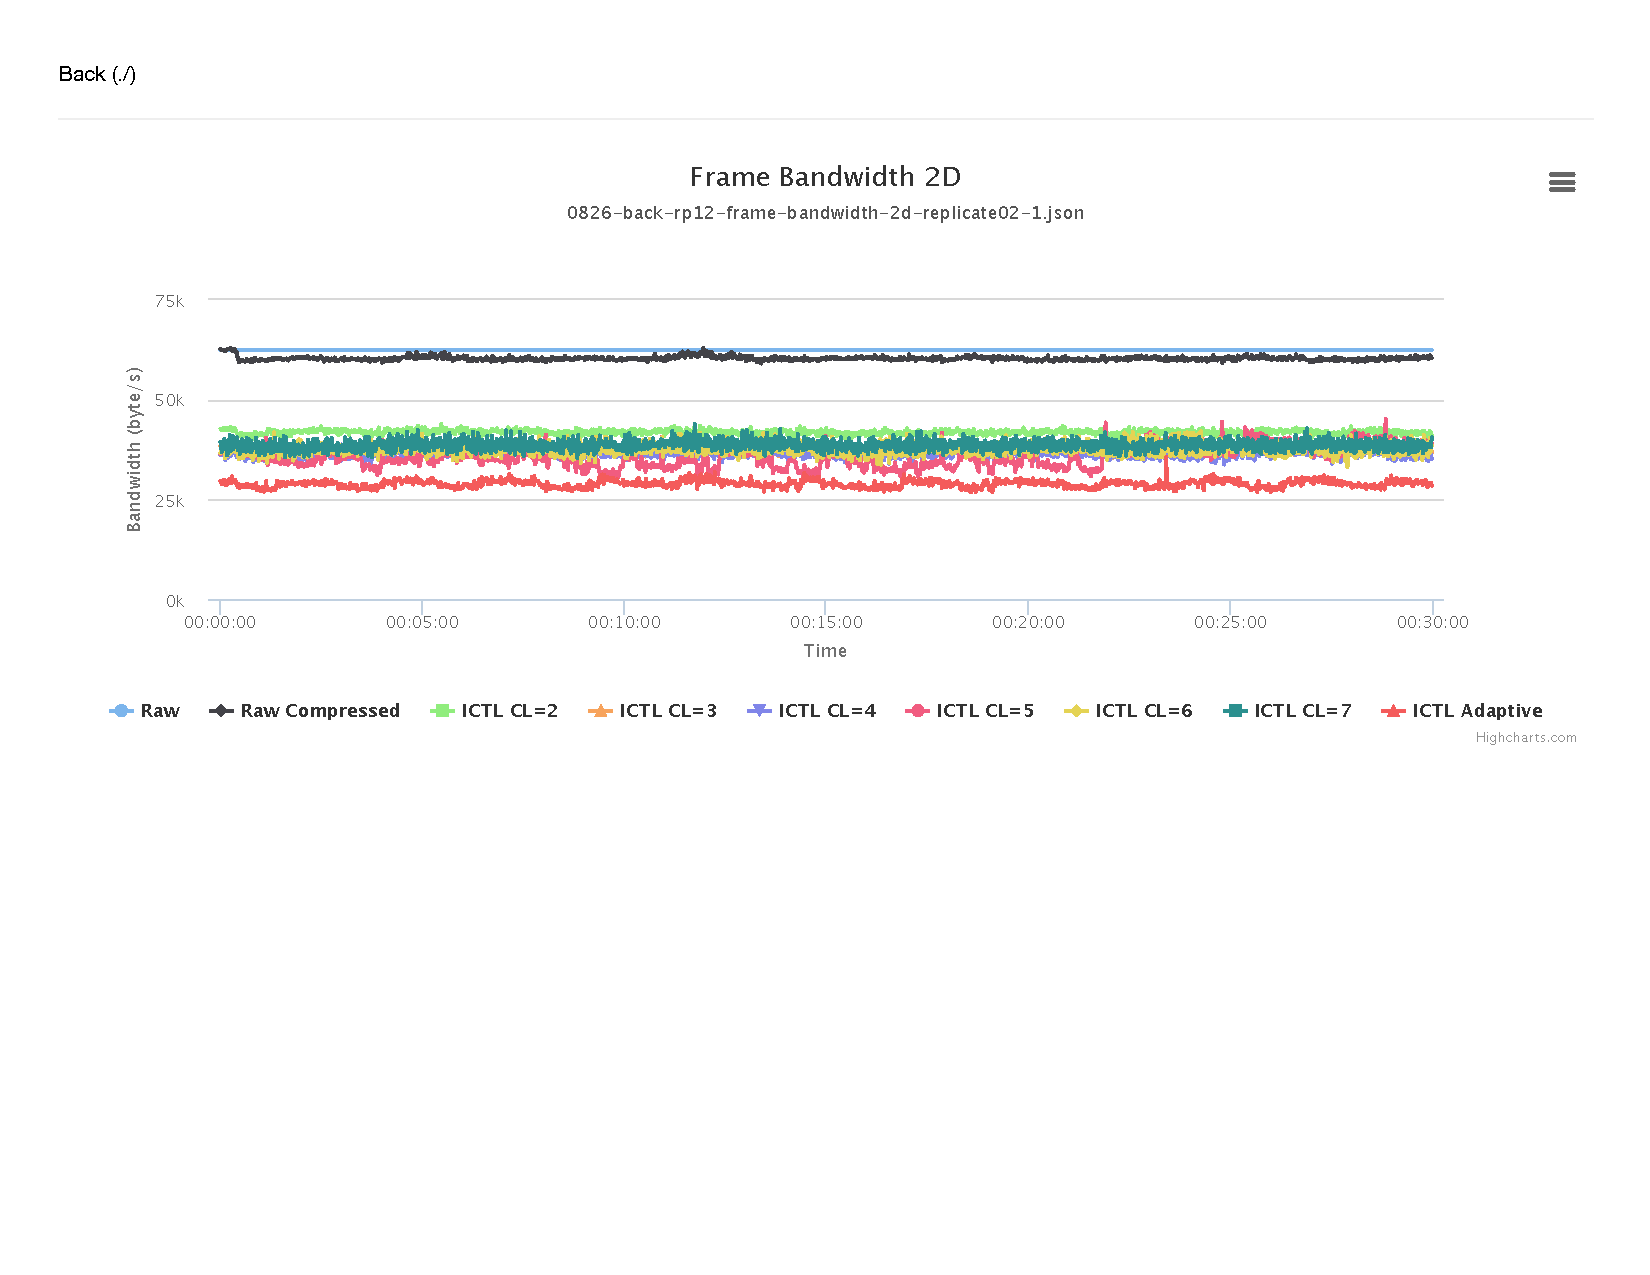
\includegraphics[width=1.1\textwidth]{figures/results/adaptive_bandwidth.pdf}}
  \caption{\label{fig:adaptive_bandwidth}Bandwidth consumption with adaptive ICTL and fixed CLs: 30-minute view}
\end{figure}

The figure shows that adaptive ICTL's bandwidth consumption is constantly the lowest among all data series. Furthermore, even the lowest one among fixed CLs is still 5 KB/s, or 15\% higher than adaptive ICTL. This verifies that a dynamic decision making process like adaptive ICTL works better than using a fixed CL, yielding much lower bandwidth consumption. Looking at absolute numbers, adaptive ICTL's bandwidth consumption stays below 30 KB/s most of time. Compared with original data trace which constantly consumes 62.5 KB/s bandwidth, adaptive ICTL yields more than 50\% bandwidth saving.

As discussed in Section~\ref{sec:cl_adr}, since NDR is the main affecting factor in ADR, and that bandwidth affects NDR in a major way, ICTL should optimize for bandwidth in order to achieve good ADR. To verify this, delivery ratio, specifically ADRs, of different congestion levels are studied as well. As explained in Section~\ref{sec:trigger_congestion}, messages are already replicated 12 times to make it easier to trigger congestion. Here different number of nodes are used to emulate different congestion level.

\begin{figure}[H]
  \makebox[\textwidth][c]{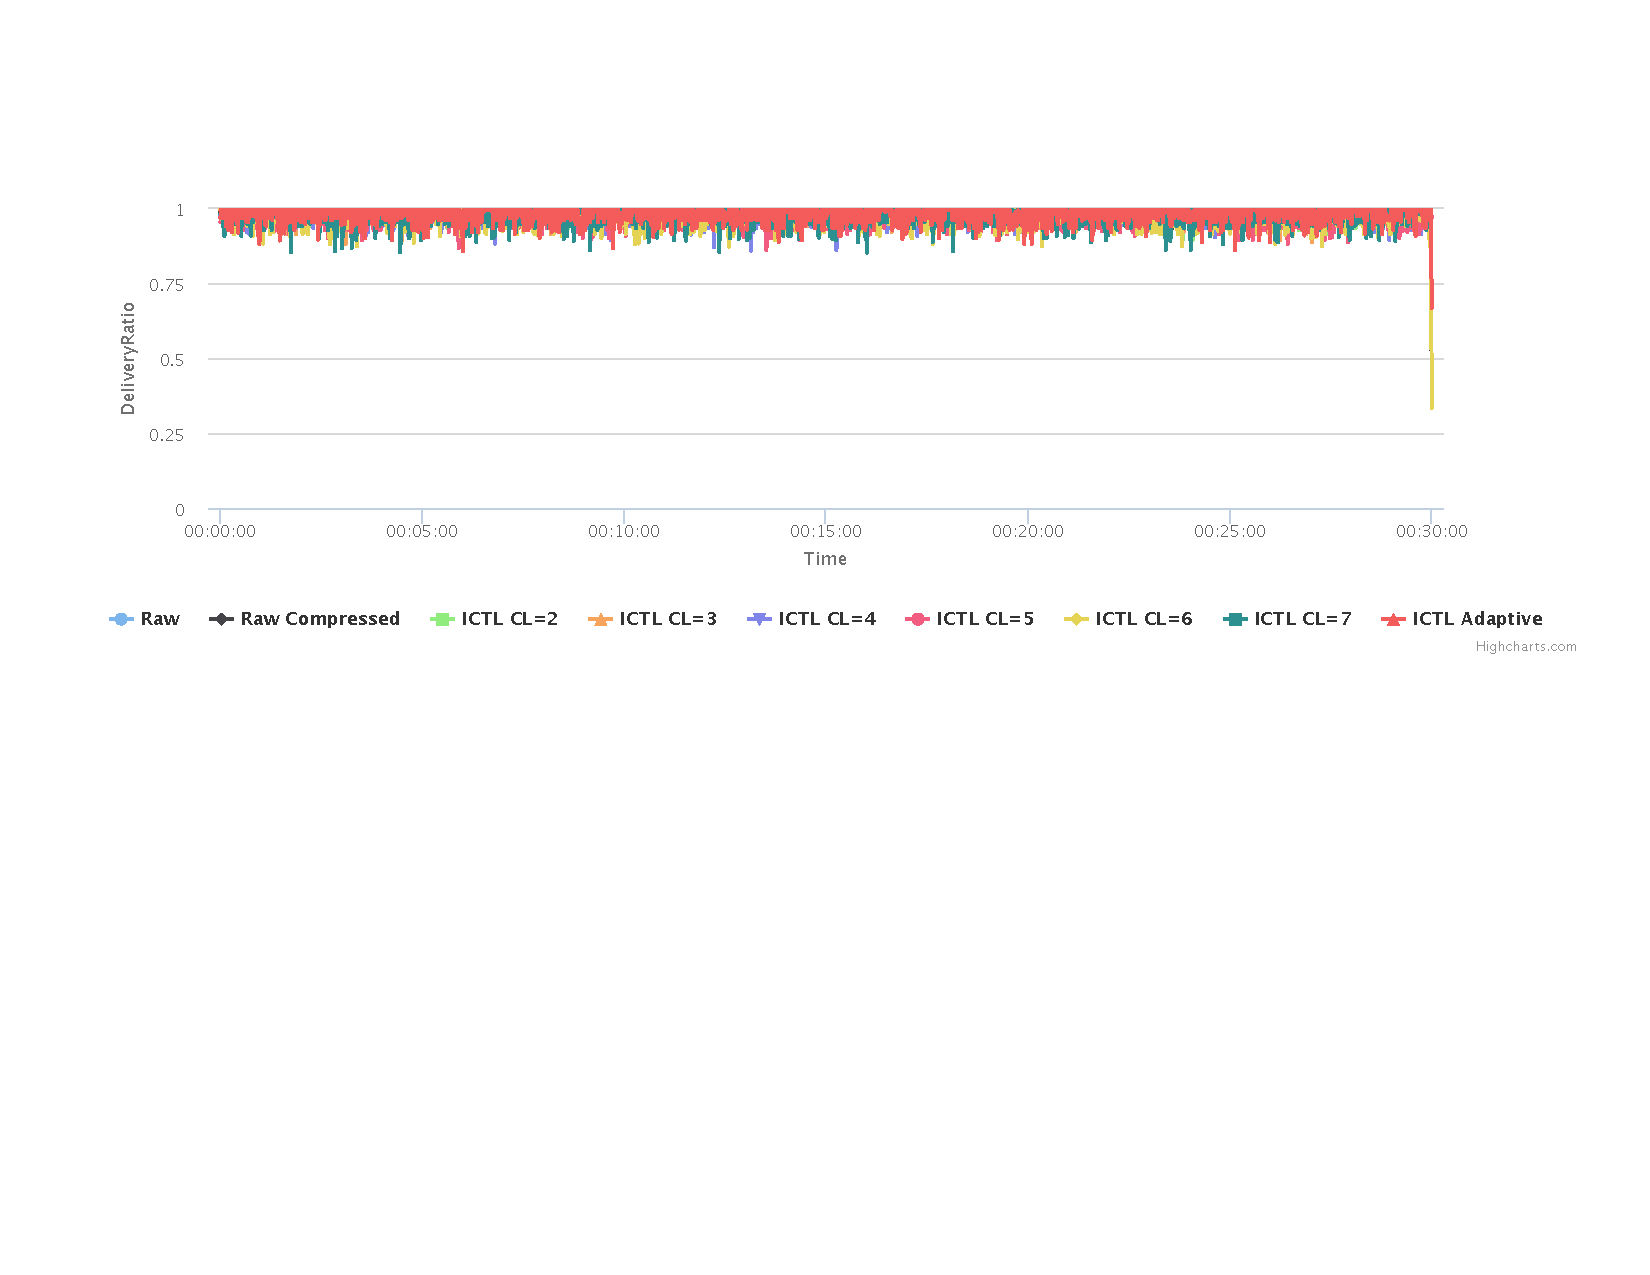
\includegraphics[width=1.1\textwidth]{figures/results/adaptive_adr-4.pdf}}
  \makebox[\textwidth][c]{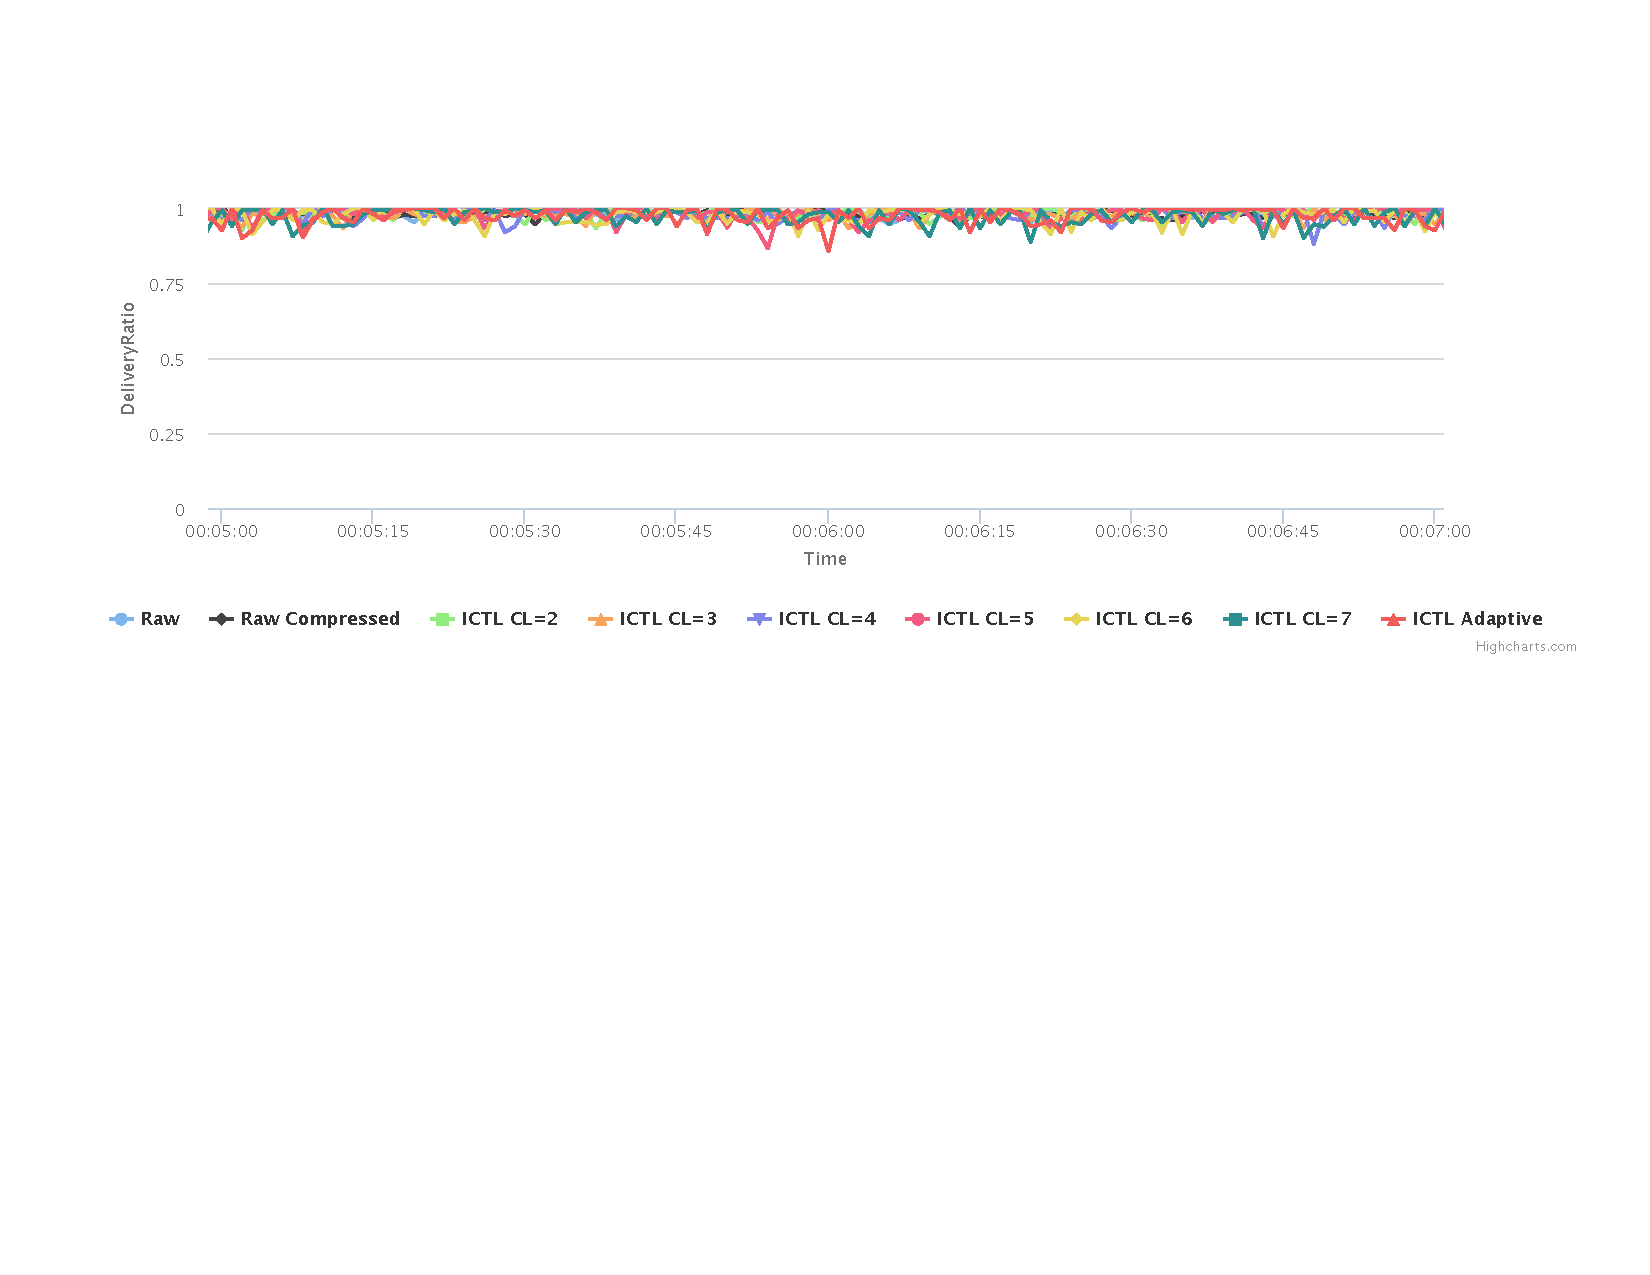
\includegraphics[width=1.1\textwidth]{figures/results/adaptive_adr-4_zoom.pdf}}
  \caption{\label{fig:adaptive_adr_4}ADR in adaptive ICTL compared other transmission strategies with 4 nodes: 30-minute view and 2-minute zoom-in view}
\end{figure}

Figure~\ref{fig:adaptive_adr_4} shows ADR for adaptive ICTL compared with other transmission strategies when there are 4 nodes in emulation. In this case, all data series show a good delivery ratio, close or equal to 100\%. Note that even congestion is not triggered for any transmission strategy in this case, there are still packet losses. This is because Squirrel's CSMA/CA model looks at leaky bucket usage, and uses a probability function based on it to determine whether a frame should be delivered. Arguably, this is emulating a realistic real-world experimental environment.

\begin{figure}[H]
  \makebox[\textwidth][c]{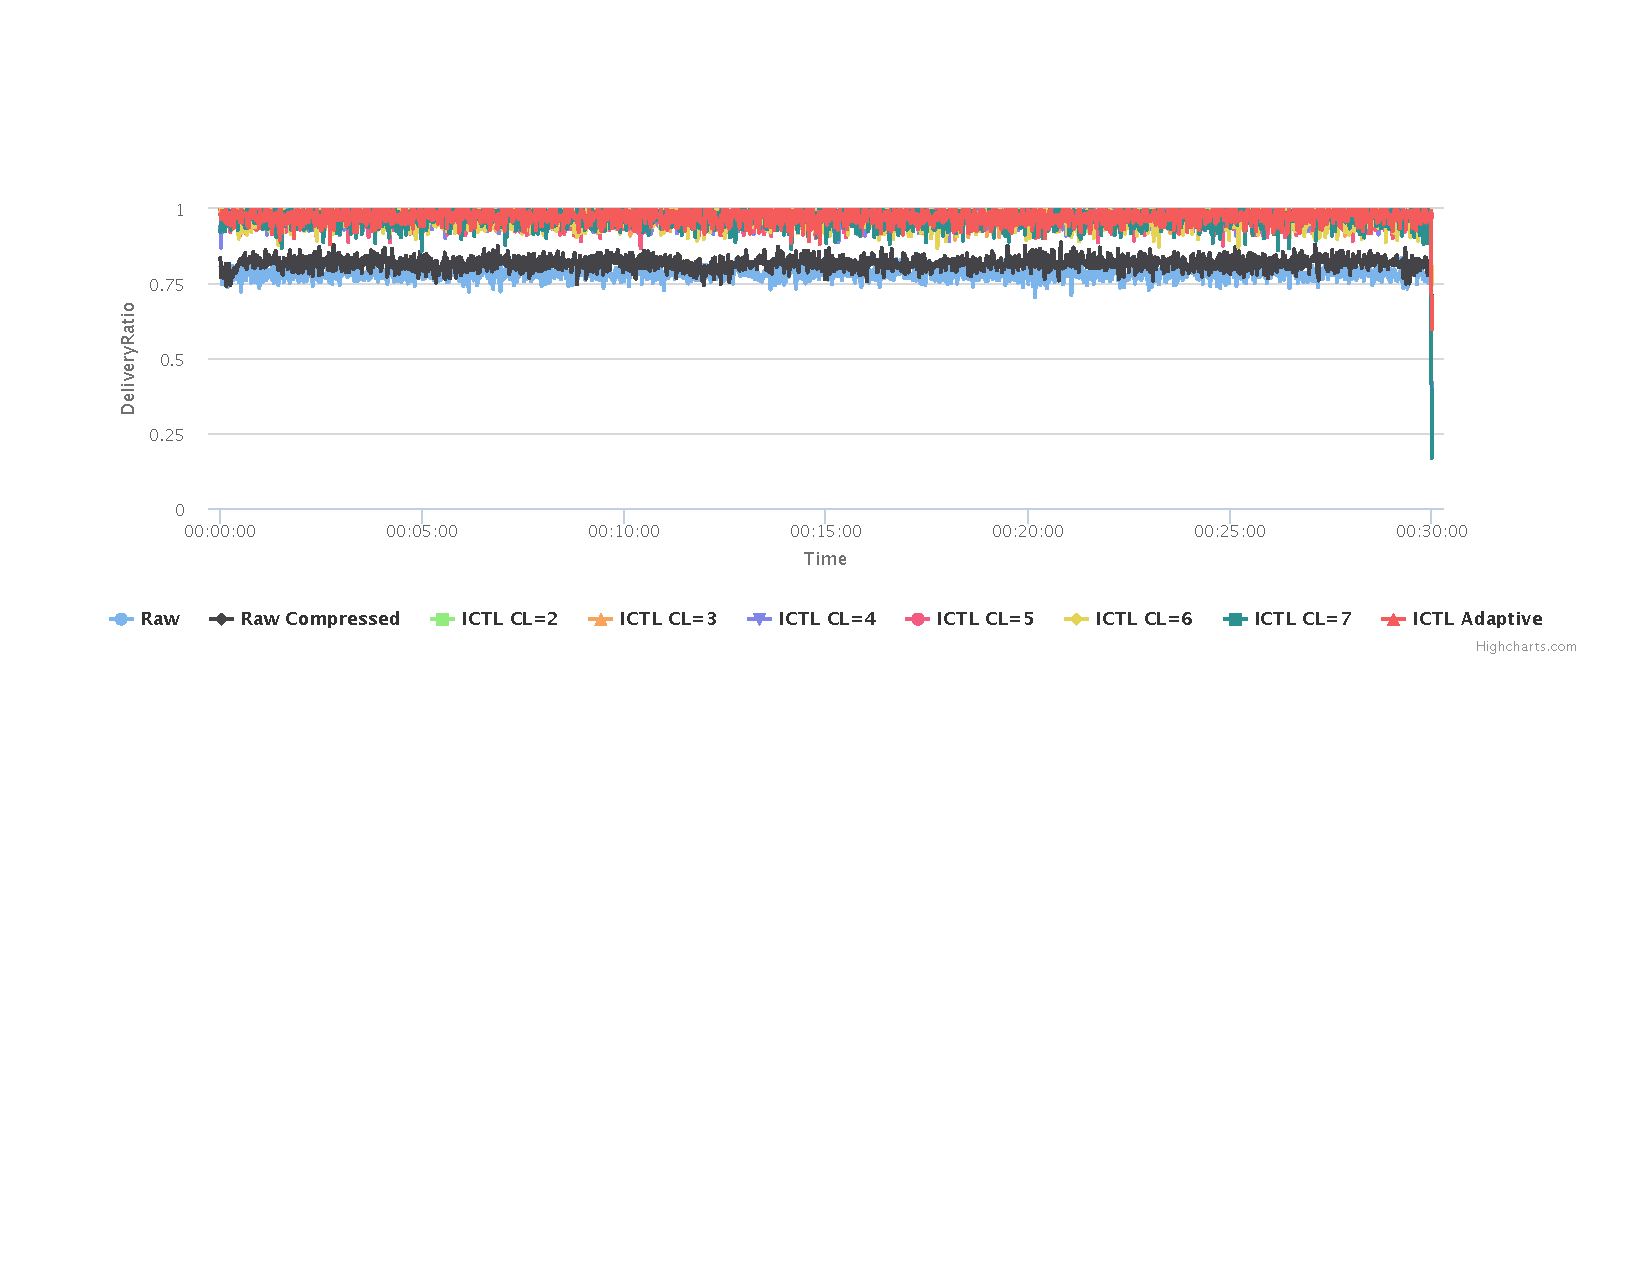
\includegraphics[width=1.1\textwidth]{figures/results/adaptive_adr-6.pdf}}
  \makebox[\textwidth][c]{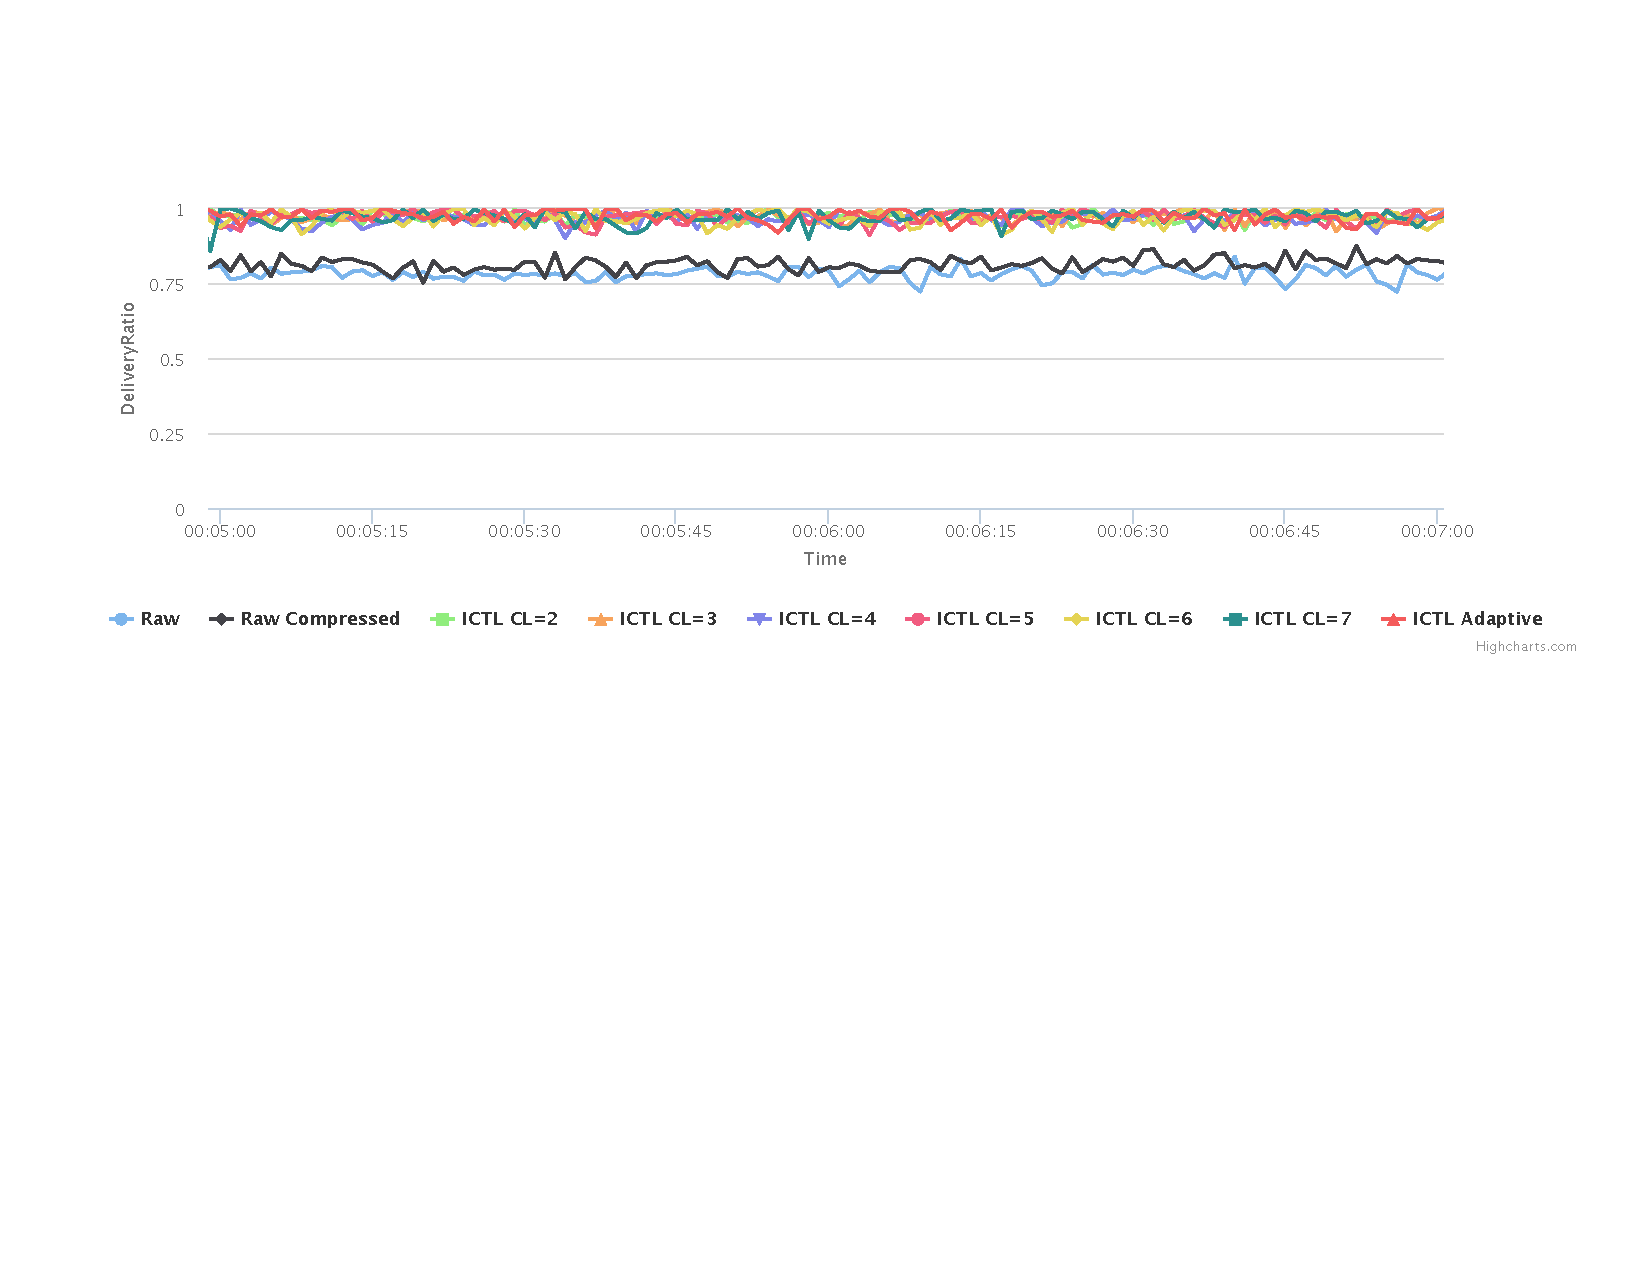
\includegraphics[width=1.1\textwidth]{figures/results/adaptive_adr-6_zoom.pdf}}
  \caption{\label{fig:adaptive_adr_6}ADR in adaptive ICTL compared other transmission strategies with 6 nodes: 30-minute view and 2-minute zoom-in view}
\end{figure}

Figure~\ref{fig:adaptive_adr_6} shows ADR results when there are 6 nodes in emulation. In this case, congestion starts to happen for original data trace as well as using traditional compression method. All ICTL compressed data series still have close or equal to 100\% ADR.

\begin{figure}[H]
  \makebox[\textwidth][c]{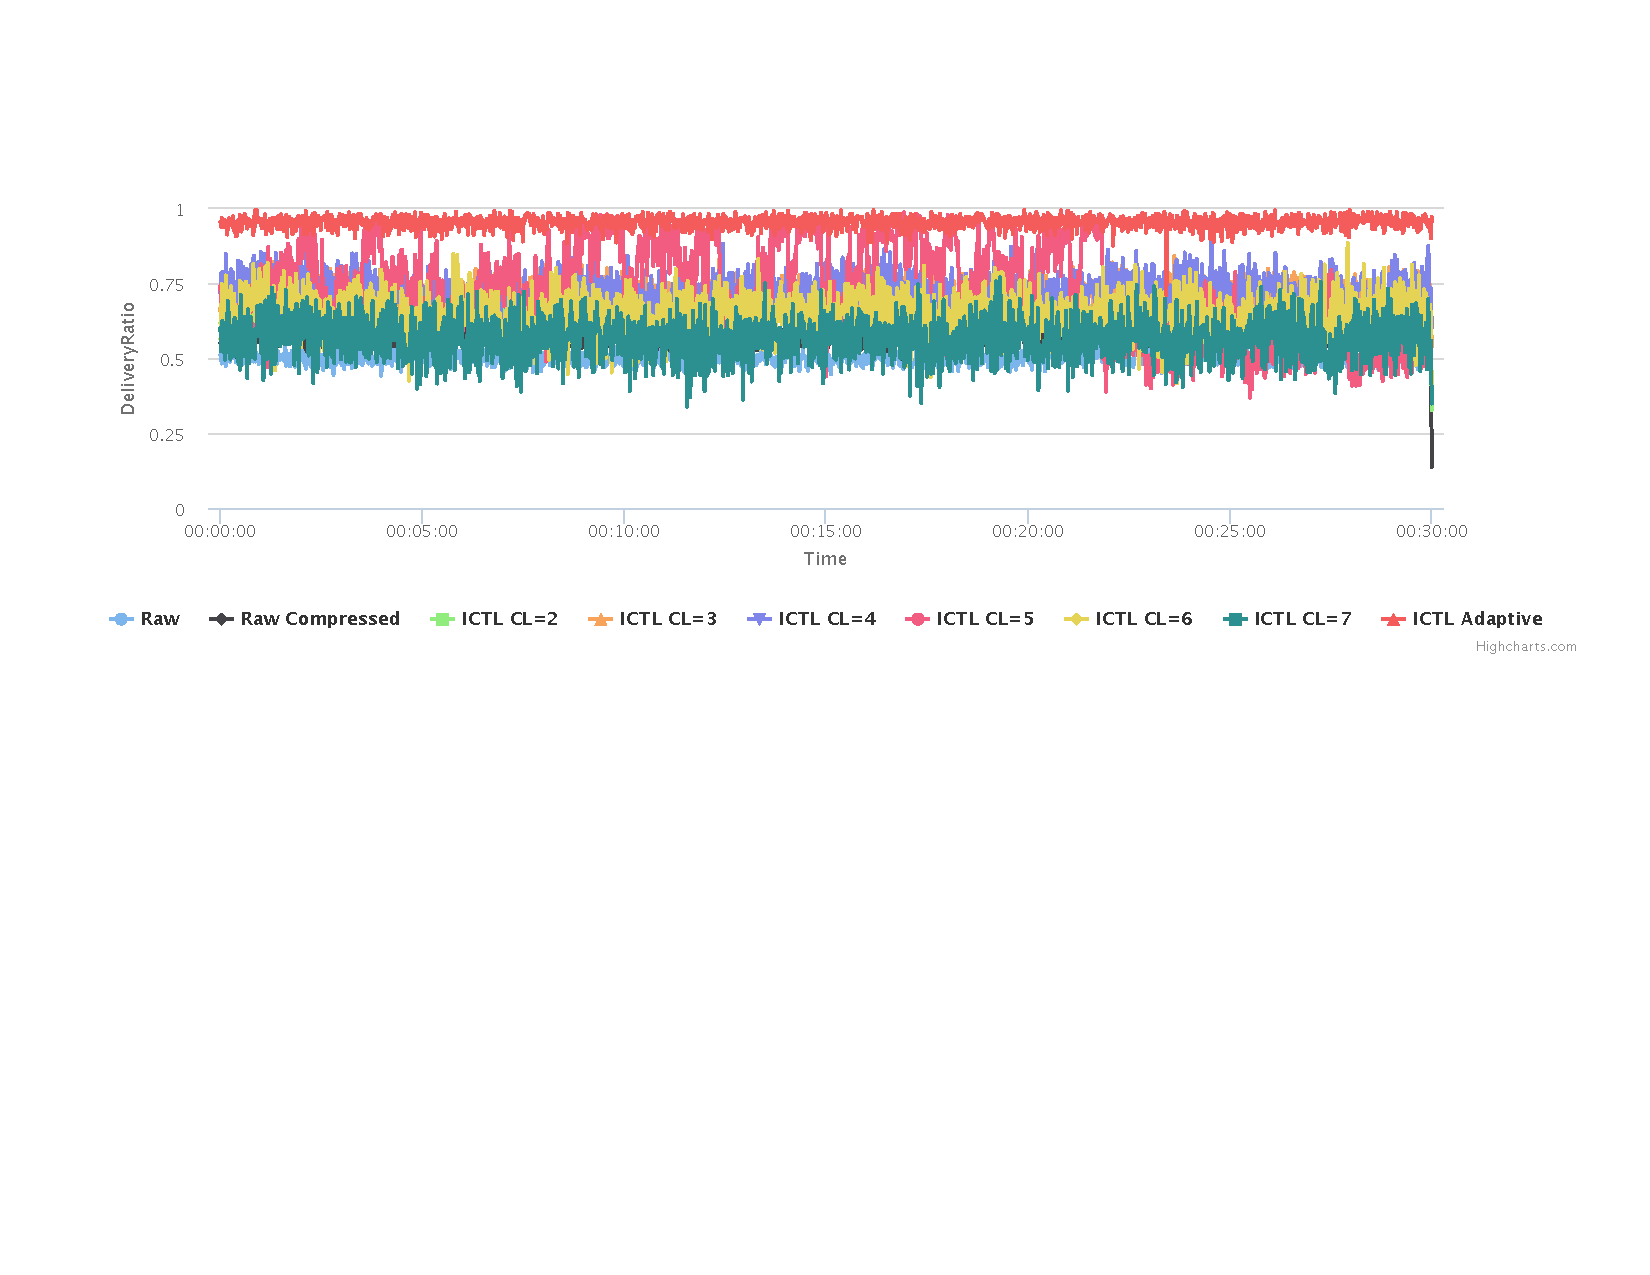
\includegraphics[width=1.1\textwidth]{figures/results/adaptive_adr-10.pdf}}
  \makebox[\textwidth][c]{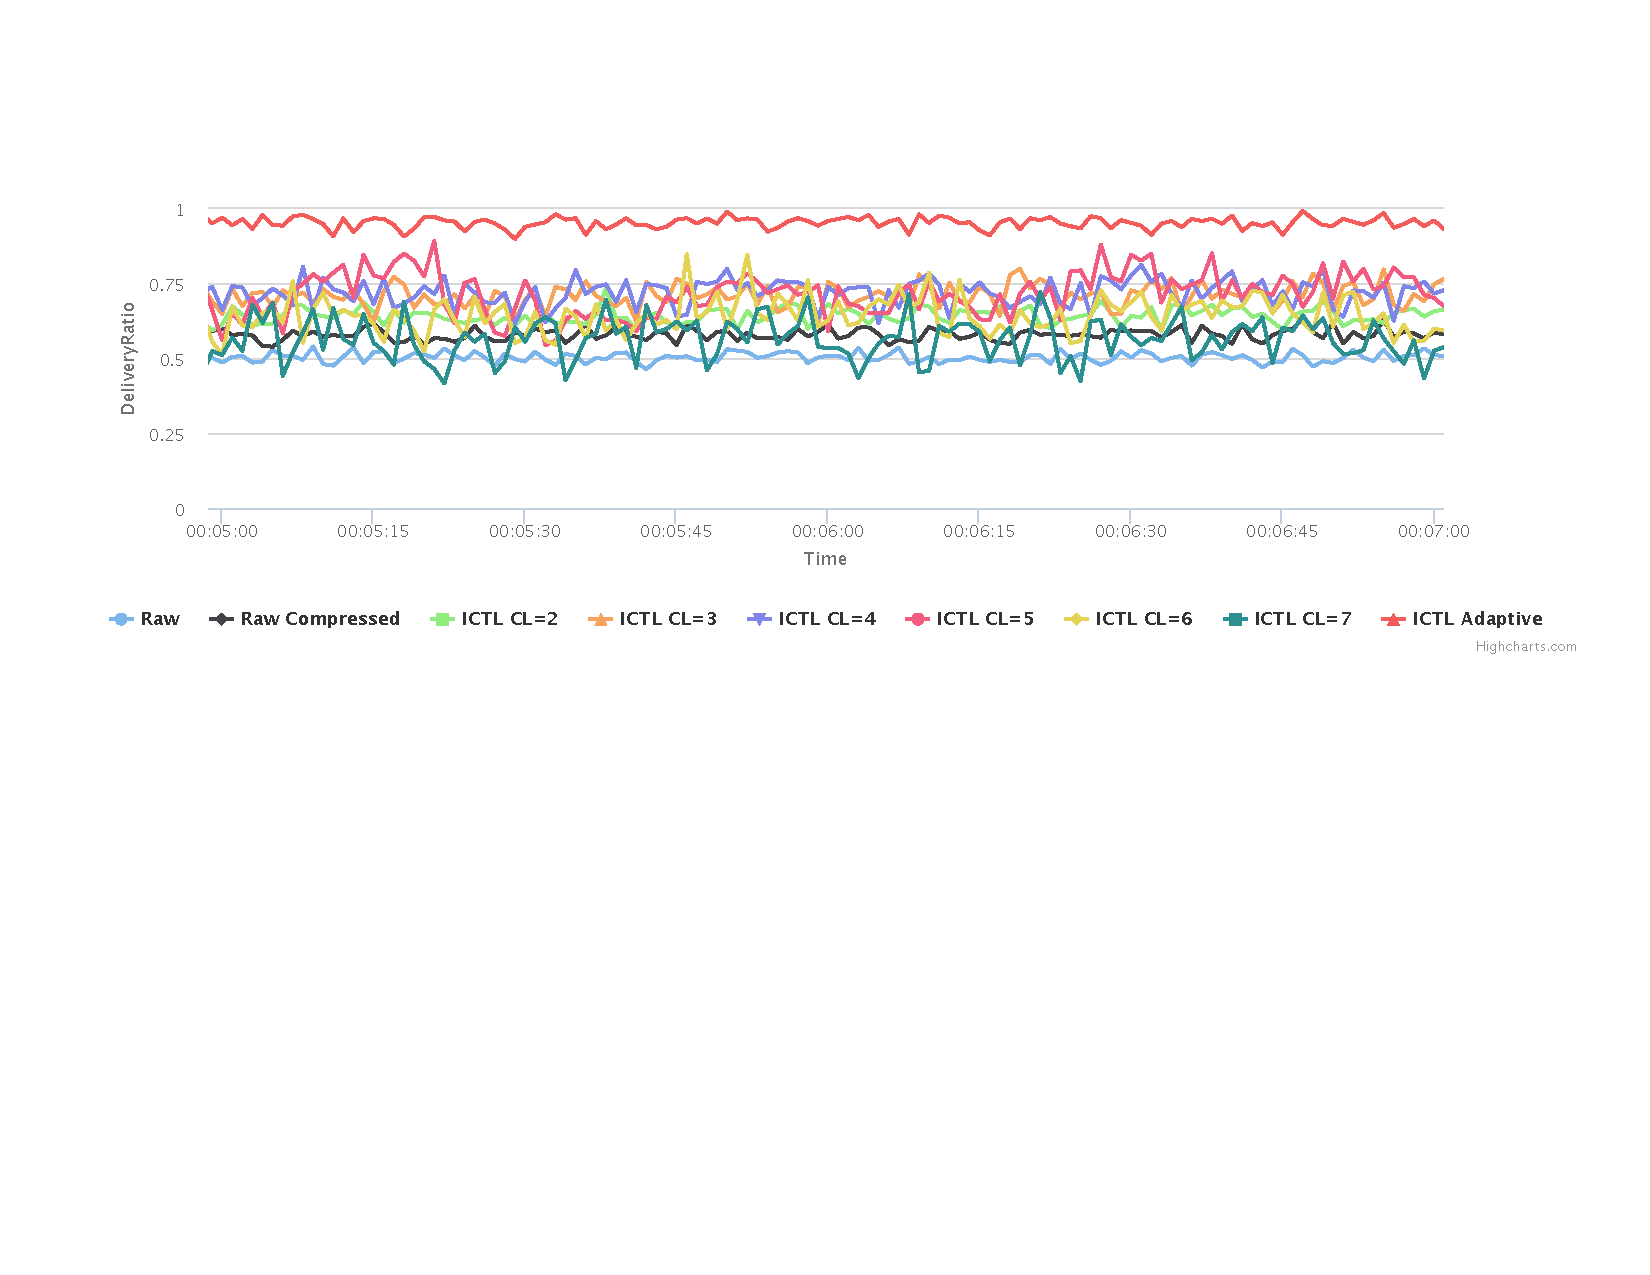
\includegraphics[width=1.1\textwidth]{figures/results/adaptive_adr-10_zoom.pdf}}
  \caption{\label{fig:adaptive_adr_10}ADR in adaptive ICTL compared other transmission strategies with 10 nodes: 30-minute view and 2-minute zoom-in view}
\end{figure}

Figure~\ref{fig:adaptive_adr_10} shows ADR results when there are 10 nodes in emulation. In this case, congestion starts to happen for ICTL with fixed CL settings. However, adaptive ICTL still delivers close to 100\% of messages.

\begin{figure}[H]
  \makebox[\textwidth][c]{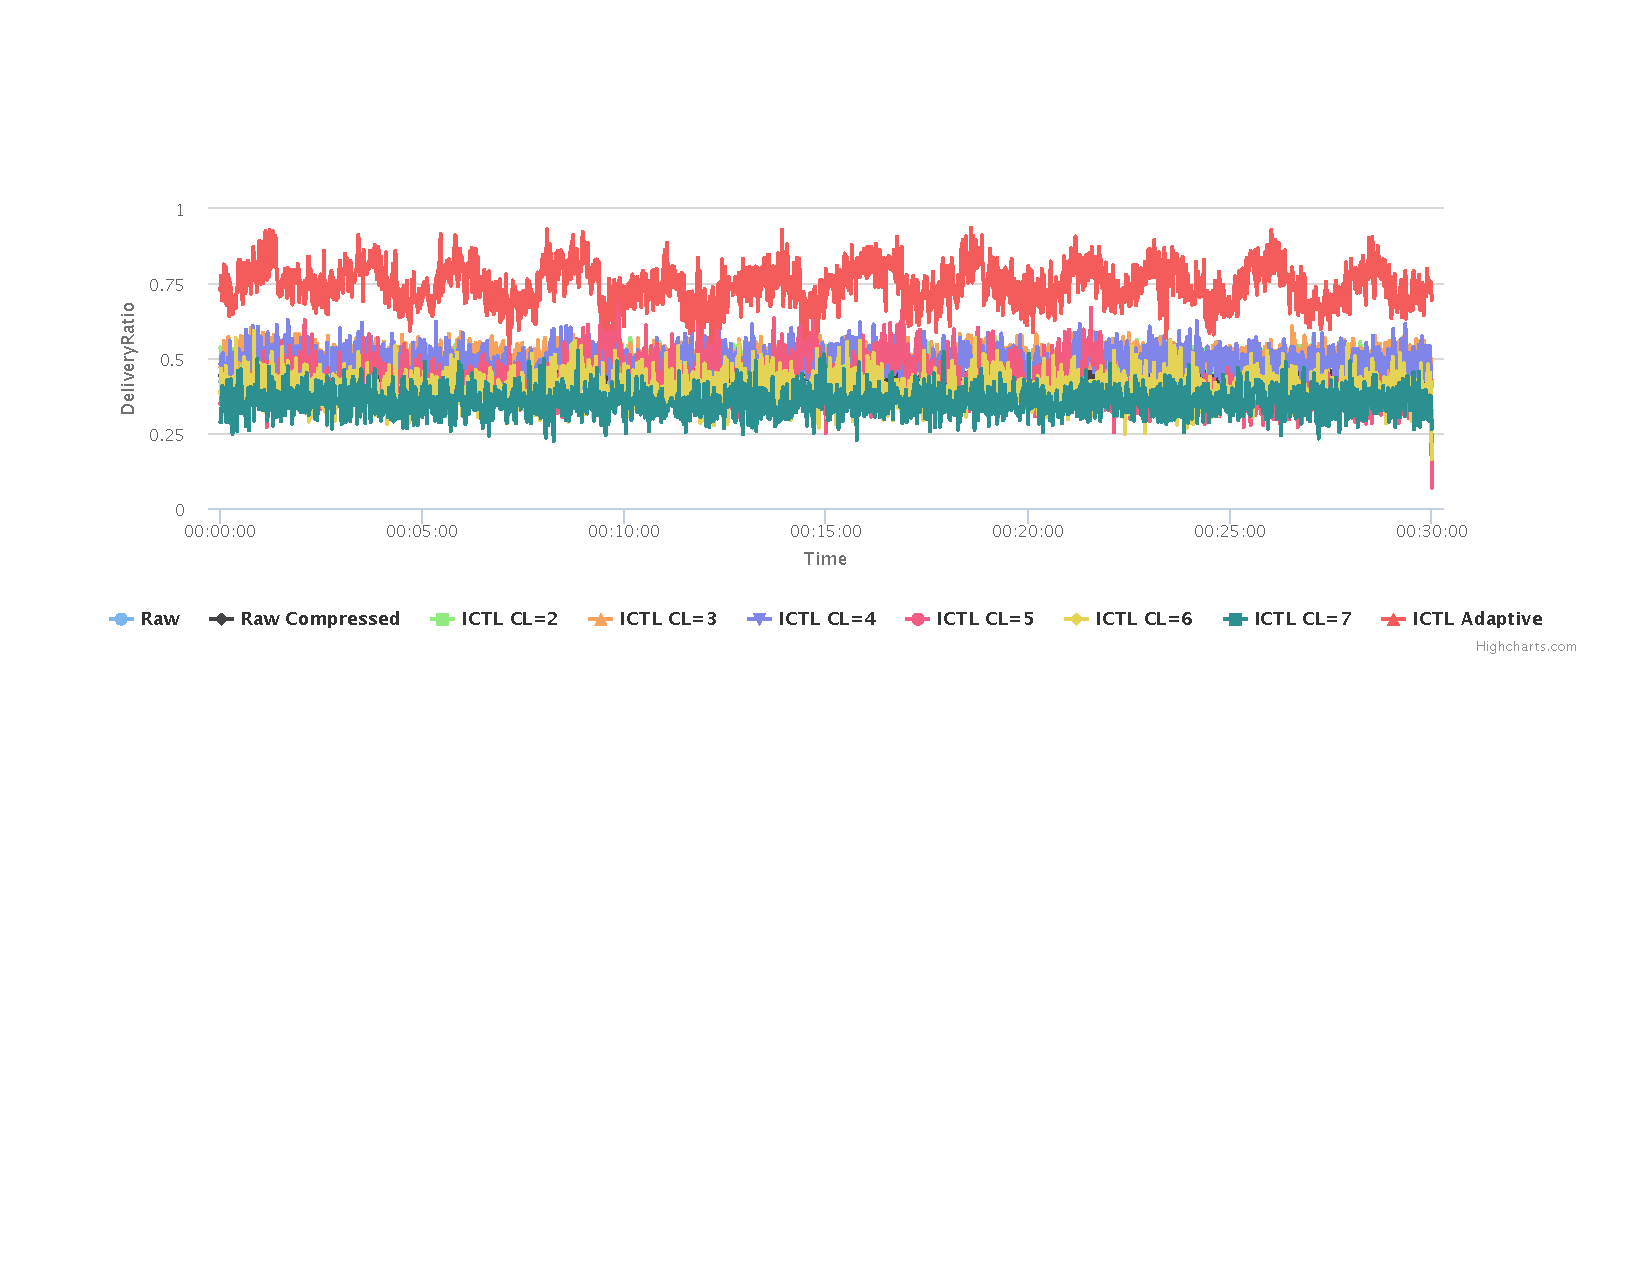
\includegraphics[width=1.1\textwidth]{figures/results/adaptive_adr-12.pdf}}
  \makebox[\textwidth][c]{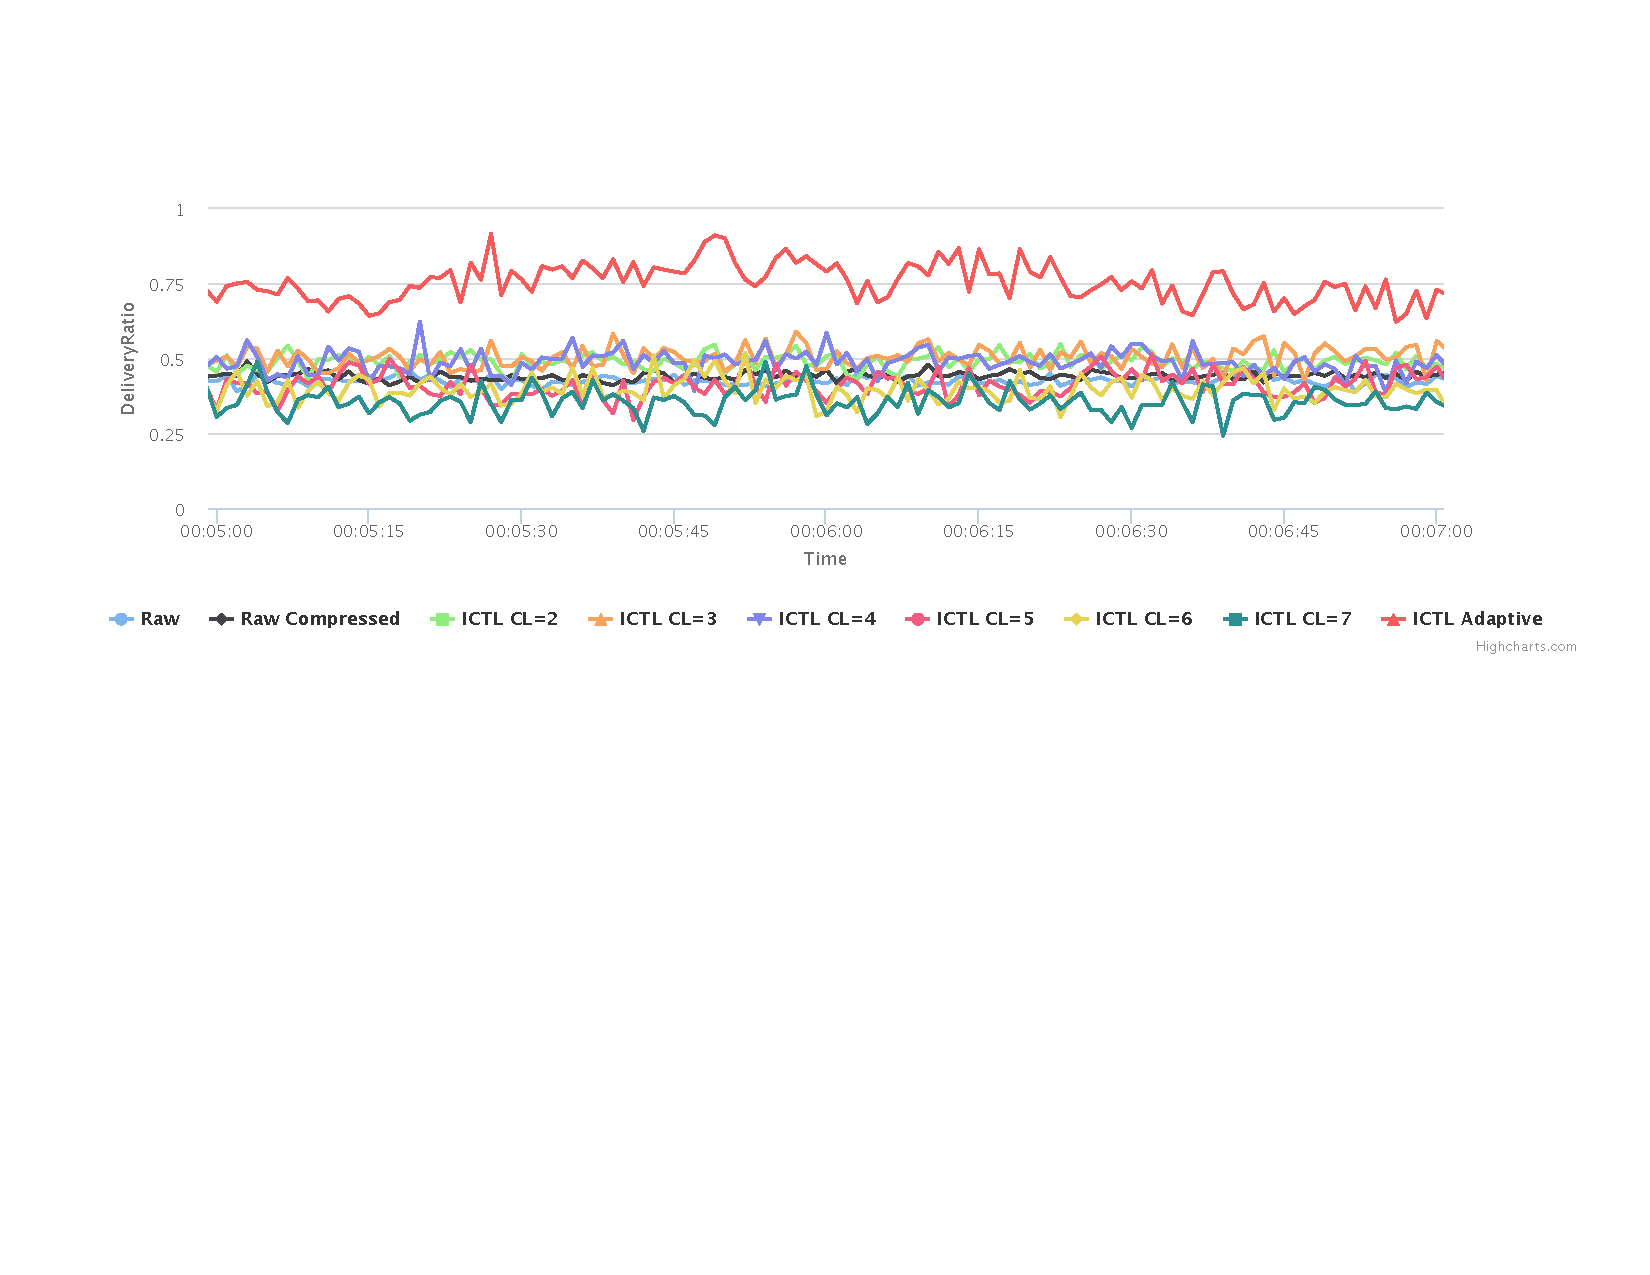
\includegraphics[width=1.1\textwidth]{figures/results/adaptive_adr-12_zoom.pdf}}
  \caption{\label{fig:adaptive_adr_12}ADR in adaptive ICTL compared other transmission strategies with 12 nodes: 30-minute view and 2-minute zoom-in view}
\end{figure}

Figure~\ref{fig:adaptive_adr_12} shows ADR results when there are 12 nodes in emulation. In this case, even adaptive ICTL starts to suffer from congestion. Although, even with congestion, adaptive ICTL still has the best ADR among all transmission strategies.

Putting these results together, Figure~\ref{fig:adaptive_adr_aggr} aggregates results from emulations with different number of nodes into a single plot, showing ADR in different transmission strategies, with different number of nodes in emulation.

\begin{figure}[H]
  \makebox[\textwidth][c]{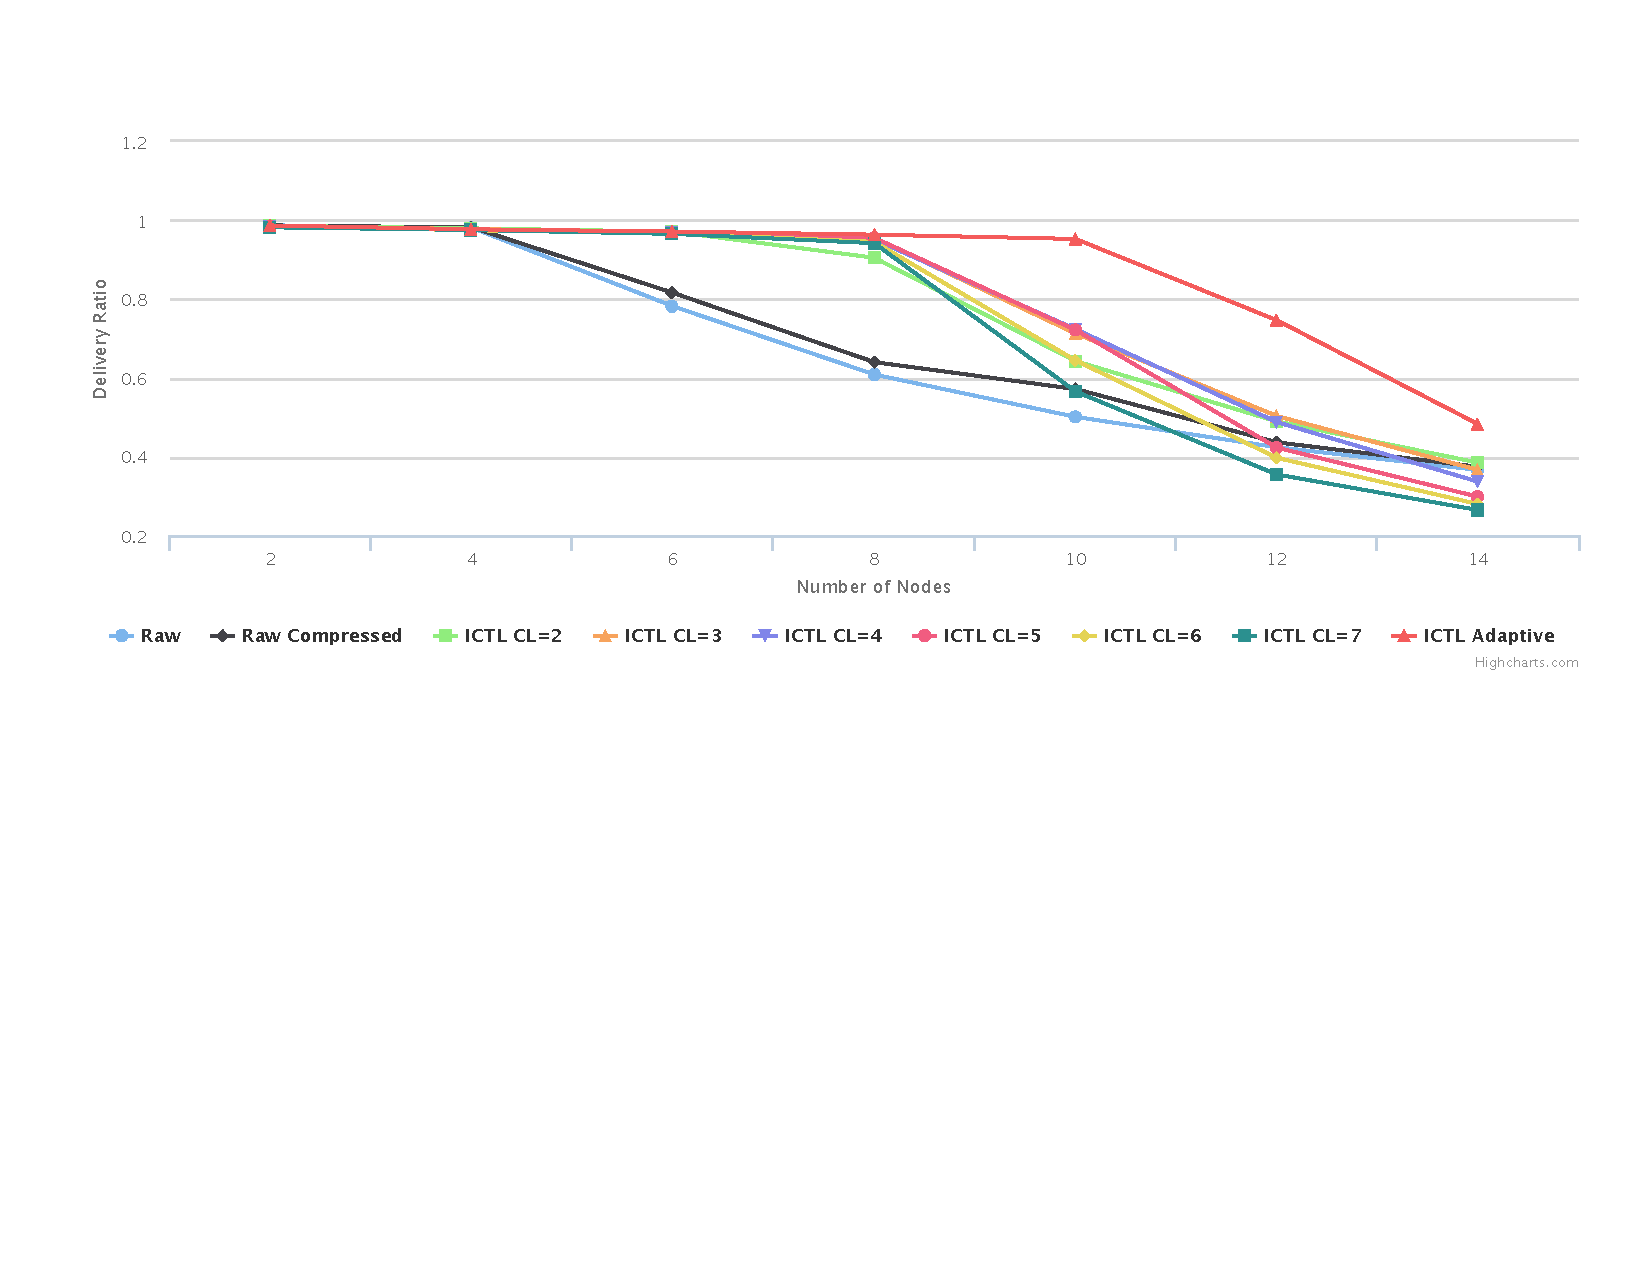
\includegraphics[width=1.1\textwidth]{figures/results/adaptive_adr.pdf}}
  \caption{\label{fig:adaptive_adr_aggr}ADR in adaptive ICTL compared other transmission strategies with different node configurations aggregated in one plot}
\end{figure}

As shown in figures, adaptive ICTL has the best ADR among all fixed CL settings, and has significantly high ADR compared to original data trace or using a traditional compression algorithm, when wireless channel is congested.

In addition, Adaptive ICTL also postpone the point when congestion happens, thus pushes back the point when a congestion control algorithm needs to be activated. This helps maintain a high service level of DSRC networking services.

\section{ICTL Running Time Benchmarks}

Adaptive ICTL is a fairly complicated process compared to simple networking operations such as sending a packet. To study the processing efficiency of adaptive ICTL, some benchmarks are done against adaptive ICTL to study running time of the encoding process, using Go's built-in benchmark framework, on a laptop computer with Intel(R) Core(TM) i5-5287U processor.

In the benchmarks, adaptive ICTL is configured to either automatically select compression algorithm by iterating through 4 algorithms, or always use \texttt{flate}. The data trace is composed of messages that are either completely random, or always identical to each other. With random data, differential data is large, thus it takes more time for adaptive ICTL to compress the payload. With identical data, differential data is full of zeros, and it takes significantly less time for adaptive ICTL to compress the payload. Thus, identical data determines the lower bound of running time of adaptive ICTL, while random data trace is a good estimate of upper bound.

\begin{table}[h]
  \begin{center}
    \begin{tabular}{|c|r|r|}
      \hline
      Unit: ns/op & Random & Identical \\ \hline
      Iterating   & 2,434,206 & 1,232,683 \\ \hline
      Flate       & 701,801 & 305,154 \\ \hline
    \end{tabular}
    \caption{\label{tab:ictl_time_256}Adaptive ICTL Running Time Benchmarks: 256-byte messages}
  \end{center}
\end{table}

\begin{table}[h]
  \begin{center}
    \begin{tabular}{|c|r|r|}
      \hline
      Unit: ns/op & Random & Identical \\ \hline
      Iterating   & 2,942,048 & 1,318,164 \\ \hline
      Flate       & 882,314 & 321,307 \\ \hline
    \end{tabular}
    \caption{\label{tab:ictl_time_1024}Adaptive ICTL Running Time Benchmarks: 1024-byte messages}
  \end{center}
\end{table}

Table~\ref{tab:ictl_time_256} shows running time of encoding operations of 4 configurations, for data traces composed of 256-byte messages. With fixed \texttt{flate} compression, the running time per operation is about 0.3 ms for identical data, and around 0.7 ms for random data.

Table~\ref{tab:ictl_time_1024} shows results for 1024-byte messages. Identical data and random data takes about 0.3 ms and 0.8 ms to encode respectively. With larger message size, running time of each operation is slightly larger, but not significantly larger. This suggests that larger message size does not affect adaptive ICTL encoding time significantly.

This suggests that, users of adaptive ICTL should be prepared that adaptive ICTL can cause up to 1 ms delay. 1 ms is comparable to the time it takes for networking stack on a device to send a network packet. Depending how critical 1 ms is to the application, and how efficient the rest of networking stack is, this can be significant. Implementing other operations asynchronously can help improve overall system response time, whereas the running time of ICTL is a hard limit. Thus, whether or not to use ICTL is a matter of trade-offs between low latency and low bandwidth consumption.

\section{Conclusion}

This chapter introduces an ICTL algorithm as a way to reduce bandwidth consumption in DSRC applications. The ICTL algorithm is implemented and tested on Squirrel. Behaviors of ICTL under different scenarios and configurations have been studied. Guided by the findings, an even lower bandwidth consuming algorithm, adaptive ICTL, is designed.

By using adaptive ICTL, bandwidth consumption of the platooning data trace used in this study is reduced by over 50\% in size. Consequently, in congested networking environment, adaptive ICTL delivers the highest ADR in all tested transmitted strategies. Thus, Adaptive ICTL helps postpone the point when congestion control algorithms have to be activated, which indirectly improves the service reliability of DSRC networking in vehicular environments.

The running time of adaptive ICTL's encoding operation is less than 1 ms, but greater than 0.3 ms. Depending on how sensitive the application is to latencies, this may or may not be significant.

\chapter{Summary}

In context of a real-world application, vehicle platooning, this dissertation strives to improve efficiency and reliability of vehicular networking, using an emulated experimental approach.

To start with, an emulation infrastructure is designed and implemented to provide a scalable yet realistic experimental platform. As a general framework for wireless networking emulation, Squirrel is designed to use as much real-world software components as possible. Conceptually, it replaces the wireless hardware, device driver's Hardware Abstract Layer (HAL) and the IEEE 802.11 kernel module, and provides upper layers with interfaces that are same as on real wireless devices. Consequently, testing targets on Squirrel are real software components that are deployable to real-world devices. Squirrel is configurable through a plug-in system. This allows different wireless models and mobility managers to be developed for Squirrel.

Studies in this dissertation use a CSMA/CA model that emulates the behaviors of IEEE 802.11 networks. It uses a leaky bucket to track channel condition in vicinity of each node. As an event happens near a node, the corresponding leaky bucket increases by the number of nanoseconds the event takes to finish. All leaky buckets leak at the same rate as time, i.e. $1\times 10^9$ per second. With this technique, channel condition is independently tracked for each node, which enables the model to not only shape throughput of traffic, but also reflect interference generated by other transmitting nodes. As a result, channel congestion is properly emulated.

Effectiveness tests are conducted for the CSMA/CA model in Squirrel. It demonstrates that Squirrel effectively reflect network congestion in the test, and show a similar trend of iperf UDP throughput compared to the same test conducted on Android devices. In addition, Squirrel's throughput is also tested using the PassThrough network model. On a workstation with a 6-core CPU, Squirrel achieves 1200 Mbps throughput in total.

Second, an interframe compression method, ICTL, is designed and implemented. Unlike traditional compression methods where payload of each frame is compressed directly, ICTL compresses the difference between consecutive frames. The interframe compression design is inspired by video compression algorithms, but is adapted to be more suitable for vehicular networking. Two message types, KF and DF, are introduced by ICTL. A KF encodes application data directly, while DF encodes the difference between the application data and a previously transmitted KF. In a general transmission sequence, a KF is followed by a number of DFs. Since a DF is much smaller than a KF, this reduces average bandwidth consumption.

Behaviors of ICTL are studied under different configurations and scenarios, using analytical method as well as experimental method on Squirrel. Based on mathematical analysis, it is speculated that reducing bandwidth consumption should help increase ADR as well. With this in mind, an adaptive ICTL is designed and implemented. Unlike in basic ICTL where a fixed CL is used, adaptive ICTL goes through a process for each frame to determine whether it should be a KF or a DF should be send, based on average frame size within current ICTL Cycle.

The adaptive ICTL was tested on Squirrel, under different network utilization level. It has been shown that adaptive ICTL achieves over 50\% in reduction of bandwidth consumption, and maintains relative high ADR when network is congested. The adaptive ICTL algorithm achieves the lowest bandwidth consumption and highest ADR among all tested ICTL and tradition compression algorithms, in all test cases.

\chapter{Future Work}

As an extension of this work, multi-hop scenarios can be studied. This chapter describe a general idea of using Multi-Point Relays (MPRs\nomenclature{MPR}{Multi-Point Relay}) in multi-hop vehicular networks.

In this study, the effort has been focused on improving efficiency and reliability in single hop transmissions. However, for large vehicle platoons, this is not sufficient. Normally one of vehicles in the platoon serves as controller, and helps with coordinating different vehicles. As a result, it is important that platooning messages from the control vehicle can reach all vehicles in the platoon. For large platoons that are composed of many vehicles, it is normally impossible to transmit message from one end of platoon all the way to the other end within one hop. Hence, an efficient yet reliable rebroadcasting scheme needs to be developed for platooning applications.

One of the ways to design such a rebroadcasting scheme is to use MPRs. MPR is a concept proposed by Optimized Link State Routing (OLSR\nomenclature{OLSR}{Optimized Link State Routing}) Protocol \cite{rfc3626}. As its name suggests, a MPR node relays messages for other nodes. To be more specific, each node has a minimum set of 1-hop neighbors as MPRs, so that there exists a path to each of its 2-hop neighbors via a node selected as an MPR. This way, a naive broadcast reaches all 1-hop neighbors, while MPRs relays the messages to 2-hop neighbors. Since only a subset of 1-hop neighbors are selected as MPRs, this reduces relaying overhead significantly. OLSR uses MPRs to relay routing information, but the concept of MPRs can be used for general purpose flooding as well. In vehicular network, platooning applications can construct MPRs to propagate platooning messages within the entire platoon.

To calculate MPR set, each node needs to know its 1-hop neighbors and 2-hop neighbors. OLSR uses Hello message and Topology Control (TC\nomenclature{TC}{Topology Control}) messages to discover local topology. A hello message is like a beacon, which contains the node's basic information and allows nodes to discover 1-hop neighbors. A TC message contains all 1-hop neighbors of the node, which allows its 1-hop neighbors to sense 2-hop neighbors. These two messages are broadcast periodically by each node.

For a dynamic network like vehicular network, it is important to keep MPR set up to date in order to achieve good delivery ratio. The frequency that these messages are broadcast is a key parameter to performance. If the messages are broadcast too frequently, they generate a lot of overhead. If the messages are too infrequent, the MPR set may often be out of date, especially for a dynamic network where topology changes very often.

In vehicular networks, vehicles are already broadcasting beacon-like messages through WSMP, such as BSM. These messages allows all vehicles sense 1-hop neighbors. If the vehicles construct TC messages as well, they can select MPRs in the same way as OLSR. This is a viable and straight-forward solution, but may cause large overhead for vehicular network, since the topology is more dynamic due to traffic condition, road condition, and terrains nearby.

Fortunately, applications running on vehicles have access to vehicular dynamics data as well as GPS positions. They enable some interesting ways to maintain a healthy MPR set for each node.

\begin{itemize}
  \item GPS information can be used to assist selecting MPRs. The 1-hop neighbor set constructed with beacon messages provide information on communication range. Assuming that this range does not change dramatically within short period of time, it can be used to estimate 2-hop neighbors, allowing selecting MPR set without TC messages.
  \item Vehicular dynamics data provides a history as well as current status of the vehicle's speed, acceleration, and steering information. Along with GPS positions, it is possible to predict each vehicle's trajectory. This is particularly useful when a vehicle is about to leave the platoon, or when a new vehicle is joining the platoon. This is the time when network topology of the platoon changes dramatically. Prediction on such an event allows each vehicle in the platoon to adjust MPR set accordingly to avoid high message loss rate by temporarily rebroadcasting more aggressively.
\end{itemize}

In short, vehicular environment and DSRC provide a way to construct MPR set without introducing TC messages to the system, and a way for vehicles to predict topology changes, making them more responsive to dynamic environments.

A properly designed MPR algorithm for DSRC applications can reduce bandwidth consumption, thus improving ADR for multi-hop transmissions. Thus, this is a promising direction to improve vehicular networking efficiency and reliability for DSRC applications.


\bibliographystyle{IEEEtran}
\bibliography{bib}

\chapter*{Postface}
\addcontentsline{toc}{chapter}{Postface}%

Research projects ultimately serve humanity. In exploring the unknowns, seeking challenges, and enjoying the joy of solving problems, we should always strive to discover possibilities to make the world a better place to live in.

The author truly believes that research should be driven by real-world problems, and that, research should be reproducible and applicable in real-world. This belief has led to the efforts towards the real-world data driven, realistic targeted emulation approach used in this dissertation.

\vspace{4em}

\begin{figure}[h]
  \begin{center}
  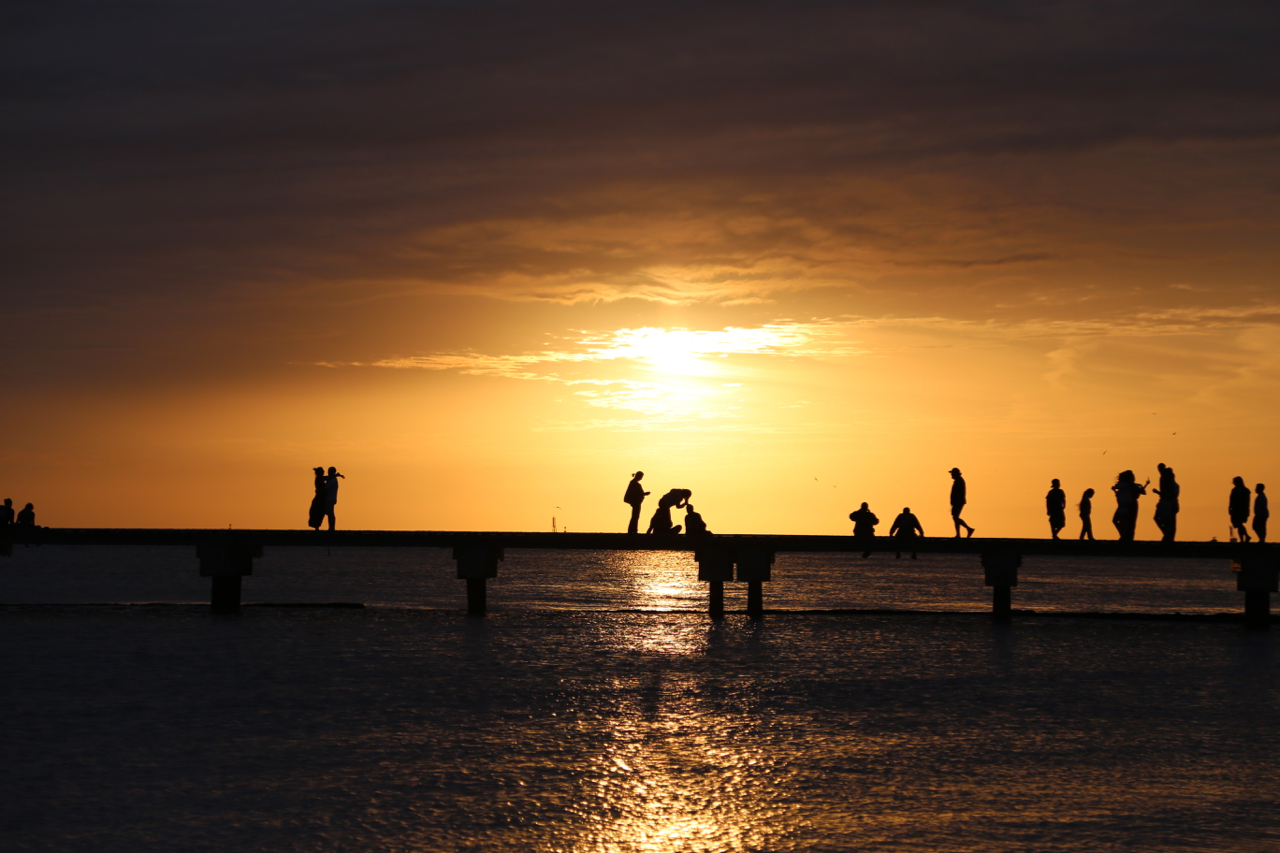
\includegraphics[width=.8\textwidth]{figures/postface.jpg}
  \end{center}
\end{figure}



\end{document}

